\chapter{Geometrie auf der Kugeloberfläche\label{chapter:kugel}}
\lhead{Geometrie auf der Kugeloberfläche}
\begin{refsection}
\chapterauthor{Melina Staub und Fabian Schmid}

\section{Einleitung}
Seit jeher fasziniert den Menschen die Fahrt zur See. Nicht grundlos ist die Seefahrt eine der wichtigsten und ältesten Tätigkeiten der Menschheit. Der innere Drang neue Weltmeere und unbekannte Gebiete zu entdecken, die Fahrt zur See zu erleichtern und erträglicher zu machen, trieben die Menschen an, die Schiffe dieser Welt immer weiter zu entwickeln.
In der Seefahrt spielte auch die Form der Erde eine wichtige Rolle. Den die Idee der Erde als Kugel ist älter als man zu denken vermag. Bereits der Schüler des antiken griechischen Philosophen Platon - Aristoteles beschrieb in seiner Schrift \textit{Über den Himmel} aus dem 4. Jahrhundert v. Chr. etliche Gründe welche für die Gestalt der Erde als Kugel sprechen:
\begin{itemize}
      \item Sämtliche schweren Körper streben zum Mittelpunkt des Alls. Da sie dies von allen Seiten her gleichmässig tun und die Erde im Mittelpunkt des Alls steht, muss sie eine kugelrunde Gestalt annehmen. 
\item Bei von der Küste wegfahrende Schiffen wird der Rumpf vor den Segeln der Sicht verborgen. 
\item In südlichen Ländern erscheinen südliche Sternbilder höher über dem Horizont.
\item Der Erdschatten bei einer Mondfinsternis ist stets rund.
\end{itemize}

Jedoch war um 1492 der Zeit der Entdeckung Amerikas durch Christoph Kolumbus, die Idee der Erde in Kugelform noch sehr umstritten. Er erkannte anhand Theorien und Erkenntnissen der alten Griechen, jenen von Aristoteles, das die Erde eine Kugel sein muss.

Mit seinem Vorschlag einen Seeweg über den Atlantik nach Indien zu finden und nicht wie üblich um Afrika zu segeln, stiess er beim portugiesischen König auf taube Ohren. Sein Plan Indien über eine Route nach Westen zu erreichen, widersprach dem gesunden Menschenverstand. Wäre die Erde wirklich eine Kugel und man befände sich auf der unteren Erdhalbkugel, würde man dann nicht herunterfallen? Jedoch brachte auch der damalige Glaube an die Erde in Scheibenform so einige Risiken mit sich. Was würde passieren, wenn die Flotte den Rand der Scheibe erreicht hatte? Würden sie über den Erdrand hinweggleiten und in den Abgrund stürzen?

Erst nach viel Überzeugungsarbeit durch Kolumbus, setzte er sich am spanischen Hof durch und segelte über die westliche Route über den Atlantik und entdeckte schlussendlich Amerika - nicht Indien.
Der praktische und greifbare Beweis, dass die Erde eine Kugel ist, lieferte rund 30 Jahre später der Portugiese Fernando Magellan. Mit seiner Weltumsegelung und der Ankunft in den Philippinen, bewies er definitiv das die Erde eine Kugelgestalt hat.

Nun wollen wir uns die Frage stellen, wie die alten Seefahrer ohne GPS und jeglichen modernen Navigationssystemen auf hoher See, wussten wo sie sich befanden und was die Sterne mit alledem zu tun haben. Reisen Sie mit uns zurück in eine Zeit der Sextanten, Kompasse und Sternkarten - In die Zeit der Seefahrer und Entdecker.



\section{Gross- und Kleinkreise}
Eine Kugeloberfläche lässt sich in zwei verschiedene Kreisarten einteilen: Gross- und Kleinkreise. 
Wir betrachten als erstes die Grosskreise:

\subsection{Grosskreise}
Es gibt unendlich viele Möglichkeiten eine Kugel in zwei gleich grosse Stücke zu zerschneiden, daher gibt es auch unendlich viele Grosskreise.

\begin{definition}
\textit{Ein Grosskreis ist ein grösstmöglicher Kreis auf einer Kugeloberfläche. Sein Mittelpunkt fällt immer mit dem Mittelpunkt der Kugel zusammen und ein Schnitt auf dem Grosskreis teilt die Kugel (auf jedem Fall) in zwei (gleich grosse) Hälften.}
\label{skript:kugel:satz:Grosskreis}
\index{Grosskreis}
\end{definition}

\begin{center}
        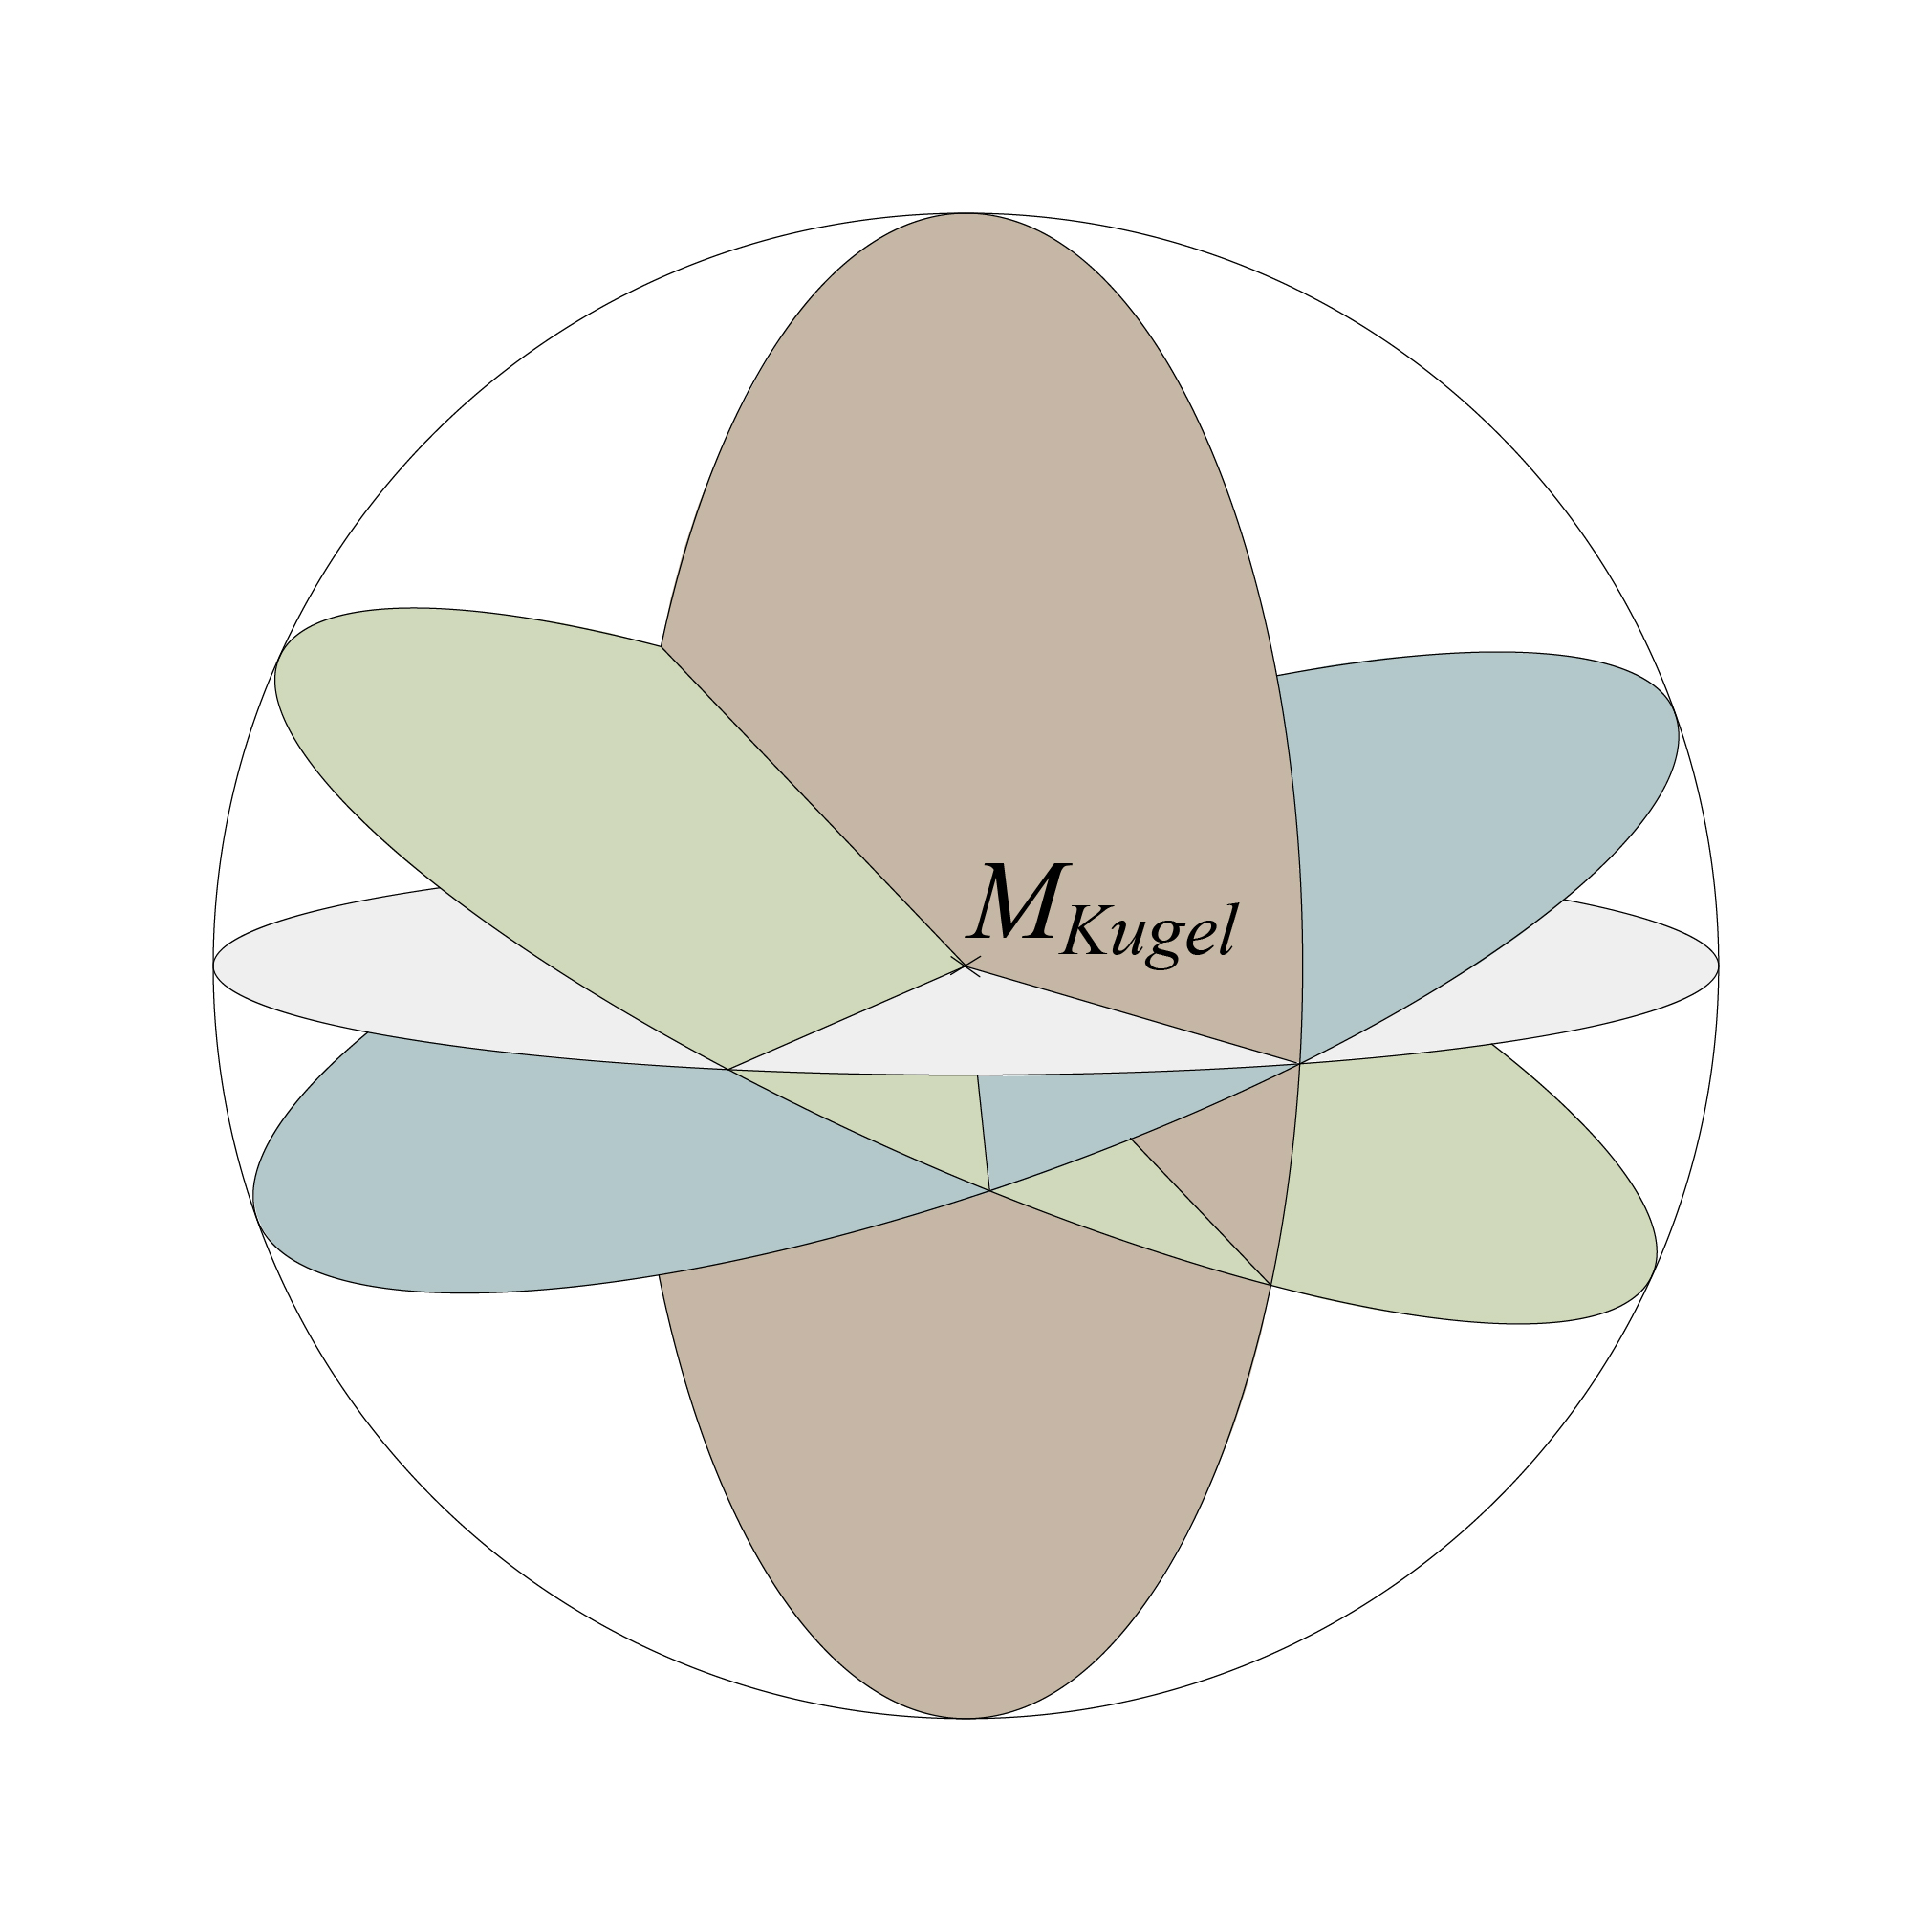
\includegraphics[width=0.4\textwidth]{kugel/Grosskreise.jpg}
    \captionof{figure}{Verschiedene Grosskreise auf einer Kugel}
\end{center}

Mithilfe der Schnittpunkte verschiedener Grosskreise, lassen sich sphärische Dreiecke bilden, auf welchen sich die sphärische Trigonometrie anwenden lässt.

Um unseren Standort auf der Erde klar zu bestimmen, wurde diese in ein Raster von Grosskreisen unterteilt. Diese stehen orthogonal zum Äquator und sind uns bekannt als Längengrade.


\subsection{Kleinkreise}
Die Kleinkreise eignen sich im Gegensatz zu den Grosskreisen \textit{nicht} für die sphärische Trigonometrie.  Dies liegt daran, dass sie keinen einheitlichen Mittelpunkt haben und so nicht zwingend den Radius haben.
Sie werden lediglich zur Bestimmung von Messgrössen, Winkelabstände oder des Höhenwinkels eines Gestirns verwendet. 

\begin{definition}
Unter Kleinkreis versteht man jene Kreise auf einer Kugeloberfläche, deren Ebenen nicht den Kugelmittelpunkt enthalten. Davon ausgenommen ist der Äquator, er bildet einen Gross- und Kleinkreis gleichermassen.
\label{skript:kugel:satz:Kleinkreis}
\index{Kleinkreis}
\end{definition} 

\begin{center}
        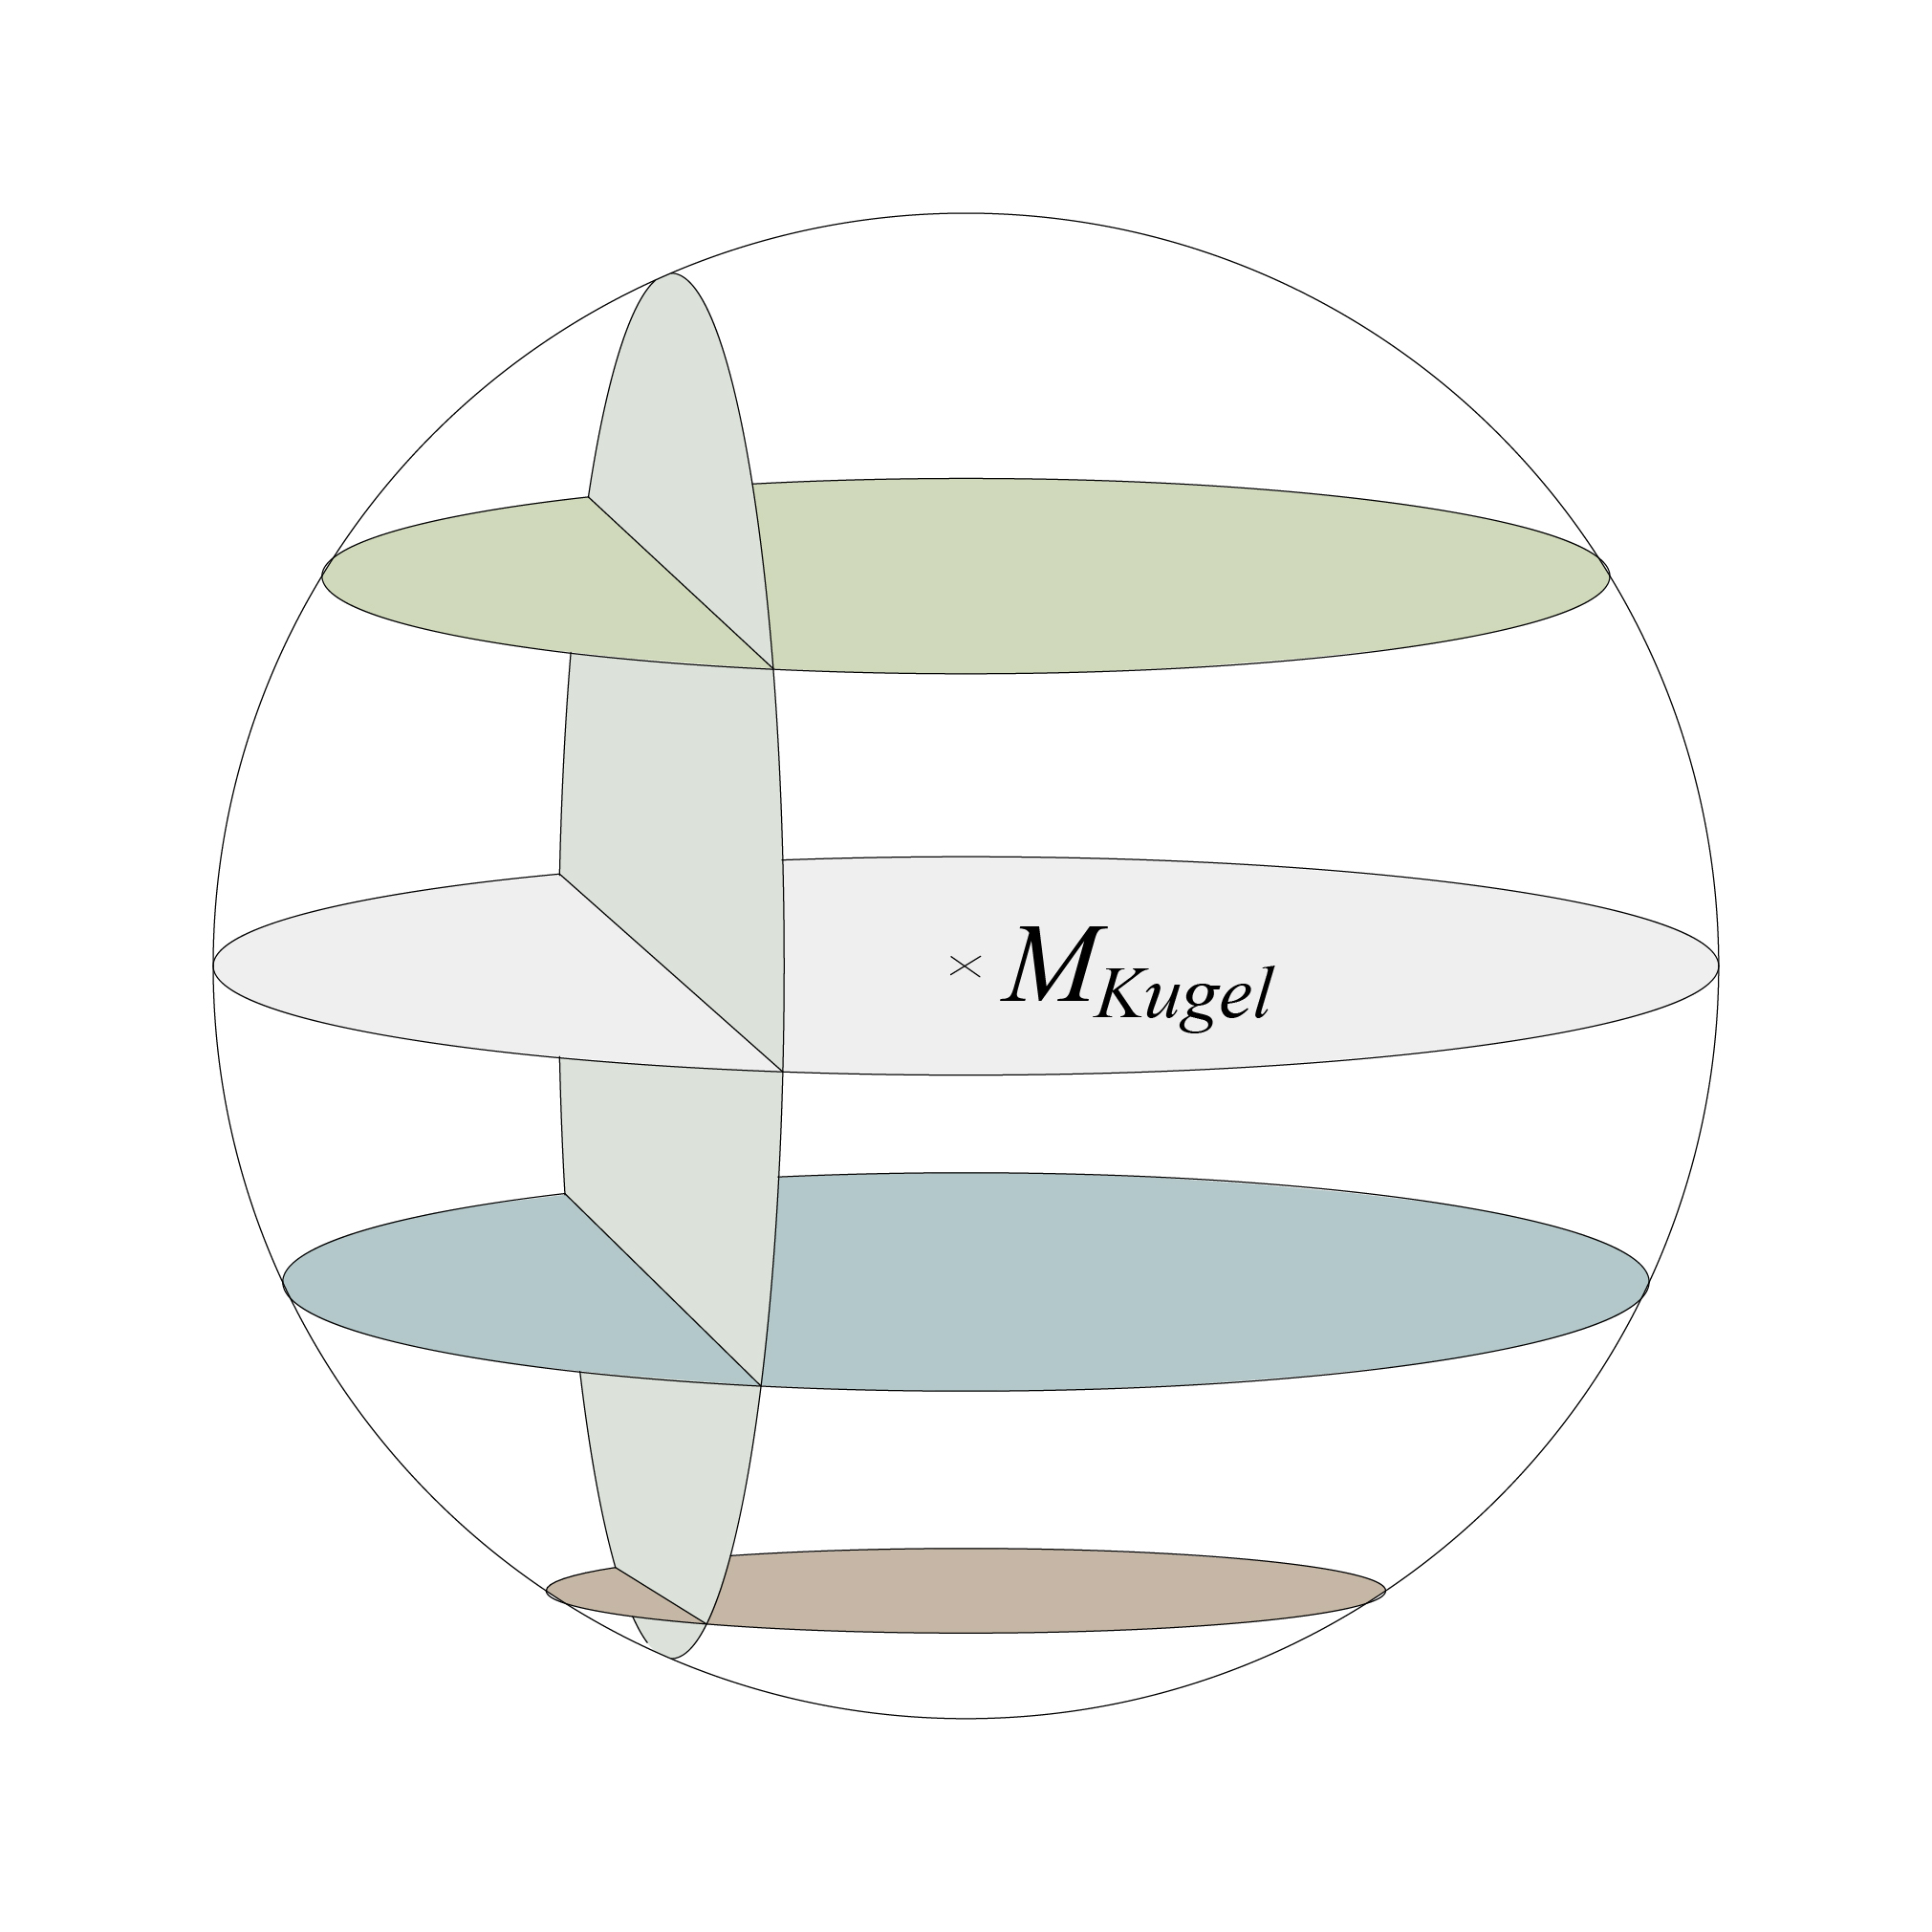
\includegraphics[width=0.4\textwidth]{kugel/Kleinkreise.jpg}
    \captionof{figure}{Verschiedene Kleinkreise auf einer Kugel}
\end{center}

Um unser Raster auf der Erdoberfläche zu vervollständigen und einen eindeutigen Ort auf dem Längengrad zu definieren, benutzen wir die Kleinkreise. Diese verlaufen parallel zum Äquator in Richtung Norden und Süden, wir nennen sie Breitengrade.
Für die Navigation sind sowohl die für die sphärische Trigonometrie hilfreichen Grosskreise (Längengrade) von Nöten wie auch die Kleinkreise (Breitengrade), da man nur mit beiden in Kombination seine Koordinaten eindeutig bestimmen kann.



\section{Sphärische Dreiecke / Kugeldreieck}
Der Begriff sphärisches Dreieck oder Kugeldreieck wird folgendermassen definiert

\begin{definition}
Ein sphärisches Dreieck oder Kugeldreieck, ist eine durch drei Grosskreise begrenzte Figur auf der Kugeloberfläche.
\end{definition} 

Dabei können wir sphärische Dreiecke in drei für uns wesentliche Dreiecksarten unterteilen:

\begin{itemize}
\item Allgemeine Kugeldreiecke (Nicht Eulersche Dreiecke)
\item Kugelzweiecke
\item Eulersche Dreiecke
\item Polardreieck
\end{itemize}


\subsection{Allgemeine Kugeldreiecke (Nicht Eulersche Dreiecke)}
Ähnlich dem Dreieck in der Ebene hat das Dreieck auf der Kugel Seiten und Winkel. Allerdings werden die Dreiecksseiten nicht im Längenmass Meter angegeben, sondern im Bogenmass, denn es handelt sich um Kreisbögen und keine Strecken.
Hinzu kommt, dass die Innenwinkelsumme eines Kugeldreiecks immer grösser als $180^{\circ}$ ist und kann bei allgemeinen Kugeldreiecken bis auf $900^{\circ}$ anwachsen.


\begin{center}
        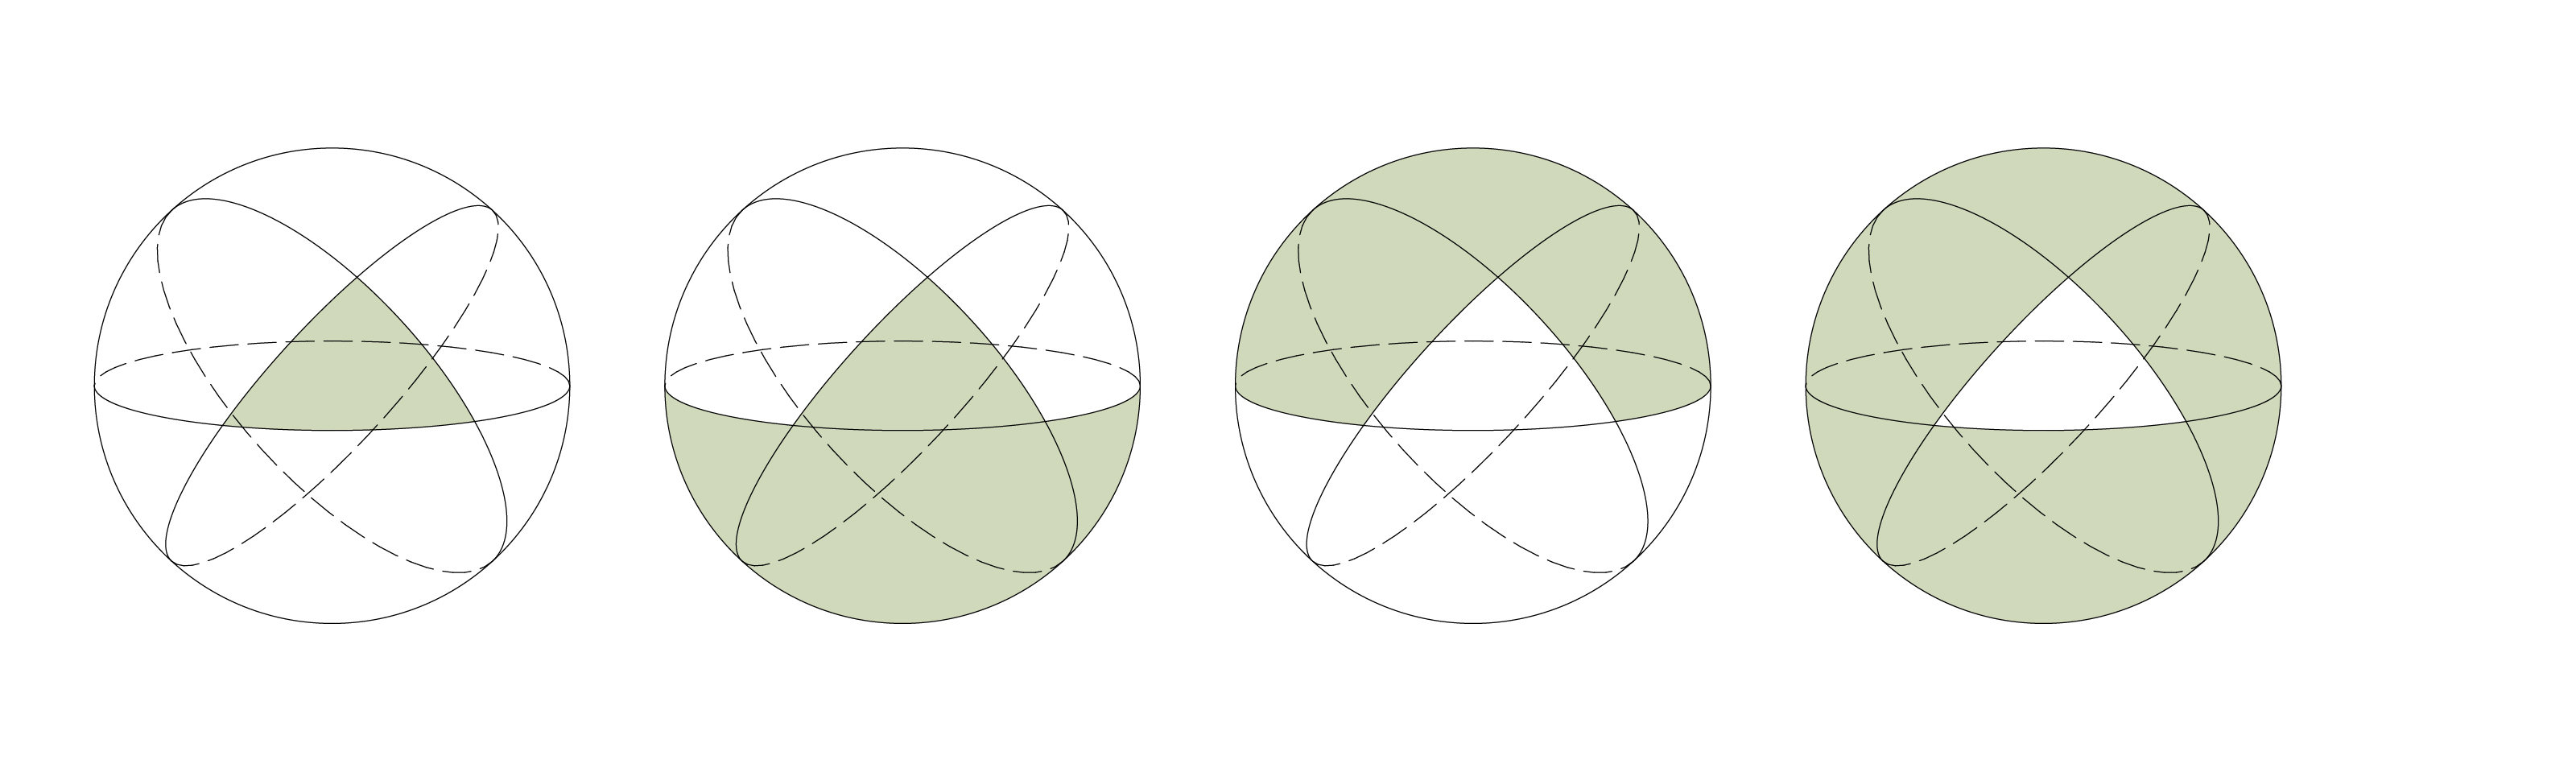
\includegraphics[width=0.9\textwidth]{kugel/Dreiecksarten.jpg}
    \captionof{figure}{Kugeldreiecke auf einer Kugel}
\end{center}


\subsection{Kugelzweiecke} 
Zwei Grosskreise auf der Kugeloberfläche zerlegen diese in paarweise gleich grosse Kugelzweiecke, welche die Kugeloberfläche gleichmässig einnehmen. Würden wir für den Winkel 
$\alpha$ $90^{\circ}$ wählen, würden die Kugelzweiecke je einen Viertel der Kugeloberfläche einnehmen. Die Längen der entstandenen Zweiecksseiten, haben auf jedenfall die Länge
$180^{\circ}$, was auch $\pi$ entspricht.
Der Flächeninhalt wird dabei einzig durch den Winkel $\alpha$ zwischen den beiden Grosskreisen bestimmt, was im Ausdruck \eqref{V5} aufgezeigt wird.

\begin{center}
        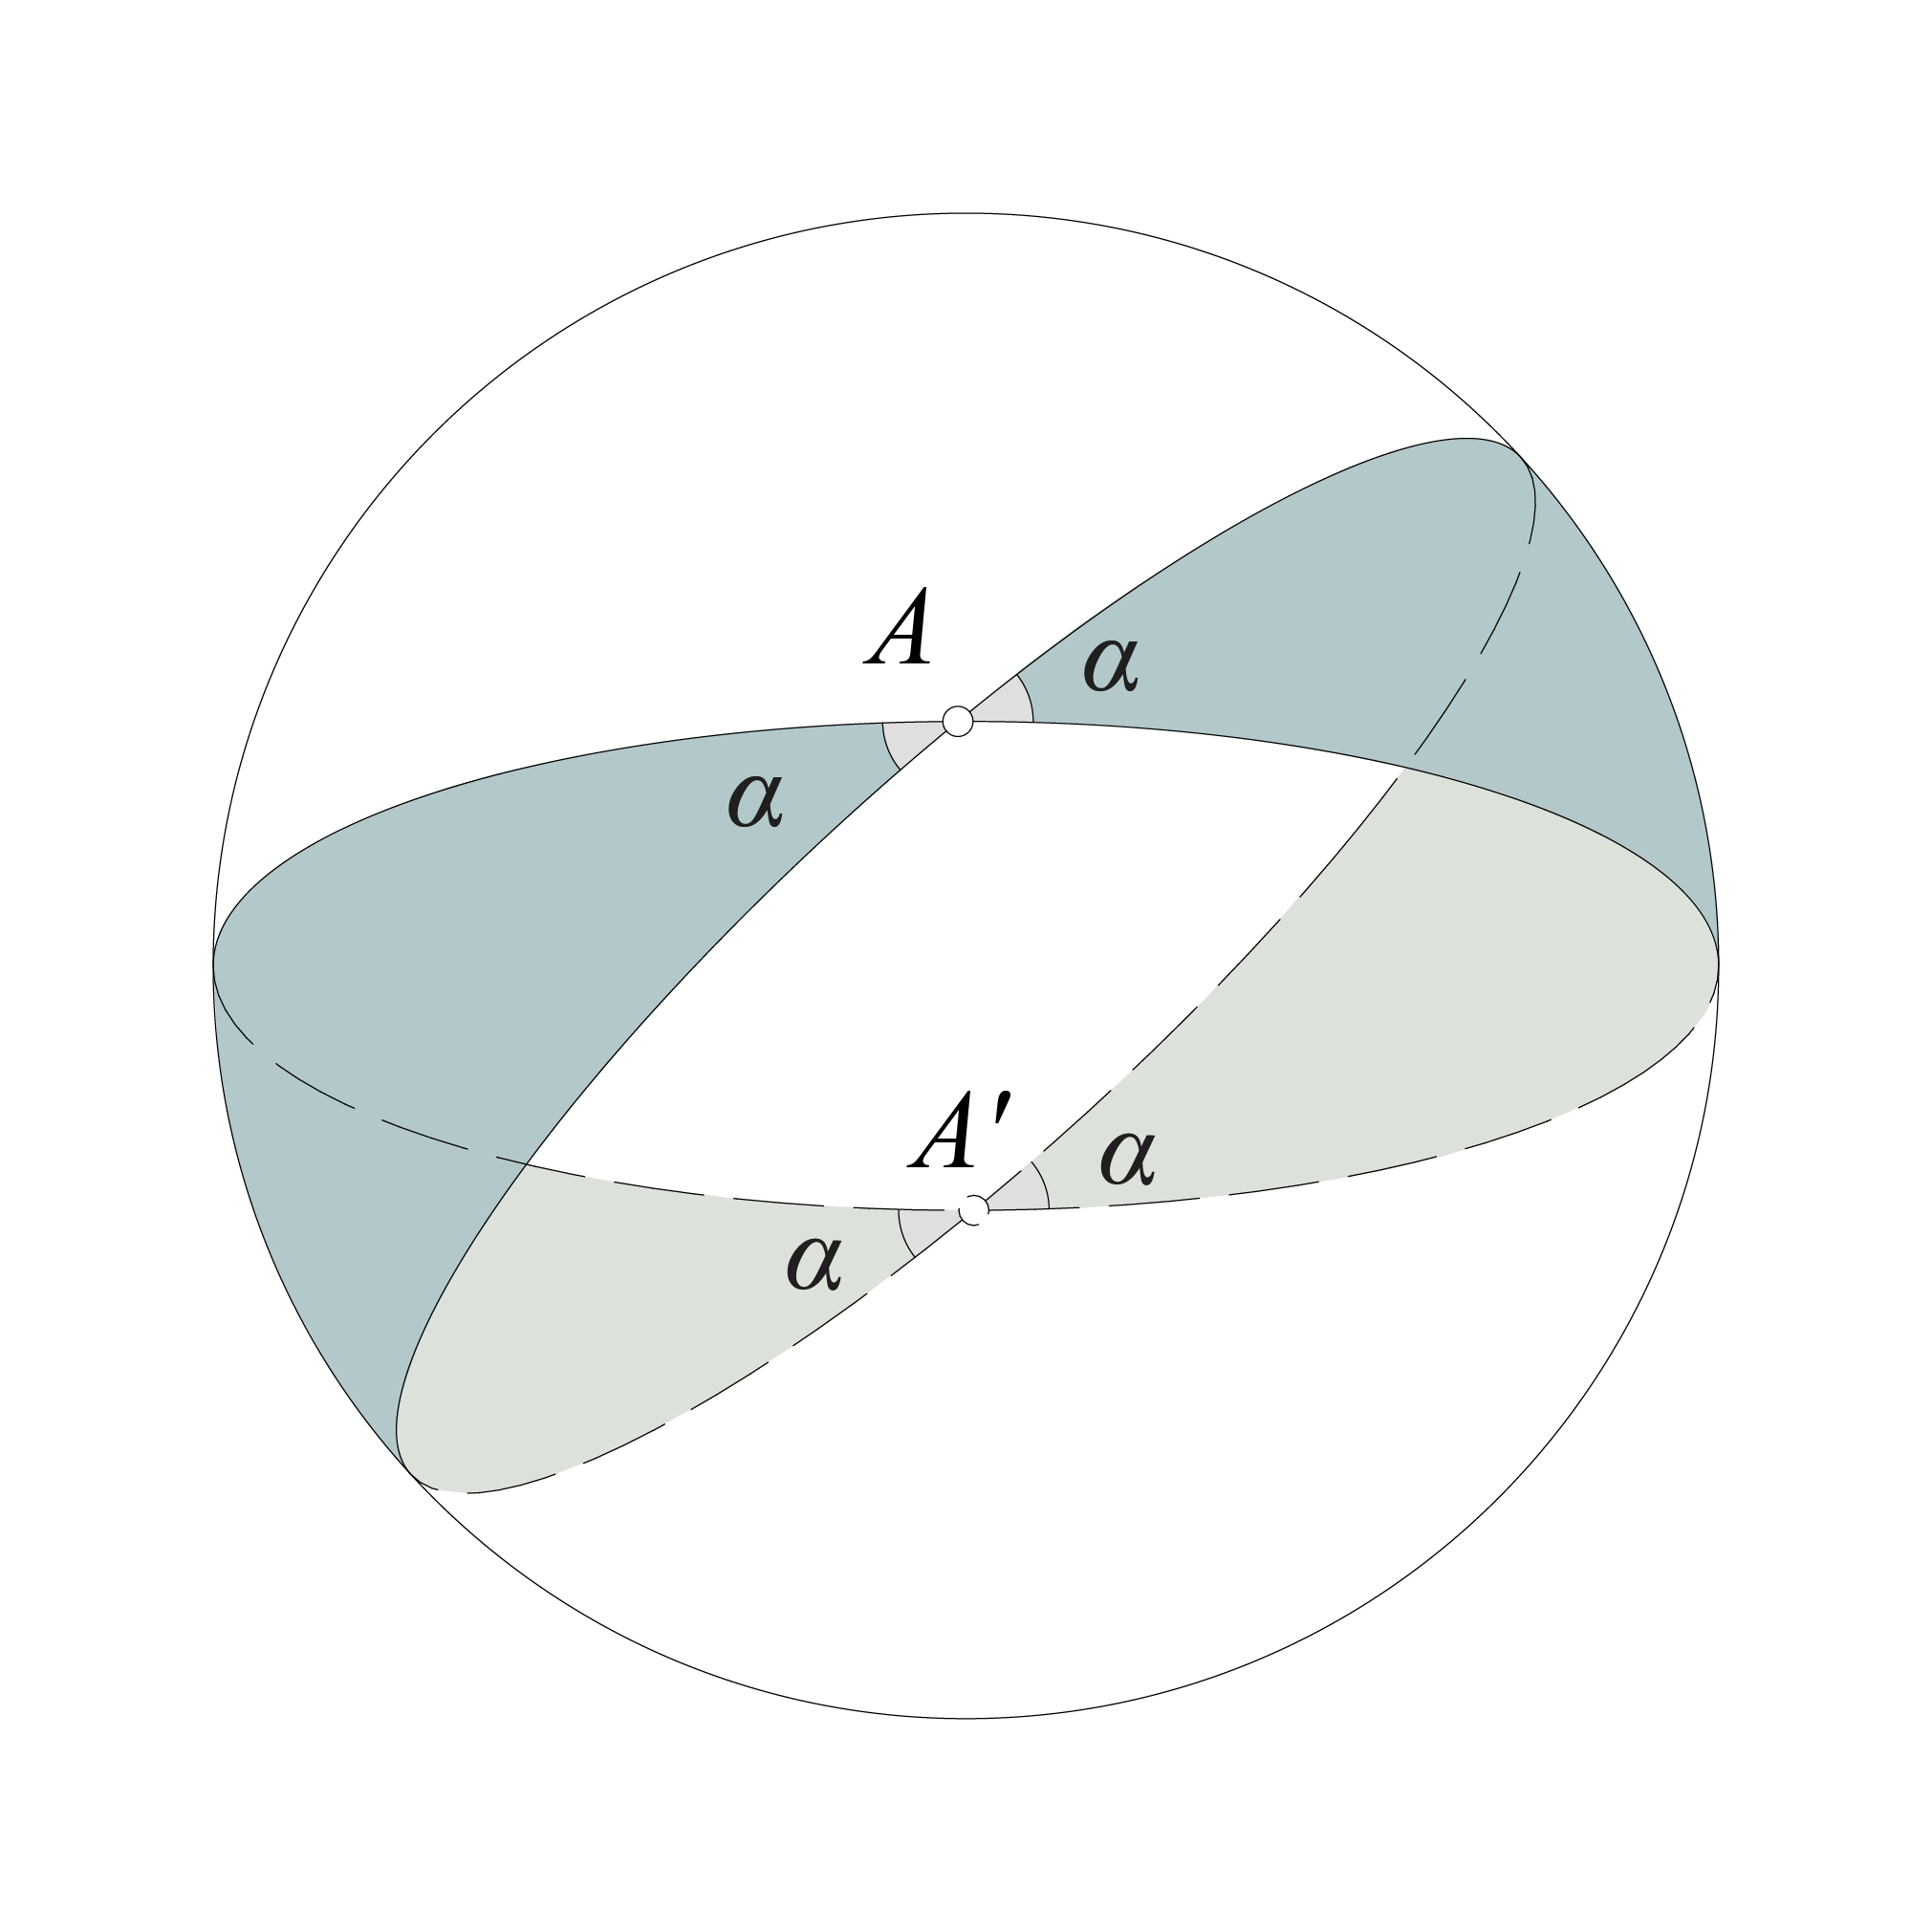
\includegraphics[width=0.4\textwidth]{kugel/Zweieck.jpg}
    \captionof{figure}{Bildung von Zweiecken durch Grosskreise}
\end{center}

Der Flächeninhalt des Zweiecks lässt sich mithilfe der Flächenformel der Kugel beschreiben

\begin{align*}
A_\text{Kugel} &= 4 \pi r^{2}
\end{align*}

Um den Flächeninhalt des Zweiecks zu erhalten, multiplizieren wir den Flächeninhalt der Kugel $A_\text{Kugel}$ mit dem des Kugelsegments des Winkels $\alpha$ 
\begin{equation}
A_\text{Zweieck} = 4 \pi r^{2} \cdot \frac{ \alpha }{ 2 \pi } = 2 \alpha r^{2}
\label {V5}
\end{equation}

Auf der Erdoberfläche finden wir Vierundzwanzig uns allbekannte Zweiecke - Die Zeitzonen. Auf dieses Thema wird im Abschnitt~\ref{Zeitzonen} \nameref{Zeitzonen} näher eingegangen.


\subsection{Eulersche Dreiecke} \label{Euler} 
Legt man drei Grosskreise auf eine Kugeloberfläche, bilden sich dabei acht Dreiecke. 
Ein solches Dreieck heisst Eulersches Dreieck\footnote{%
Leonard Euler (1707-1783), berühmter Schweizer Mathematiker und Physiker. 
Ein nicht Eulersches Dreieck erhält man, indem man das Äussere des Dreieckes ABC betrachtet.}.
Diese werden weder durch die Verlängerung ihrer Seiten durchschnitten, 
noch haben sie Dreiecksseiten, welche grösser sind als $180^{\circ}$.

\begin{center}
        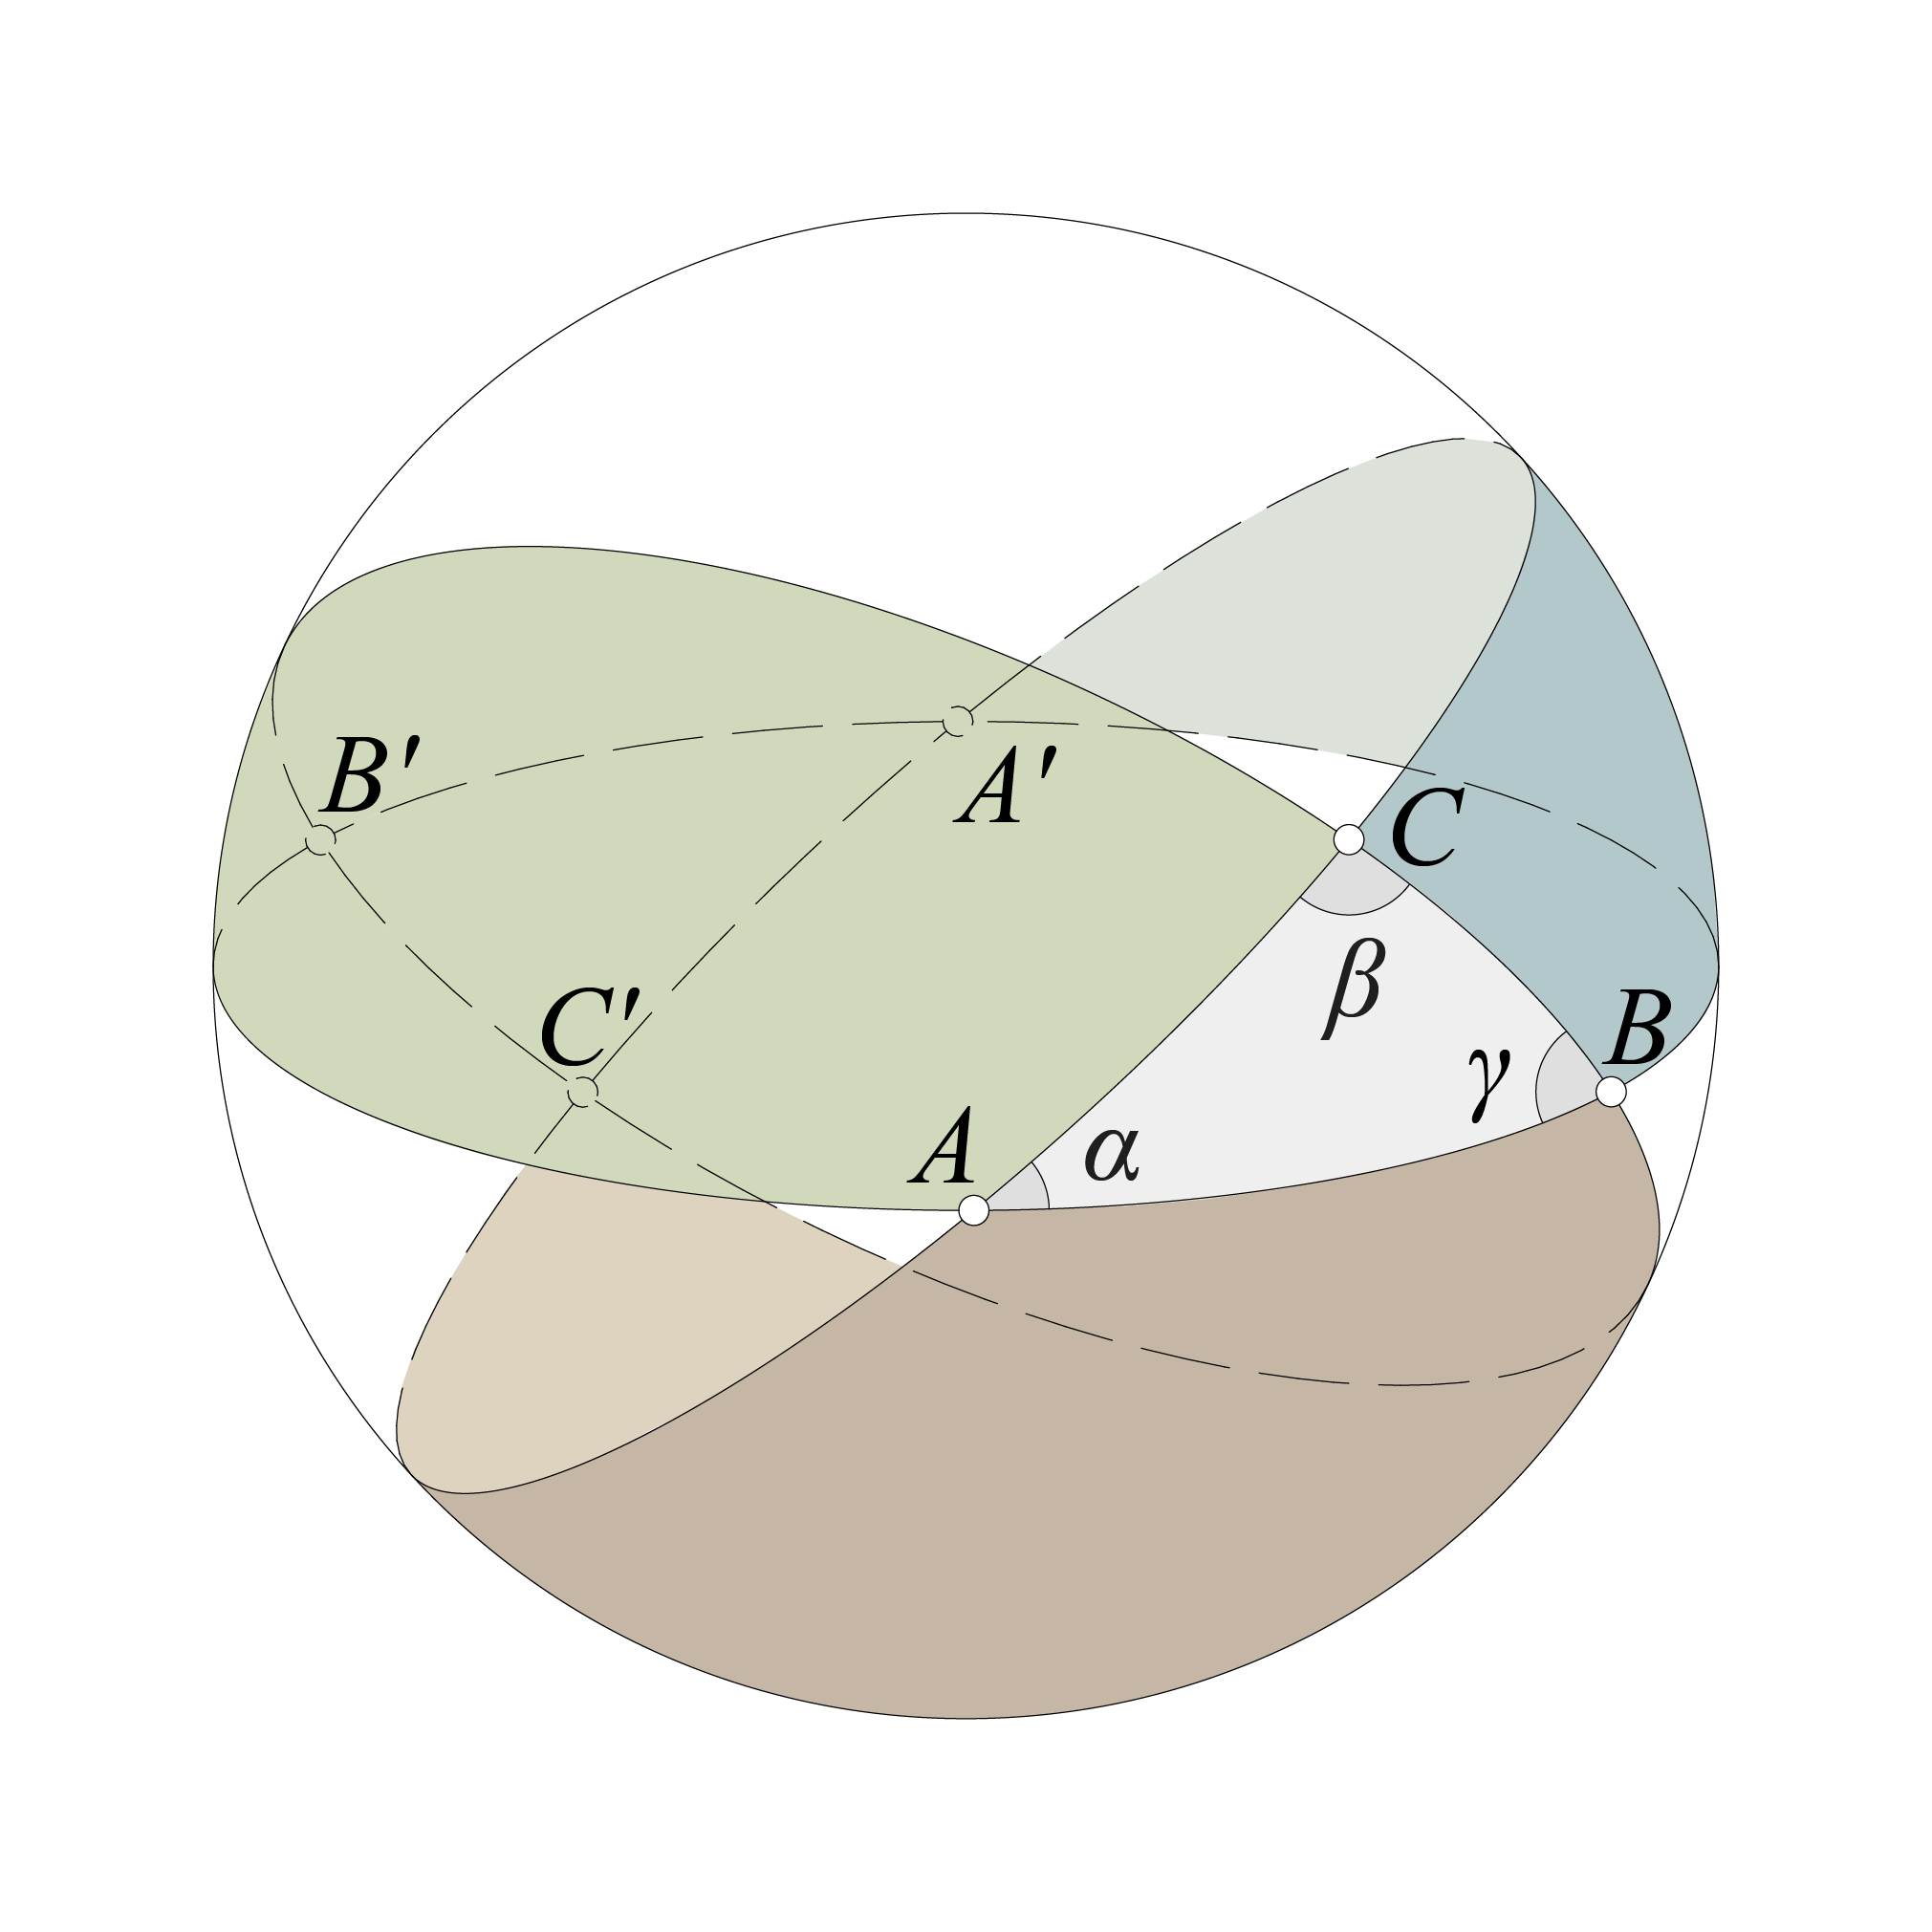
\includegraphics[width=0.4\textwidth]{kugel/EulerschesDreieck.jpg}
    \captionof{figure}{Drei Grosskreise bilden acht Eulersche Dreiecke}
\end{center}

In den nachstehenden Erklärungen und Herleitungen sprechen wir ausschliesslich von Eulerschen Dreiecken, da die umgeformten Winkelsätze der ebenen Trigonometrie nur auf diese Art von Kugeldreiecken angewendet werden können.

Aus der Ebenen Trigonometrie folgt die Formel für die Innenwinkelsumme aus dem Wechselwinkelsatz
\begin{align*}
\alpha + \beta + \gamma &= 180^{\circ}
\end{align*}

Für die Innenwinkelsumme in der sphärischen Trigonometrie gilt dies nicht. Obschon die Trigonometrie der Sphäre einige Gemeinsamkeiten zur Trigonometrie der Ebene aufweist, kann nicht alles übernommen werden.
So lässt sich auch die Innenwinkelsumme eines ebenen Dreiecks von $180^{\circ}$ in einem Eulerschen Dreieck übernehmen.
Denn diese liegt zwischen
\[
\begin{aligned}
\pi
&\text{ bis }
3\pi
&
&\text{oder}
&
180^{\circ}
&\text{ bis }
540^{\circ}
\end{aligned}
\]
Daraus können wir schliessen, das eine einzelne Seite durchaus die Grösse $180^{\circ}$ oder $\pi$ annehmen kann, jedoch nicht mehr. Ansonsten wäre es ein allgemeines Kugeldreieck und damit kein Eulersches. Dies würde wiederum bedeuten, dass wir die sphärische Trigonometrie nicht anwenden dürfen.


\subsection{Polardreieck}


\section{Dreiecksfläche und sphärischer Exzess} \label{Flaeche}
Betrachten wir das hellgraue Dreieck in der Abbildung 13.5 ist $A_{ \triangle{ ABC }}$ dessen Flächeninhalt. Dieser lässt sich aus der Summe der Winkel $\alpha$, $\beta$, $\gamma$, der Differenz $\pi$ und dem Kugelradius $r$ im Quadrat berechnen

\begin{align*}
A_{ \triangle{ ABC }} &= (\alpha + \beta + \gamma - \pi) \cdot r^2
\end{align*}

Das diese Formel zum gewünschten Flächeninhalt führt, lässt sich folgendermassen beweisen:
Als erstes berechnen wir die einzelnen Flächeninhalte der Zweiecke $A$, $B$ und $C$
\begin{align*}
\text{Zweieck A}
&=
\triangle{ABC} + \triangle{A'BC} = 2 \alpha r^{ 2 } = A_{ \alpha }\\
\text{Zweieck B}
&=
\triangle{ABC} + \triangle{AB'C} = 2 \beta r^{ 2 } = A_{ \beta }\\
\text{Zweieck C}
&=
\triangle{ABC} + \triangle{ABC’} = 2 \gamma r^{ 2 } = A_{ \gamma }
\end{align*}

Die drei Zweiecke und die beiden kleinen grauen Eulersche Dreiecke bedecken zusammen die halbe Kugel, was in der Abbildung 13.6 ersichtlich ist.

\begin{center}
        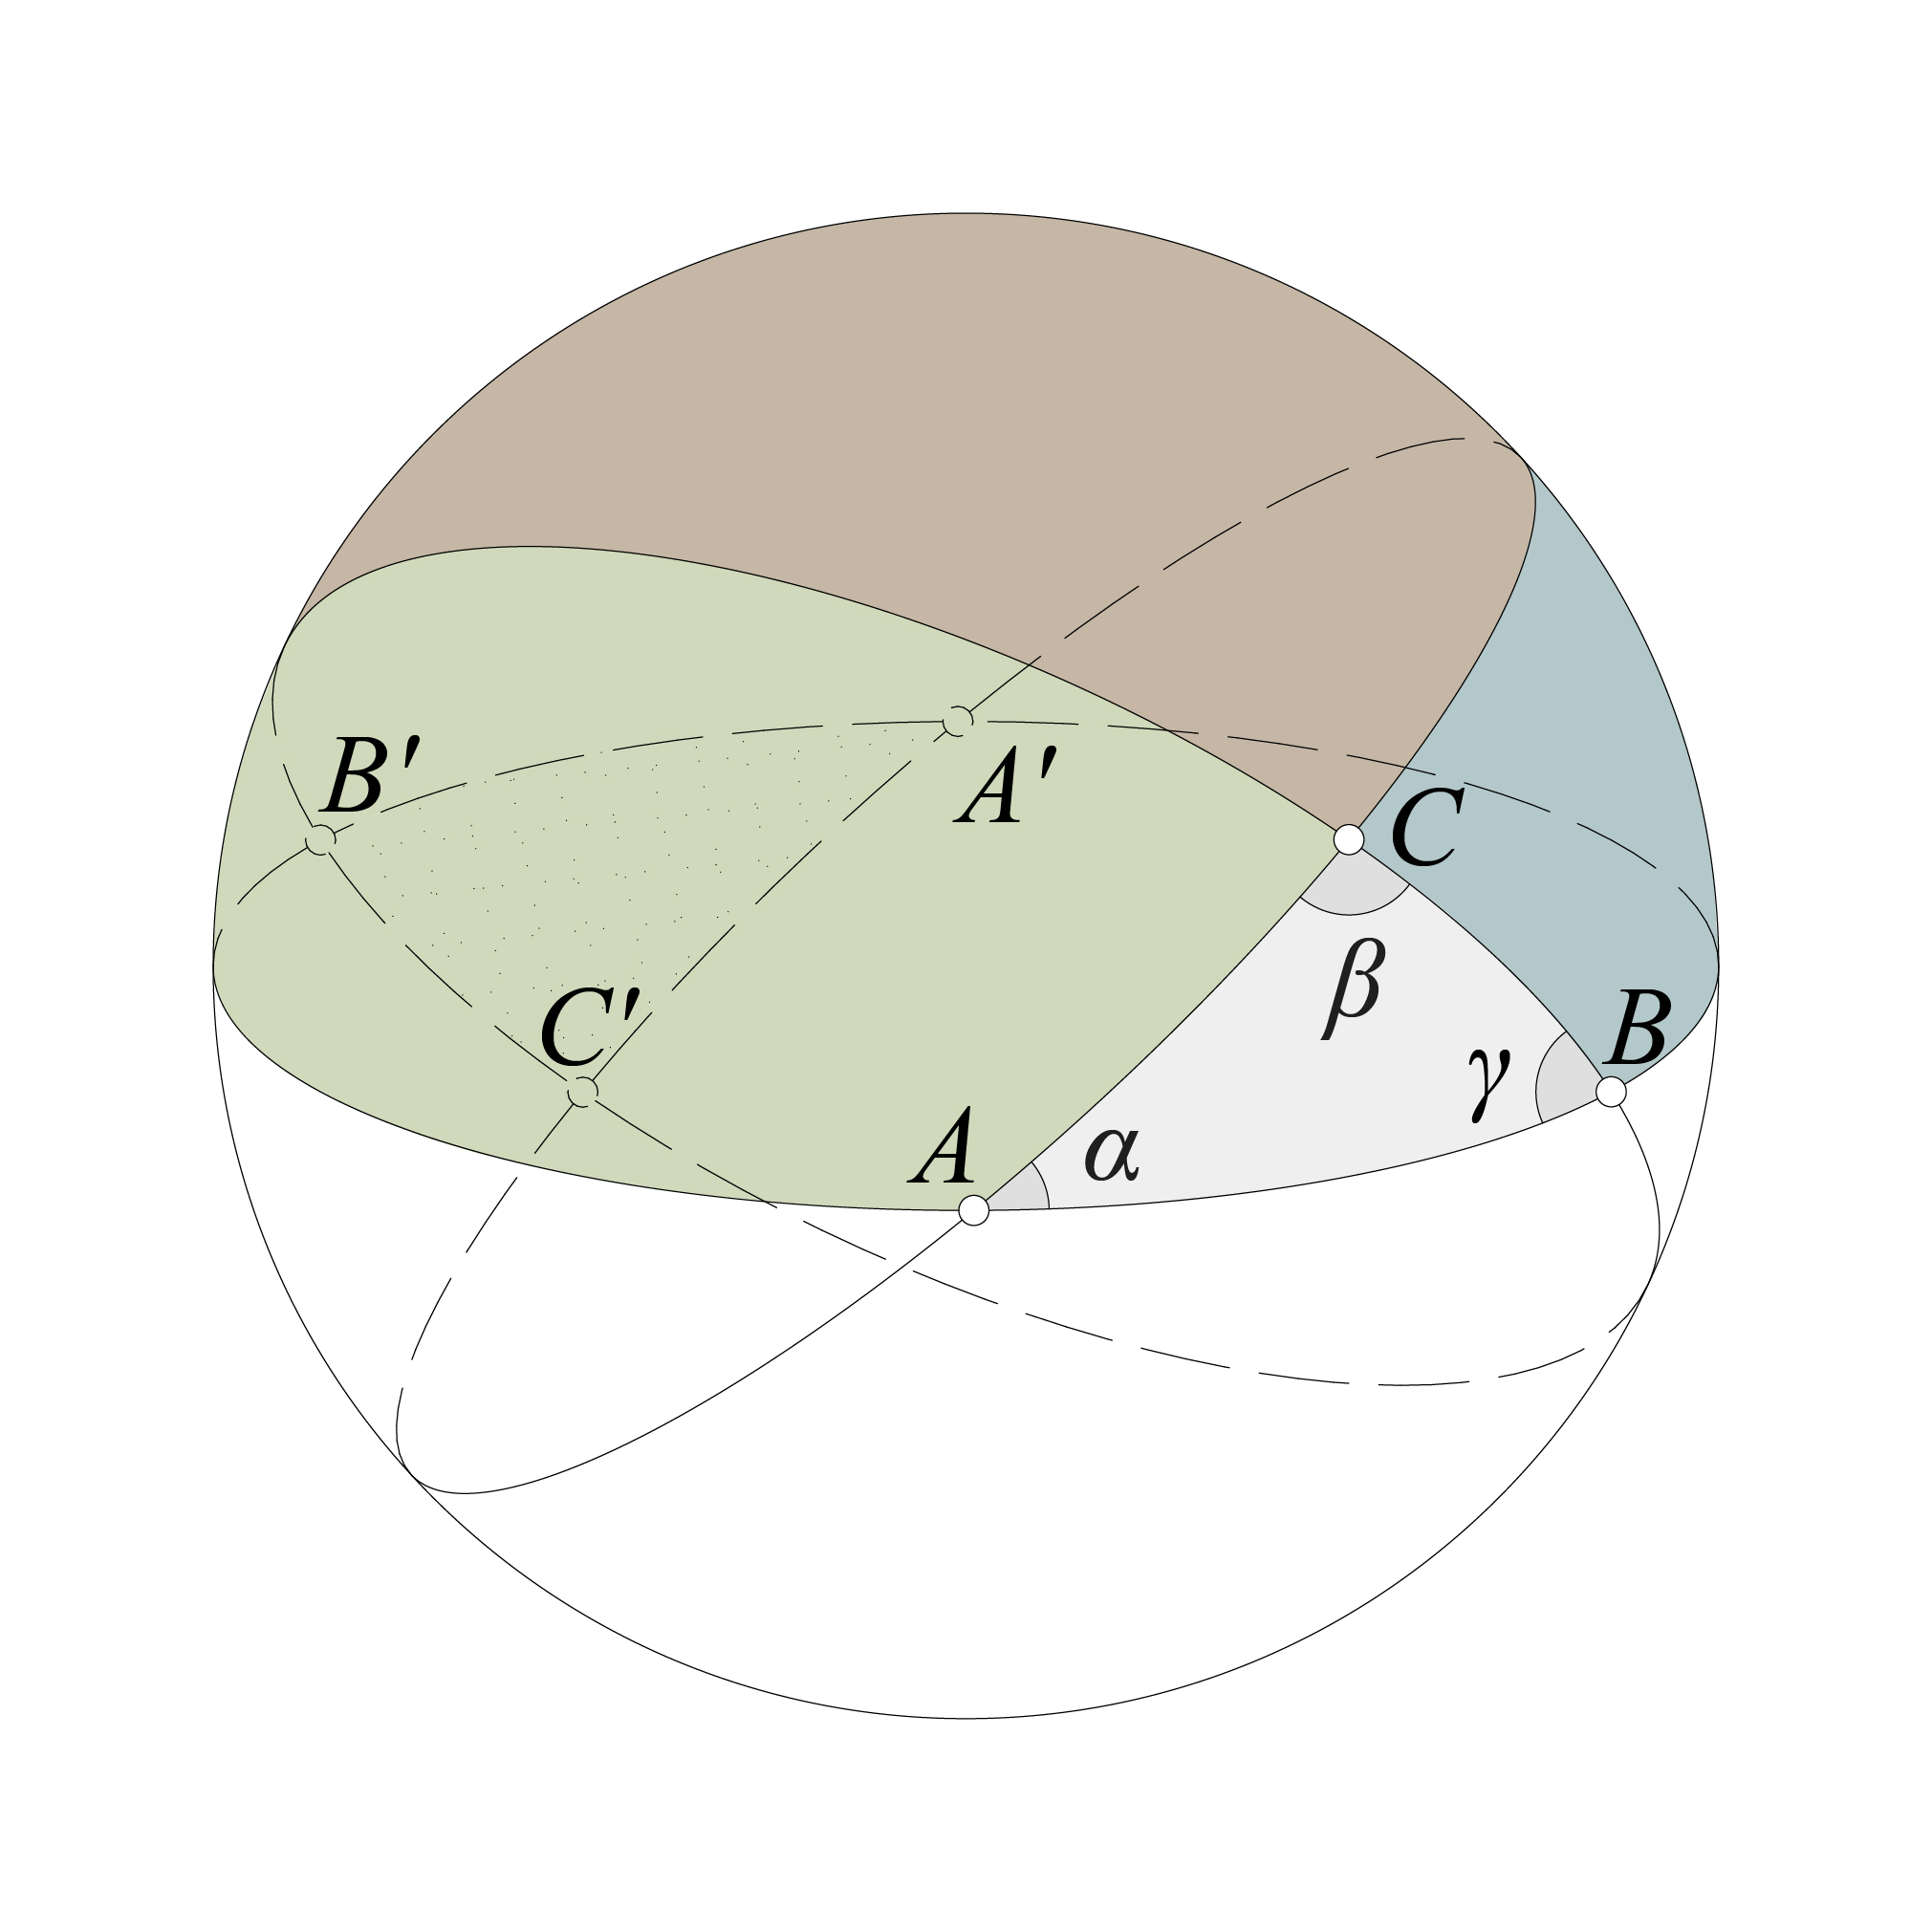
\includegraphics[width=0.4\textwidth]{kugel/HalbeKugel.jpg}
    \captionof{figure}{Die abgedeckte Halbe Kugeloberfläche durch Eulersche Dreiecke und Zweiecke}
\end{center}

Nun setzen wir die Flächeninhalte der Zweiecke mit dieser der halben Kugel gleich
\begin{align*}
A_{ \alpha } + A_{ \beta } + A_{ \gamma } &= \frac{ 4\pi r^{ 2 } }{ 2 } + 2A_{ \triangle{ ABC }}
\end{align*}

Nach der Division durch 2 Subtraktion von $\pi r^2$ schreiben wir die Formel des Flächeninhalt 
\begin{satz} \textit{Der Flächeninhalt eines Eulerschen Dreiecks verhaltet sich wie die Summe dessen Winkel subtrahiert mit $\pi$ und dessen Differenz multipliziert mit dem Radius im Quadrat.}
\label{skript:kugel:satz:Flaecheninhalt}
\index{Flaecheninhalt}
\end{satz}

\begin{align*}
A_{ \triangle{ ABC }}  &= r^{ 2 }\underbrace{(\alpha + \beta + \gamma - \pi)}_{\text{Sphärischer Exzess}}
\end{align*}

Dabei nennt die Winkelsumme, abzüglich $\pi$, den sphärischen Exzess $\epsilon$ im Kugeldreieck.
$\epsilon$ gibt die Abweichung von $\pi$ an, die Differenz ist der sphärische Exzess und tritt nur in Dreiecken auf der Kugel auf. 
Dies hat mit der gekrümmten Oberfläche der Kugel zu tun.
\begin{equation}
\epsilon = \alpha + \beta + \gamma - \pi
\end{equation}


\begin{center}
        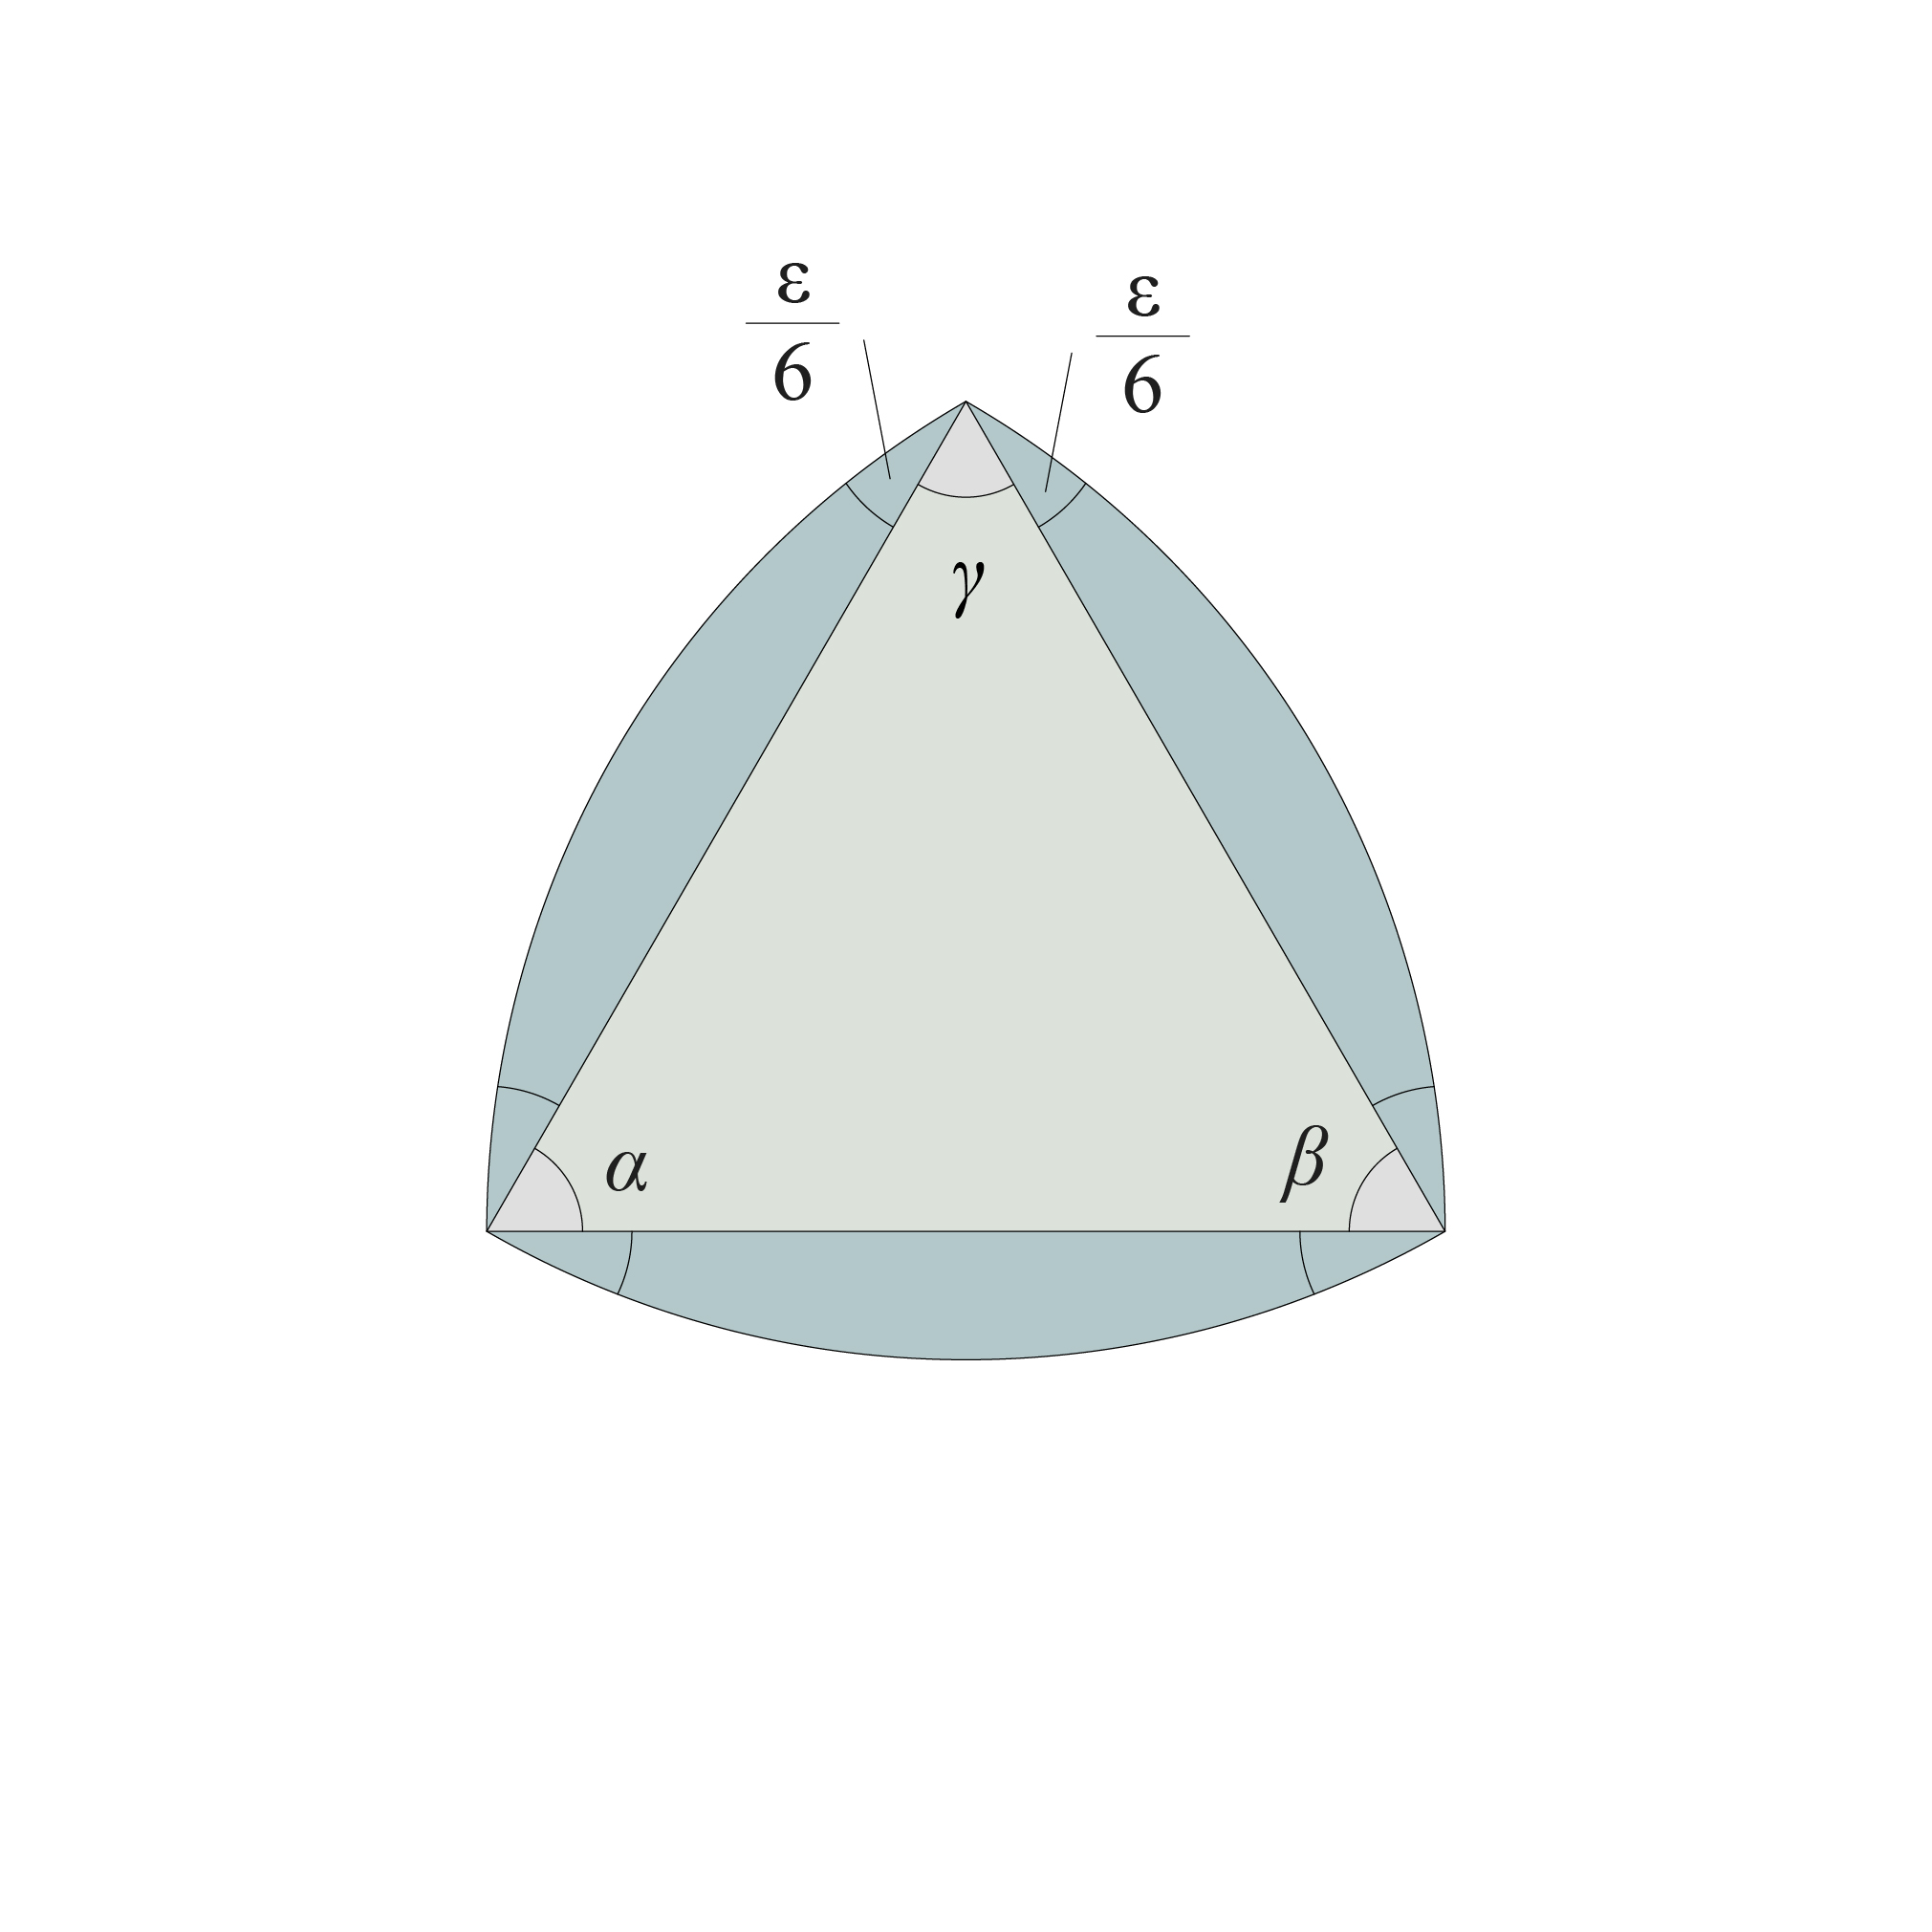
\includegraphics[width=0.5\textwidth]{kugel/SphaerischerExzess.jpg}
    \captionof{figure}{Sphärischer Exzess bei einem Gleichseitigen Dreieck}
\end{center}

Folglich ist der Exzess direkt mit dem Flächeninhalt $\triangle A$ eines Eulerschen Dreiecks verbunden
\begin{align*}
\epsilon =\frac{A_{\triangle{ ABC }}}{r^2} = \frac{\alpha + \beta + \gamma - \pi}{r^2}
\end{align*}

Ist der sphärische Exzess und der Flächeninhalt bekannt, kann man mit dessen Hilfe auf einem beliebigen Eulerschen Dreieck auf dessen Radius
\begin{align*}
r = \sqrt{\frac{\alpha + \beta + \gamma - \pi}{\epsilon}}
\end{align*}

schliessen. Mit einer maximalen Innenwinkelsumme bei Eulerschen Dreiecken von $540^{\circ}$ ist der Exzess maximal $360^{\circ}$.
\[
\begin{aligned}
0^{\circ} \le \epsilon \le 360^{\circ}
&
&\text{oder}
&
&\pi \le \epsilon \le 2\pi
\end{aligned}
\]

Berechnen wir den maximalen sphärischen Exzess bei allgemeinen Kugeldreiecken würde dieser maximal $720^{\circ}$ annehmen.
\[
\begin{aligned}
0^{\circ} \le \epsilon \le 720^{\circ}
&
&\text{oder}
&
&\pi \le \epsilon \le 4\pi
\end{aligned}
\]



\subsection{Grenzfall - Satz von Legendre}
Würden wir den sphärischen Exzess in der ebenen Trigonometrie anwenden, wäre dieser $=0$. Betrachten wir nun sehr kleine Kugeldreiecke oder mit grossen aber endlichen Radien, würde die Innenwinkelsumme $\pi$ nur wenig übersteigen. Dies besagt, dass wir sphärische Dreiecke mit geringer Grösse durch „Verebnung“ annähernd als solche der ebenen Trigonometrie betrachten können. Diese Erkenntnis beschreibt der Satz von Legendre

\begin{center}
        \includegraphics[width=0.4\textwidth]{kugel/Beispielbild.jpg}
    \captionof{figure}{Bild Krümmung Gross und Klein}
\end{center}

\begin{quote} \textit{Ein kleines sphärisches Dreieck kann näherungsweise 
wie ein ebenes Dreieck mit denselben Seiten berechnet 
werden, wenn alle Winkel des ebenen Dreiecks die um 
je ein Drittel des sphärischen Exzesses verminderten 
Winkel des sphärischen Dreiecks nimmt.} \end{quote}
\begin{flushright} - Adrien-Marie Legendre (1752-1833), Paris 1787
\end{flushright}

Durch diesen Satz lässt sich der Zusammenhang zwischen der Ebenen Trigonometrie und der Trigonometrie auf der Kugel herstellen.



\section{Sphärisch Analoge Winkelfunktionen}
Euklid von Alexandria\footnote{%
Euklid war ein griechischer Mathematiker. Er lebte wahrscheinlich 3 Jahrhunderte vor Christus. In seinem berühmtesten Werk \textit{Euklids Elemente} fasst er die Arithmetik und Geometrie seiner Zeit zusammen. \textit{Euklids Elemente} war 2000 Jahre lang als Lehrbuch in gebrauch und war bis Mitte des 19. Jahrhunderts nach der Bibel das weit verbreitetste Buch der Weltliteratur.}  beschrieb die Grundbegriffe der ebenen Geometrie mittels Punkt, Gerade, Ebene, Winkel und Dreieck. Ebendiese Dreiecke lassen sich mithilfe der ebenen Trigonometrie beschreiben. Dabei gelten die uns bekannten trigonometrischen Winkelfunktionen:

Der Sinussatz
\begin{align*}
\frac{ a }{\sin(\alpha) } &= \frac{ b }{\sin(\beta)} = \frac{ c }{\sin(\gamma)}
\end{align*}
welcher nichts anderes ist als der Strahlensatz des ebenen Dreiecks. Das Verhältnis der Längen zweier Seiten ist gleich dem Verhältnis der Sinuswerte der gegenüberliegenden Winkel.

Und der Cosinussatz
\begin{align*}
c^{ 2 } &= a^{ 2 } + b^{ 2 } - 2ab\cdot \cos(\gamma)\\
b^{ 2 } &= a^{ 2 } + c^{ 2 } - 2ab\cdot \cos(\beta)\\
a^{ 2 } &= b^{ 2 } + c^{ 2 } - 2ab\cdot \cos(\alpha)
\end{align*}
welcher Beziehungen zwischen den Seiten und den Kosinuswerten der Winkel im Dreieck der Ebene aufstellt.

Um diese Winkelfunktionen auf der Kugeloberfläche anwenden zu können, benötigen wir die sphärische Trigonometrie. Die oben beschriebenen Sätze lassen sich auf der Kugel nicht anwenden, sie werden aber als Grundlage und Gedankenstütze zur Herleitung der Sätze für das Kugeldreieck benötigt.



\subsection{Sphärischer Sinussatz}
Wir betrachten das folgende sphärische Dreieck auf einem Teilstück der Kugeloberfläche mit dem Radius $R= \overline{MA} = \overline{MB} = \overline{MC}$. Wir fügen ein ebenes Dreieck $\triangle=\overline{ADE}$ in das Kugelstück ein, welches den Eckpunkt $A$ beinhaltet und eine Abbildung des sphärischen Dreieckes bildet.

\begin{center}
        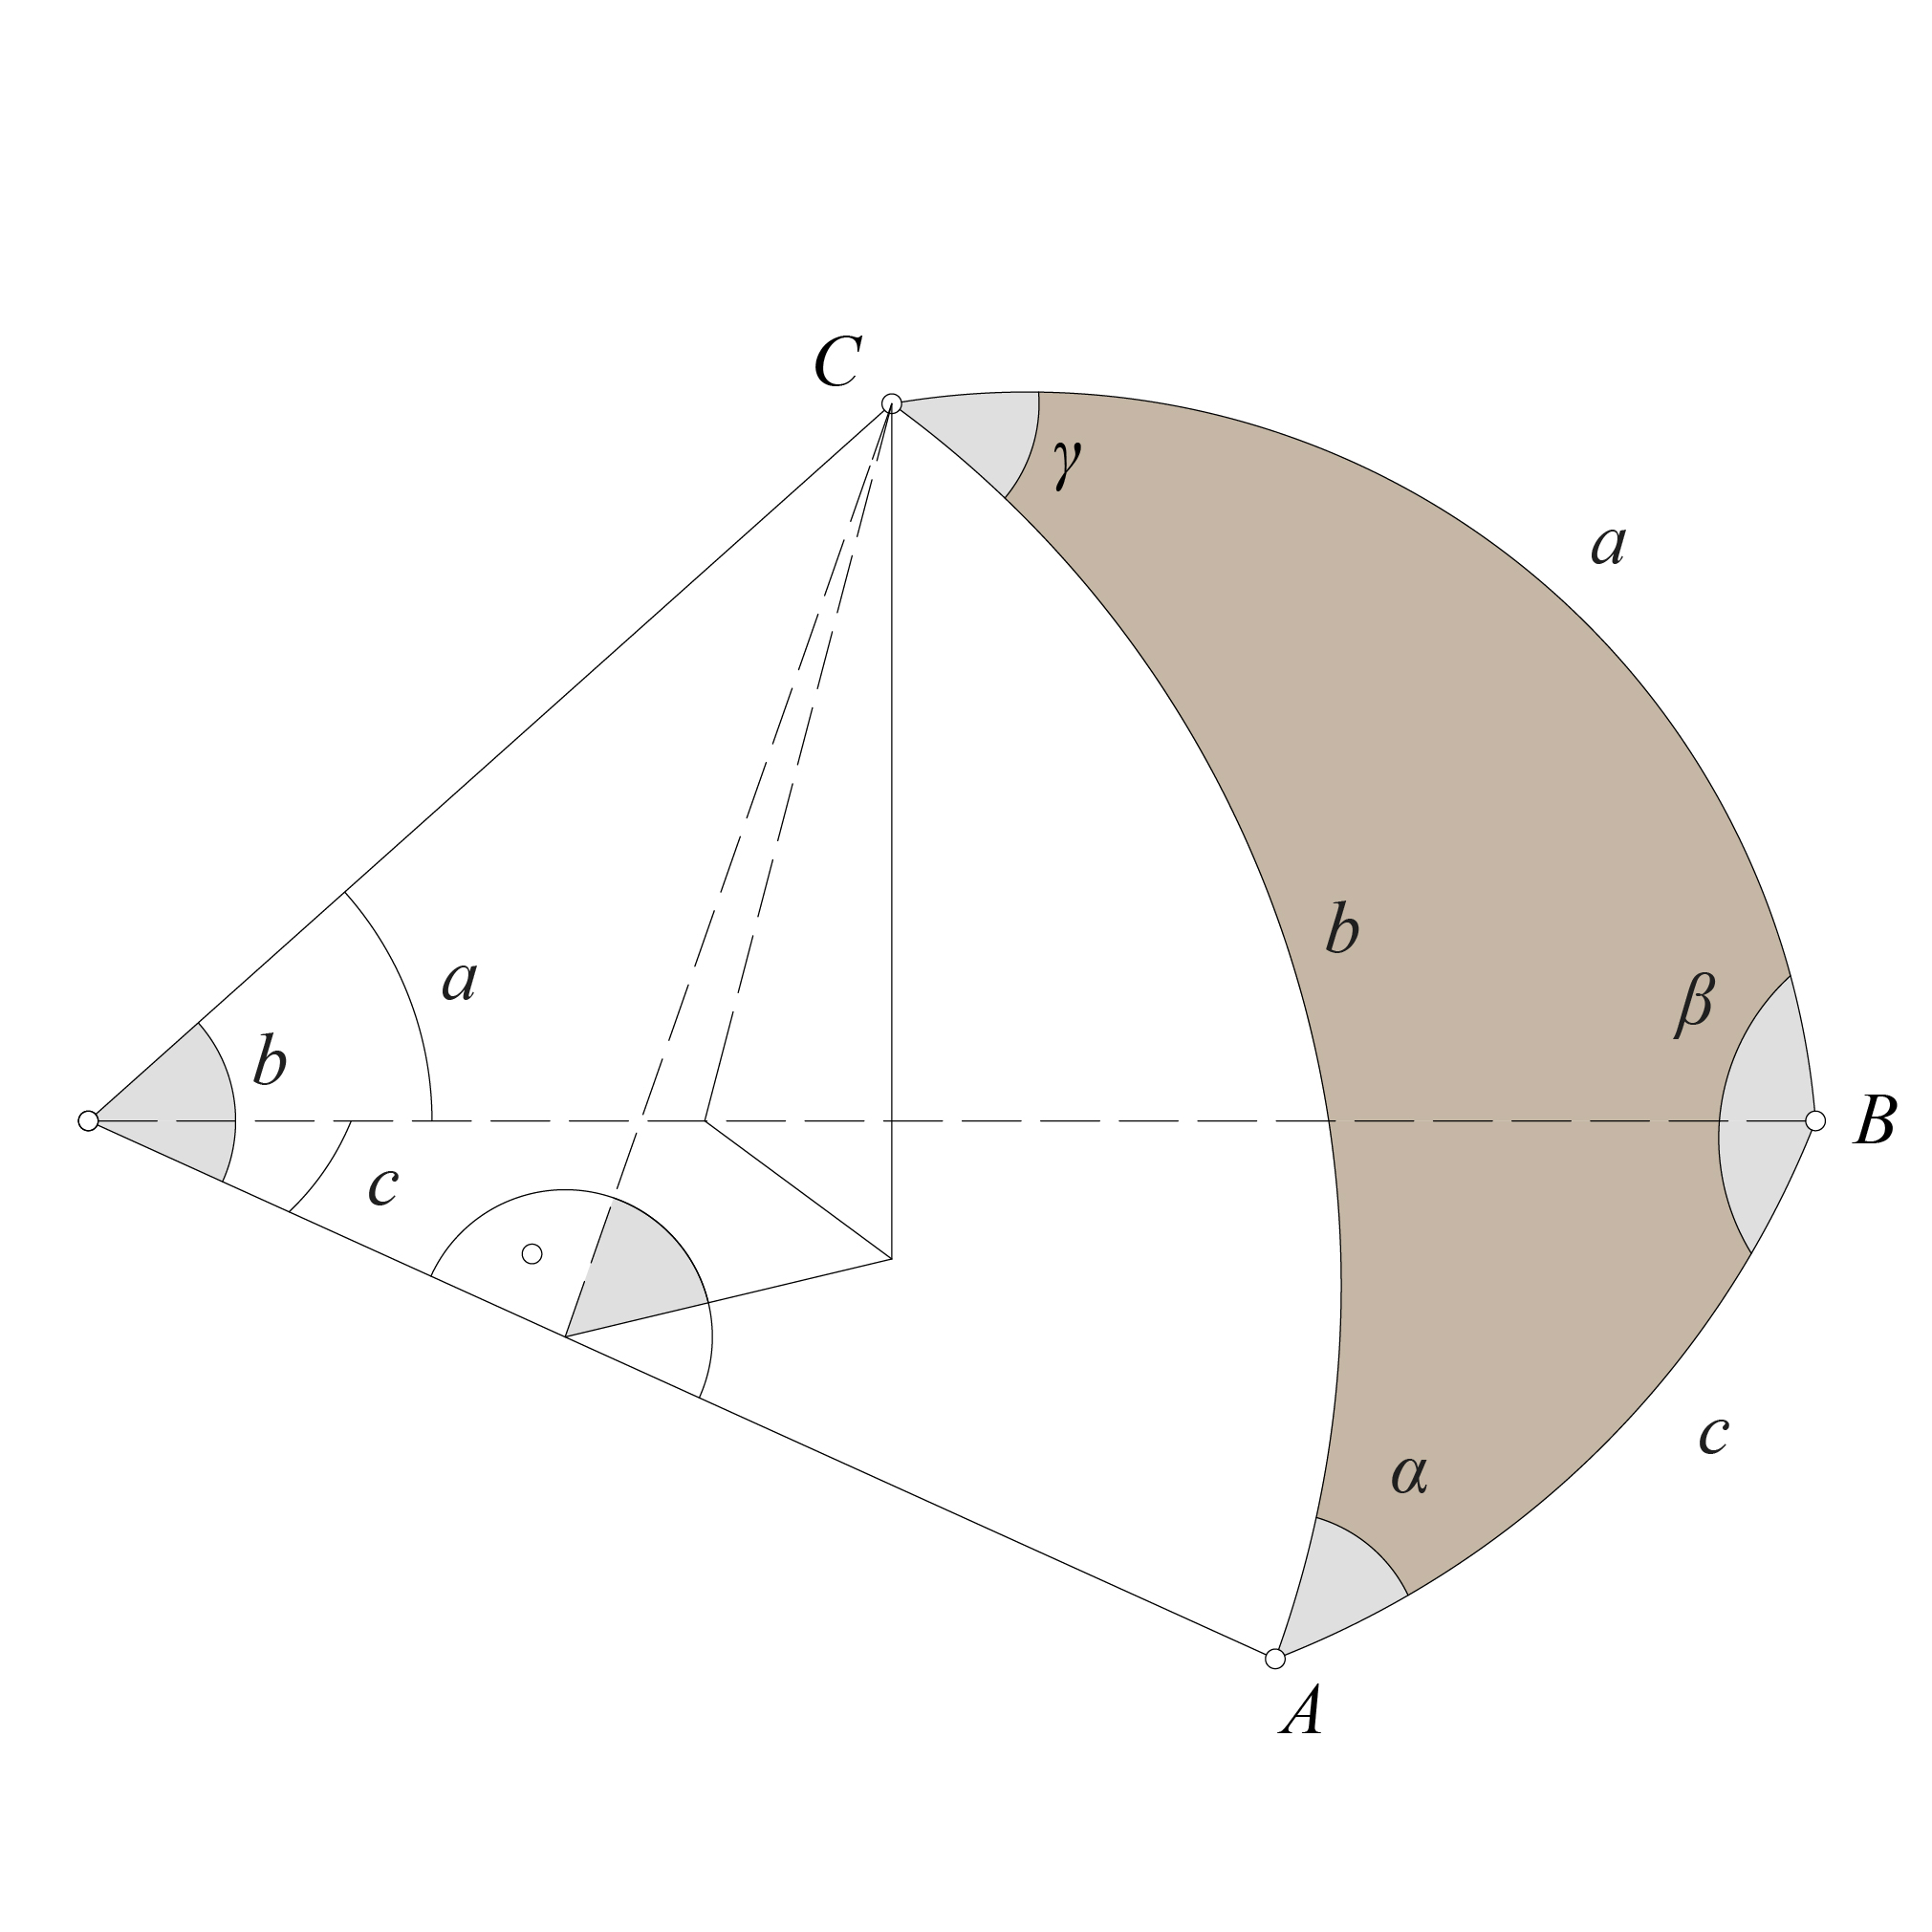
\includegraphics[width=0.6\textwidth]{kugel/Sinussatz.jpg}
    \captionof{figure}{Bild Sinussatz}
\end{center}

Es gilt

\begin{align*}
\overline{AD} &= R \cdot \sin (c)
\end{align*}

Diese Strecke ist kongruent zur Strecke
\begin{align}
h_{A} = \overline{AF} &= \overline{AD} \cdot \sin(\beta) = R \cdot \sin(c) \cdot \sin(\beta)  
\label {V1}
\end{align}

Aus einer anderen Sichtweise lässt sich die Strecke wie folgt schreiben
\begin{align}
h_{A} = R \cdot \sin(b) \cdot \sin(\gamma)  
\label {V2}
\end{align}

Durch gleichsetzen der Ausdrücke \eqref{V1} und \eqref{V2} eliminieren wir den Faktor $R$ und es entsteht der Ausdruck
\begin{align*}
\sin(c) \cdot \sin(\beta) &= \sin(b) \cdot \sin(\gamma) \\
\Rightarrow \quad \quad
\frac{\sin (b)}{\sin (c)} &= \frac{\sin (\beta)}{\sin (\gamma)}
\end{align*}

Analog dazu könnte man auch die Höhe $h_{B}$ nehmen und würde erhalten
\begin{align*}
\sin(c) \cdot \sin(\alpha) &= \sin(a) \cdot \sin(\gamma) \\
\Rightarrow \quad \quad
\frac{\sin (a)}{\sin (c)} &= \frac{\sin (\alpha)}{\sin (\gamma)}
\end{align*}

Aus diesen Erkenntnissen lässt sich der Sinussatz zusammenfassen
\begin{satz}\textit{Die Sinuswerte der Seiten verhalten sich wie die Sinuswerte der gegenüberliegenden Winkel.}
\label{skript:kugel:satz:Sinussatz}
\index{Sinussatz}
\end{satz}

\begin{align*}
\sin a : \sin b : \sin c &= \sin \alpha : \sin \beta : \sin \gamma \\
\text{oder}
\frac{\sin \alpha} {\sin a} &= \frac{\sin \beta} {\sin b} = \frac{\sin \gamma} {\sin c}
\end{align*} 

Es fällt auf, das der Satz sehr ähnlich ist zur Ebenen Trigonometrie. Der Grund weshalb man auch bei den Seiten den Sinuswert nehmen muss ist folgender:

Das Verhältnis zwischen den Seiten und Winkeln wird nicht unendlich lange grösser je weiter man sich vom gesuchten Winkel entfernt. Auf der Kugel steigt der Wert nur bis in die Mitte des Zweiecks an, dort angelangt sinkt das Verhältnis wieder solange, bis es beim Eckpunkt $A’$ angekommen ist.

\begin{center}
        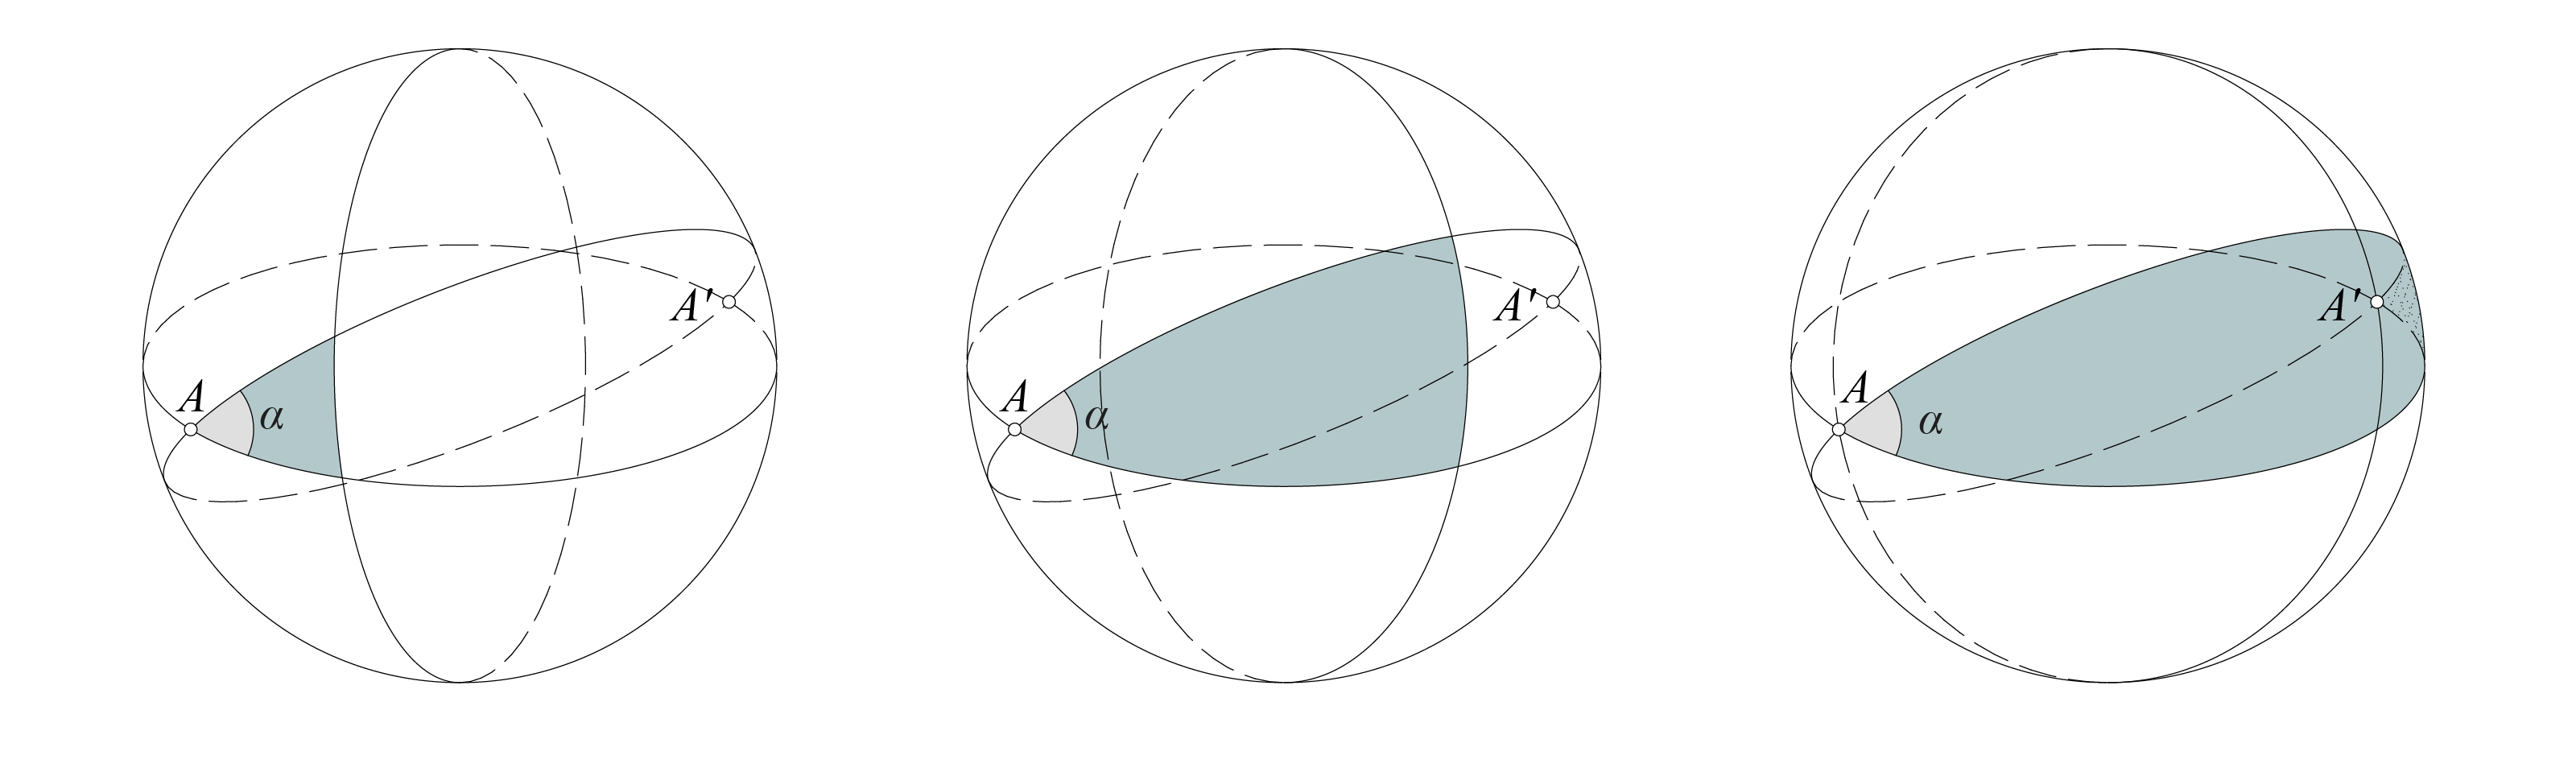
\includegraphics[width=0.9\textwidth]{kugel/SinussatzB.jpg}
    \captionof{figure}{Bild Sinussatz}
\end{center}

\subsection{Seitenkosinussatz}
Es sei das Stück einer Kugel mit dem sphärischen Dreieck $ABC$ und den Winkeln $\alpha, \beta, \gamma$ und den Seiten $a, b, c$. Die Senkrechten durch den Mittelpunkt schneiden dabei die Eckpunkte des sphärischen Dreieckes. Wir erstellen in der Ebene ein ähnliches Dreieck $A’B’C’$.

\begin{center}
        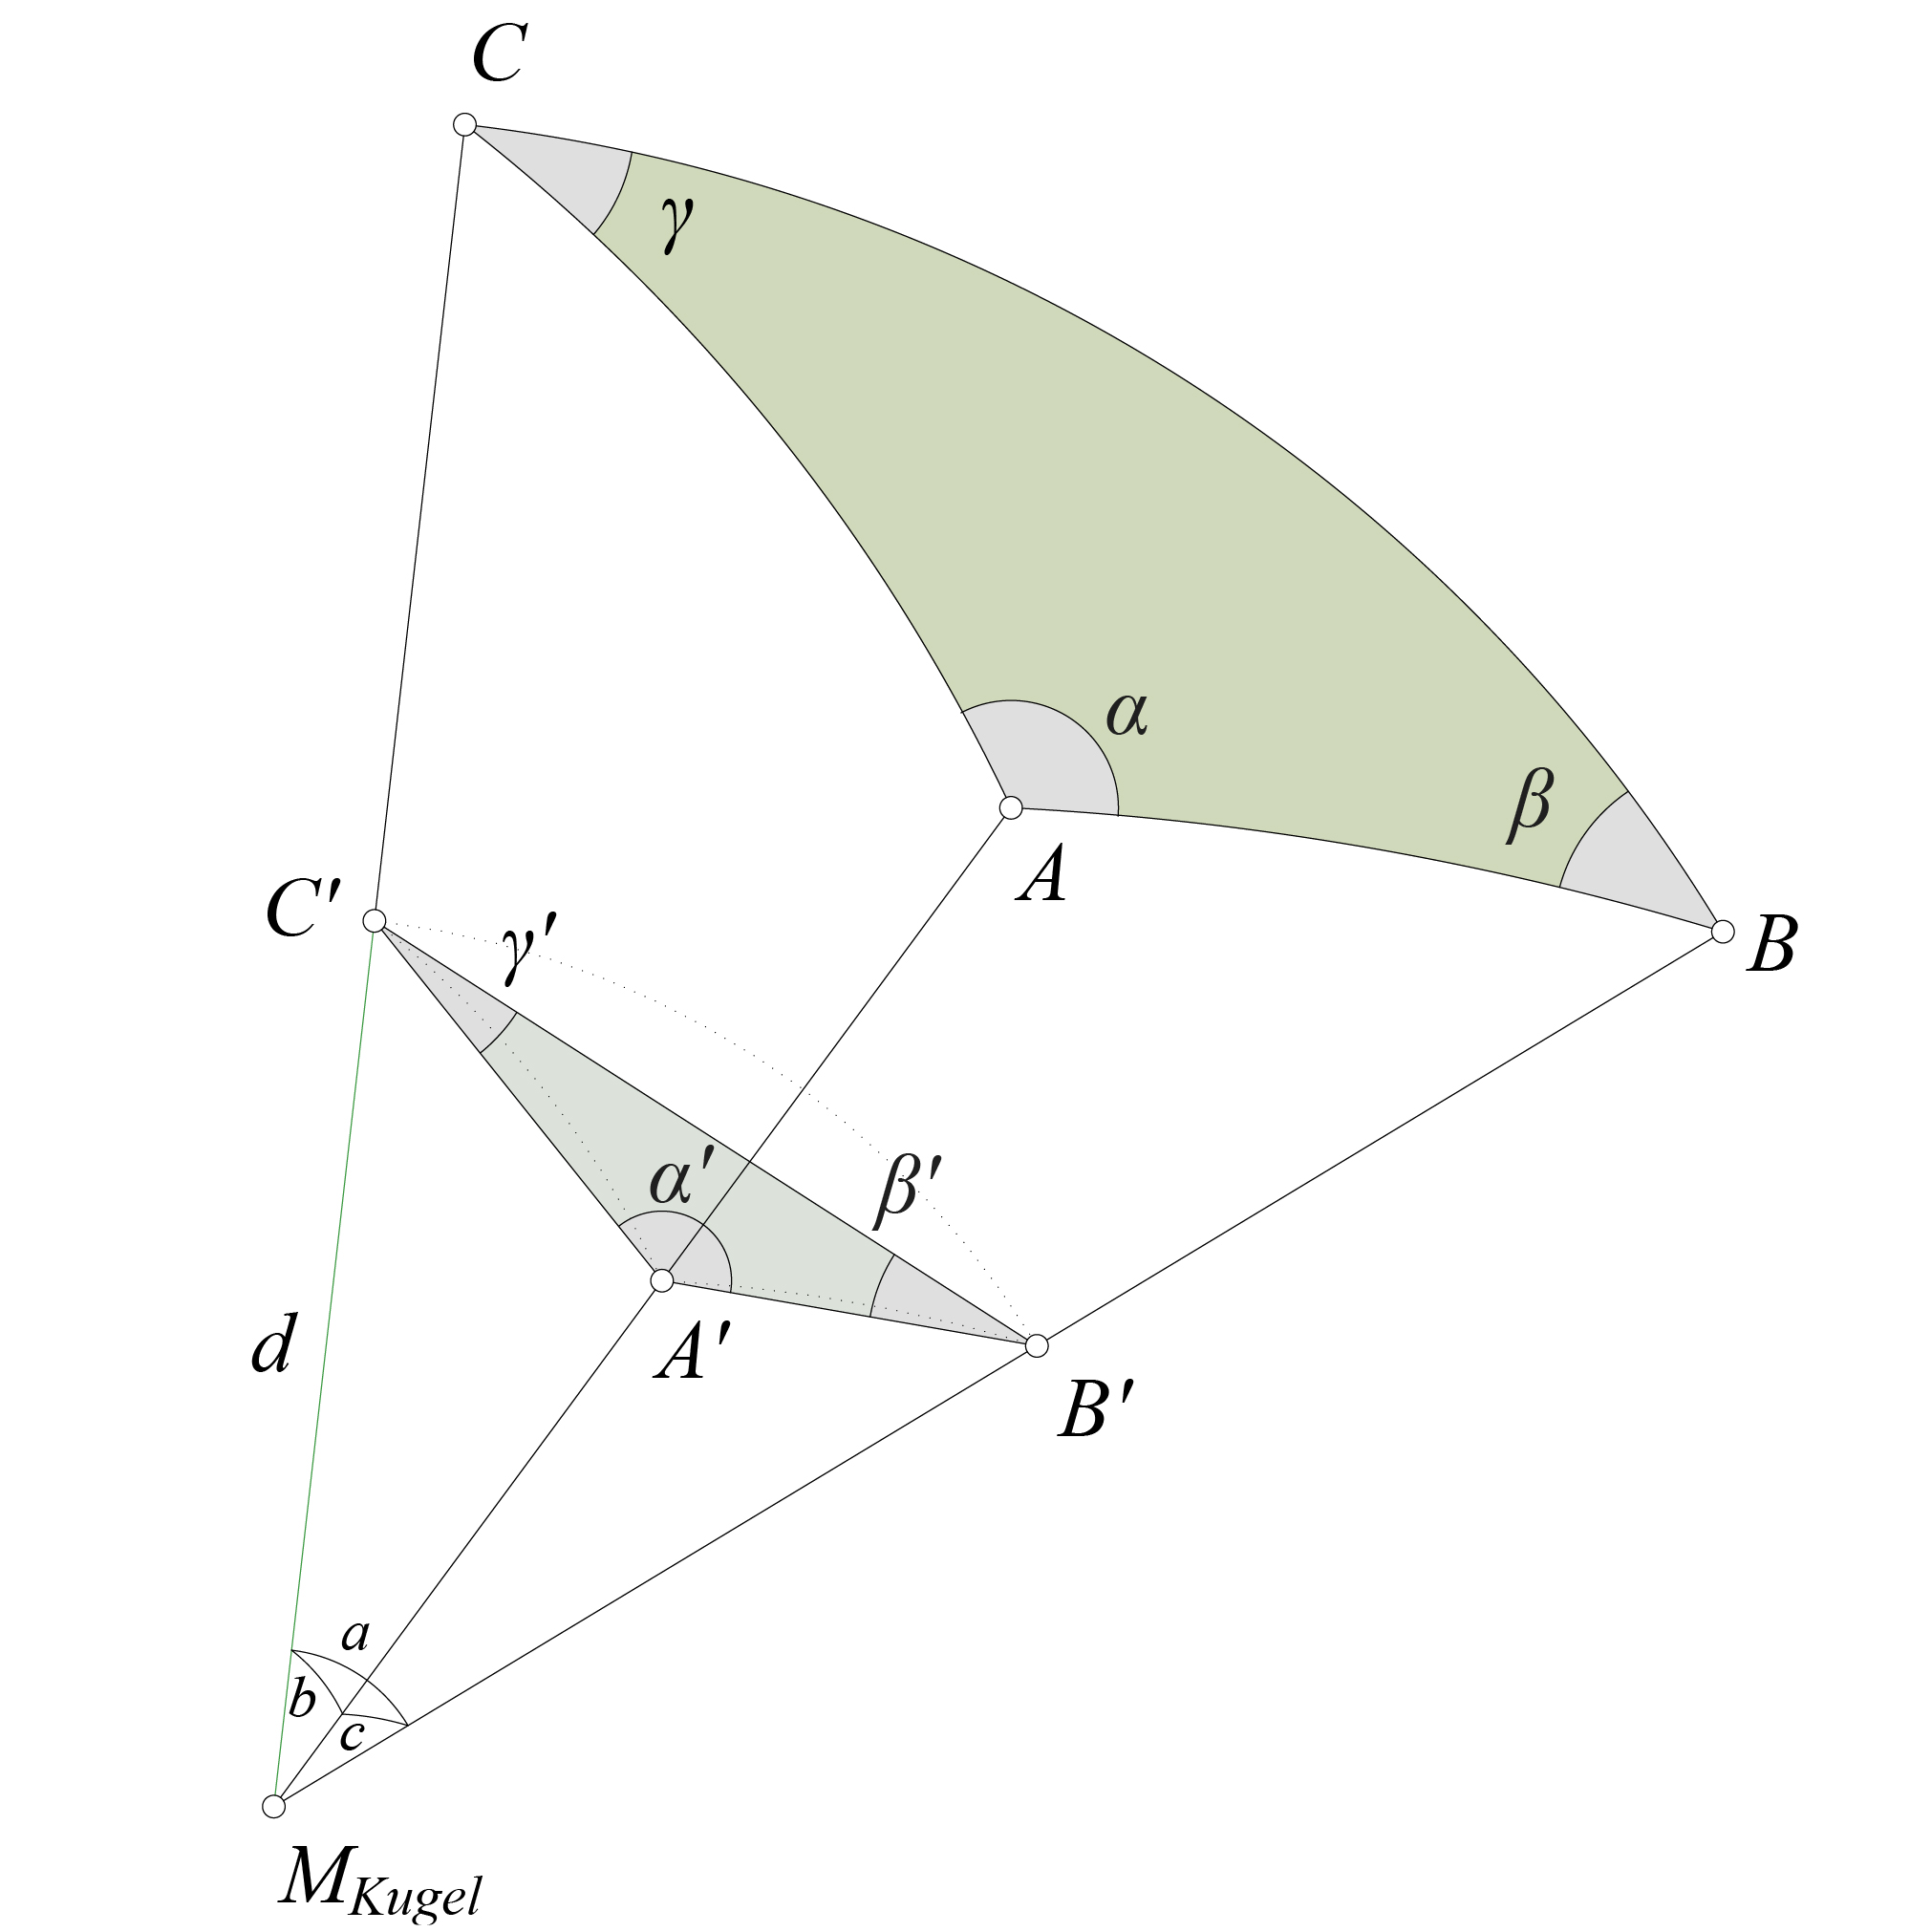
\includegraphics[width=0.4\textwidth]{kugel/Seitenkosinus.jpg}
    \captionof{figure}{Bild Seitenkosinus}
\end{center}

Die Strecken lassen sich nach den bekannten Regeln der Trigonometrie beschreiben:
\begin{align*}
\overline{C'A'} = d\cdot {\tan(b)} \quad \quad \quad \quad \quad \quad 
\overline{MA'} = \frac{ d }{\cos(b)} \\
\overline{C'B'} = d\cdot {\tan(a)} \quad \quad \quad \quad \quad \quad 
\overline{MB'} = \frac{ d }{\cos(a)}
\end{align*} 


Durch Anwenden des Kosinussatzes der Ebene auf das Dreieck $A’B’C’$ erhalten wir
\begin{align}
\overline{A'B'}^{ 2 } &= \overline{ C'B' }^{ 2 } + \overline{ C'A' }^{ 2 } - 2 \cdot \overline{C'B'} \cdot \overline{ C'A' } \cdot cos(\gamma) \nonumber \\ 
\Rightarrow \quad \quad
\overline{A'B'}^{ 2 } &= d^{ 2 } \cdot \left(\left(tan^{ 2 }(a) + tan^{ 2 }(b)\right) - 2\cdot tan(a) \cdot \tan(b) \cdot cos(\gamma)\right) 
\label {V3} 
\end{align}

Dies gilt ebenso für das Dreieck $MA’B’$
\begin{align*}
\overline{A'B'}^{2} &= \overline{MB'}^{2} + \overline{MA'}^{2} - 2\cdot \overline{MB'} \cdot \overline{MA'} \cdot \cos(c)
\end{align*}

\begin{align}
\Rightarrow \quad \quad
\overline{A'B'}^{ 2 } &= \left(\frac{ d }{ cos(a) }  \right)^{ 2 } + \left(\frac{ d }{ cos(b)}  \right)^{ 2 } - 2 \cdot \frac{ d }{ cos(a)} \cdot \frac{ d }{ cos(b)} \cdot cos(c) 
\label{V4}
\end{align}

Wegen $\frac{1}{\cos^{2}(x)}=\tan^{2}(x)+1$ und nach Ausklammern von $d^2$ wird \eqref{V4} zu 
\begin{align}
\overline{ A'B'}^{ 2 } &= d^{ 2 } \cdot \left(\left(tan^{ 2 }(a) + 1\right) + \left(tan^{ 2 }(b) + 1\right) - \left(2 \cdot \frac{cos(c)}{cos(a) \cdot cos(b)}\right)\right)
\label {V6}
\end{align}

Nach Gleichsetzen der beiden Gleichungen \eqref{V3} und \eqref{V6} können wir die Ausdrücke $d^2$ und $\tan^2(a) + \tan^2(b)$ streichen und erhalten

\begin{align*}
-2 \cdot tan(a) \cdot tan(b) \cdot cos(\gamma) &= -2+2 \cdot \frac{cos(c)}{cos(a) \cdot cos(b)}
\end{align*}


Umgeformt und unter Einhaltung der Distribution $\tan(a)=\frac{\sin(a)}{\cos(a)}$ (und der Multiplikation mit $\frac{1}{2}$) ergibt sich
\begin{align*}
\frac{\sin(a)}{\cos(a)} \cdot \frac{\sin(b)}{\cos(b)} \cdot \cos(\gamma) &= -1 + \frac{\cos(c)}{\cos(a) \cdot \cos(b)}
\end{align*}

Vereinfacht erhalten wir den Seitenkosinussatz der Seite $c$

\begin{align*}
\cos(a) \cdot \cos(b) + \sin(a) \cdot \sin(b) \cdot \cos(\gamma) = \cos(c)
\end{align*}

Um die Sätze für die Seiten $a$ und $b$ zu erhalten, vertauschen wir die Variablen zyklisch und erhalten den Seitenkosinussatz.

\begin{satz}\textit{Im sphärischen Dreieck ist der Kosinus einer Seite gleich der Summe der Kosinusprodukte der beiden anderen Seiten und dem mit dem Kosinus des eingeschlossenen Winkels multiplizierten Sinusprodukt dieser Seiten}
\label{skript:kugel:satz:Seitenkosinussatz}
\index{Seitenkosinussatz}
\end{satz}
\begin{align*}
{\cos a} &= {\cos b} \cdot {\cos c} + {\sin b} \cdot {\sin c} \cdot {\cos \alpha}\\
{\cos b} &= {\cos c} \cdot {\cos a} + {\sin c} \cdot {\sin a} \cdot {\cos \beta}\\
{\cos c} &= {\cos a} \cdot {\cos b} + {\sin a} \cdot {\sin b} \cdot {\cos \gamma}\\
\end{align*}
Mithilfe des Seitenkosinussatzes lassen sich die Dreiecksseiten durch den jeweiligen gegenüberliegenden Winkel berechnen.



\subsection{Winkelkosinussatz}

Wenden wir den sphärischen Seitenkosinussatz auf dem Polardreieck an, erhalten wir
\begin{align*}
{\cos a} &= {\cos b} \cdot {\cos c} + {\sin b} \cdot {\sin c} \cdot {\cos \alpha}
\end{align*}

\begin{center}
        \includegraphics[width=0.4\textwidth]{kugel/Beispielbild.jpg}
    \captionof{figure}{Bild Winkelkosinus/Polardreieck}
\end{center}

Durch die Beziehung zwischen dem Polardreieck und dem sphärischen Dreieck, lässt sich der Seitenkosinussatz folgendermassen umformen
\begin{align*}
{\cos (\pi-\alpha)} &= {\cos (\pi-\beta)} \cdot {\cos (\pi-\gamma)} + {\sin(\pi-\beta)} \cdot {\sin(\pi-\gamma)} \cdot {\cos (\pi-a)}
\end{align*}

Durch die Quadrantenbeziehung der trigonometrischen Funktionen im Einheitskreis folgt

\begin{align*}
\sin (\pi-\alpha) &= \sin \alpha\\
\cos (\pi-\alpha) &= - \cos \alpha\\
\end{align*}

Es ergibt sich

\begin{align*}
{-\cos \alpha} &= {(-\cos \beta)} \cdot {(-\cos \gamma)} + {\sin \beta} \cdot {\sin \gamma} \cdot {(-\cos a)}
\end{align*}

Mittels Vertauschen der Vorzeichen, erhalten wir den Winkelkosinussatz

\begin{satz}\textit{Im sphärischen Dreieck ist der Kosinus eines Winkels gleich der Summe aus dem negativen Produkt der Kosinus der beiden anderen Winkel und dem mit dem Kosinus der gegenüberliegenden Seite multiplizierten Sinusprodukt der beiden anderen Winkel.}
\label{skript:kugel:satz:Winkelkosinussatz}
\index{Winkelkosinussatz}
\end{satz}
\begin{align*}
{\cos \alpha} &= {-\cos \beta} \cdot {\cos \gamma} + {\sin \beta} \cdot {\sin \gamma} \cdot {\cos a}\\
{\cos \beta} &= {-\cos \gamma} \cdot {\cos \alpha} + {\sin \gamma} \cdot {\sin \alpha} \cdot {\cos b}\\
{\cos \gamma} &= {-\cos \alpha} \cdot {\cos \beta} + {\sin \alpha} \cdot {\sin \beta} \cdot {\cos c}\\
\end{align*}
Auf der Kugel können wir demnach zwei Kosinussätze anwenden und nicht nur einen wie in der Ebene. Den Seitenkosinussatz verwenden wir, wenn mindestens zwei Seiten und ein Winkel bekannt sind. Der Winkelkosinussatz lässt sich anwenden, wenn mindestens 2 Winkel und 1 Seite bekannt ist. Mit beiden Sätzen können wir alle Unbekannten auf der Kugel herausfinden.



\section{Dualität auf der Kugel}

Durch die Herleitung des Winkelkosinussatzes haben wir zugleich die Dualität der Kugel bewiesen.

\begin{satz}\textit{Die sphärische Geometrie ist eine projektive Geometrie. In der projektiven Geometrie lassen sich alle Sätze dualisieren. Sprich die Begriffe Punkt und Geraden werden vertauscht; demzufolge auch Längen und Winkeln}
\label{skript:kugel:satz:Dualitaet}
\index{Dualitaet}
\end{satz}

\begin{center}
        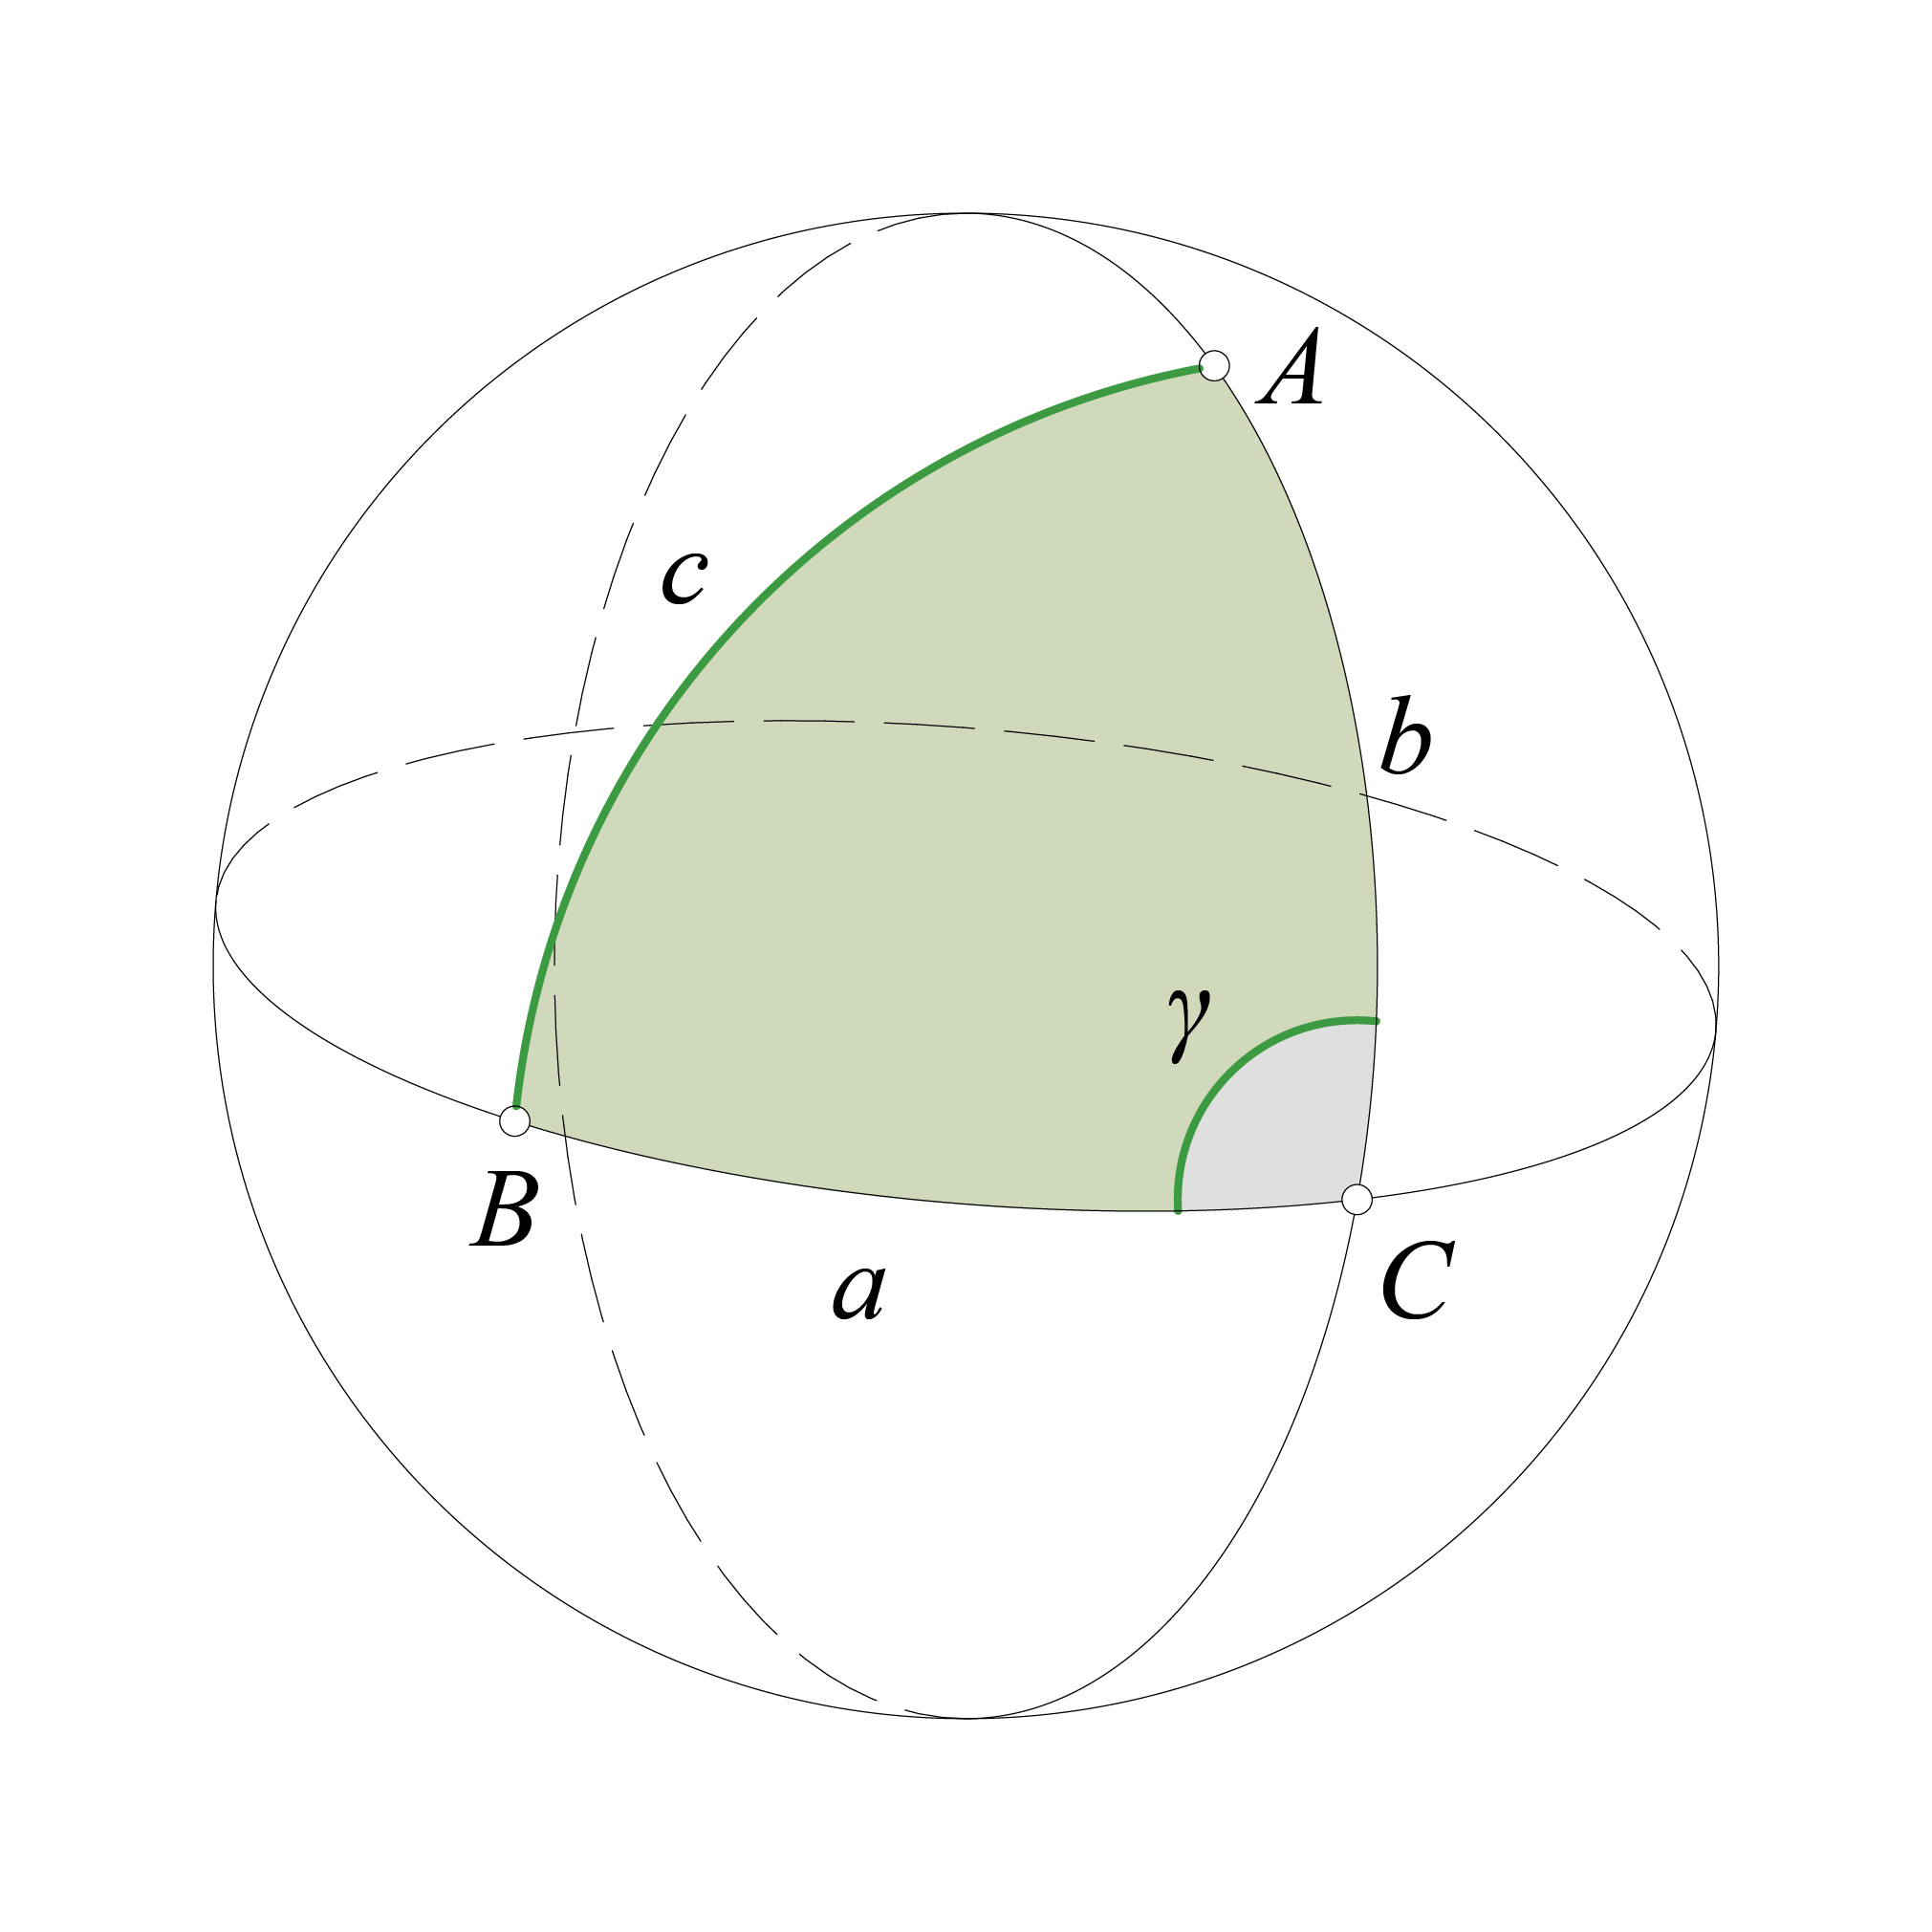
\includegraphics[width=0.4\textwidth]{kugel/Dualitaet.jpg}
    \captionof{figure}{Die Dualität auf der Kugel}
\end{center}

Nimmt man nun den Punkt $A$, welcher auf der Geraden $b$ liegt, so verläuft die Duale Gerade $a$ durch den zur Geraden $b$ dualen Punkt $B$. 
Aber nicht nur die Beziehungen zwischen Punkten und Längen bleiben erhalten. Auch die Winkel und Längen gehen ineinander über, wie im Beweis des Winkelkosinussatzes.
Der Winkel $\gamma$ zwischen den beiden Seiten $a$ und $b$ entspricht auf der Einheitskugel dem Abstand zwischen den zu der Geraden dualen Punkten $A$ und $B$.



\section{Navigation auf See}
Das besondere an Seekarten ist die inhaltliche Ausrichtung. Anders als die Landkarten muss sie Informationen enthalten, welche für den Kapitän und seine Besatzung von grosser Bedeutung sind. Vor allem in Küstennähe ist das navigieren eines Schiffes besonders gefährlich. So enthalten Seekarten Informationen über die Wassertiefen, Bodenbeschaffenheiten, Gezeiten, Küstenlinien, Landzungen und Windrichtungen.
Der Hauptunterschied dabei ist, dass auf der Landkarte feste Positionen definiert und aufgezeigt werden. Das einzige was sich bewegt, ist dabei der Reisende selbst. Bei der Seekarte ist das anders. Es werden veränderliche Einwirkungen der Natur festgehalten und die Schiffe auf See bewegen sich.

Dieser kleine Unterschied zeigt die Notwendigkeit auf, die Position und den Kurs seines Schiffes auf See immer ermitteln zu können.


\subsection{Geographische Koordinaten}
Bereits der griechische Astronom Claudius Ptolemäus verwendete in seiner Geographike Hyphegesis ein Gradnetz aus Längen- und Breitengraden. Der dabei verwendete Ferro-Meredian bildete bis ins 19. Jahrhundert den Null-Meredian auf der Erdkugel. 

XXX

Erst nach der Wiederentdeckung anfangs 15. Jahrhundert und der Übersetzung in die Lateinische Sprache, setzte sich die Geographike Hyphegesis, und damit das Ptolemäische Gradsystem durch.
Mit dem Vertrag von Tordesillas von 1494 gewann das Gradnetz an politischer Bedeutung und bürgerlichte sich ein.
Im Jahr 1884 wurde der Nullmeredian Ferro-Meredian durch den noch heute gültigen Greenwich Meredian, welcher in Grossbritannien seit 1738 in gebrauch war, ersetzt.

Zur geografischen Ortsbestimmung und damit der Festlegung seines eigenen Standortes auf einer Karte sind Längen- und Breitengrad nötig. 
Die Koordinaten werden traditionell im Sexagesimalsystem angegeben und setzen sich aus folgenden Komponenten zusammen:
\[
\begin{aligned}
&\text{Grad } (^{\circ})
&
&\text{\bigg \vert}
&
&\text{Bogenminuten } (`)
&
&\text{\bigg \vert}
&
&\text{Bogensekunden } (``)
\end{aligned}
\]

Die Erdoberfläche wurde in je 360 Breiten- und Längengrade eingeteilt. Die Breitengrade haben zueinander einen Abstand von 111.31 km, dies entspricht auch dem Abstand der Längengrade am Äquator, welcher mit Zunehmender Nähe zu den Polen abnimmt.
\[
\begin{aligned}
&1^{\circ}
&
&\text{\bigg \vert}
&
&4 \text{ Minuten}
&
&\text{\bigg \vert}
&
&111.31\text{ km}
\end{aligned}
\]

Eine ganze Erdumdrehung beinhalten $360 ^{\circ}$, was 1440 Minuten entspricht. Umgerechnet in Kilometer erhält man bei einer Umdrehung um den Äquator genau den Erdumfang von 40’071 km.

Eine ganze Erdumdrehung sind $360 ^{\circ}$ was 1440 Minuten entspricht, dabei erhält man genau den Erdumfang am Äquator: 40’074 km.
Nach einer vollen Umdrehung der Erde stellt sie sich wider in ihrer Ursprungsposition ein und ein neuer Tag beginnt. Dies zeigt, dass die Koordinaten in direktem Zusammenhang mit der Zeit stehen. Diese Erkenntnis wird später für die Navigation auf See von grosser Bedeutung sein.



\subsection{Erdachsenneigung}
Die Erdachse, auch Rotationsachse genannt, ist um ca. $23.5^{\circ}$ geneigt.
Daraus lassen sich Phänomene wie die vier Jahreszeiten oder die verschiedenen längen der Tage ableiten.
Für die nautische Navigation hat die Erdneigung eine grosse Bedeutung, da je nach Neigung andere Sterne zu beobachten sind. Auch ist die Sonne an einem anderen Ort am Himmel zu finden.

\begin{center}
        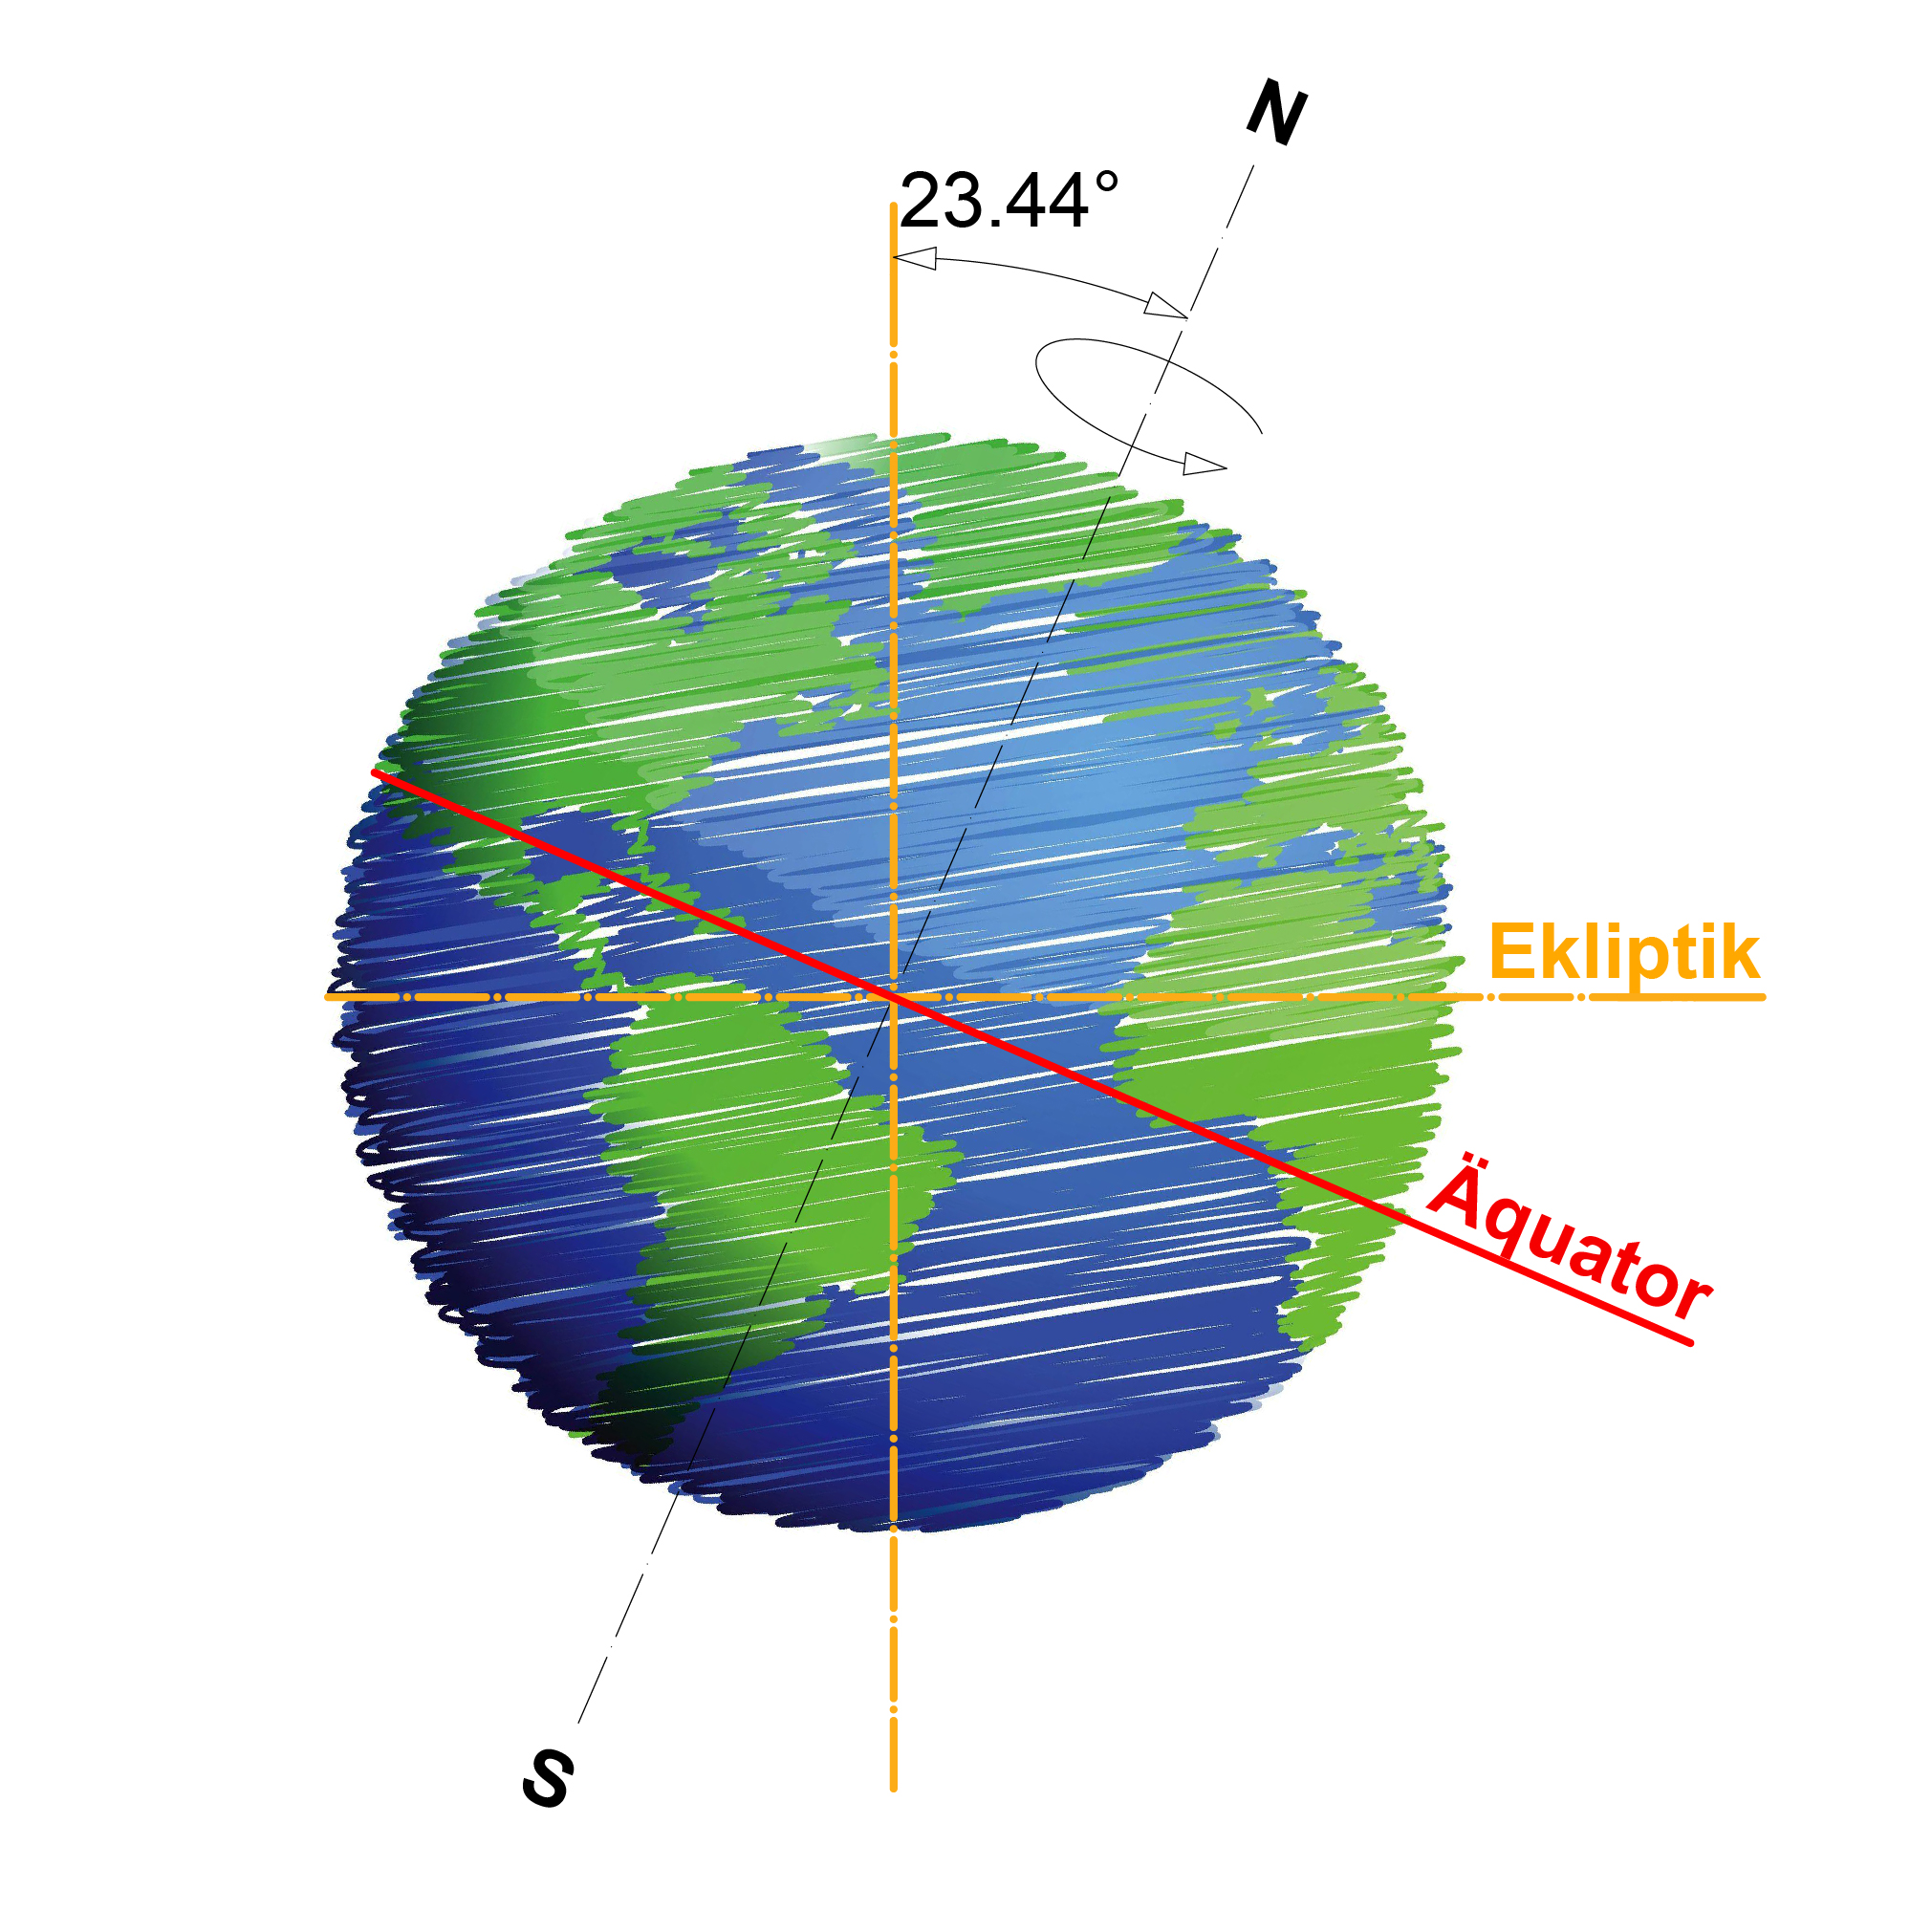
\includegraphics[width=0.4\textwidth]{kugel/Ekliptik.jpg}
    \captionof{figure}{Bild Erdneigung}
\end{center}

Der Schnittpunkt dieser beiden Kreise wird als Frühlings- bzw. Herbstpunkt bezeichnet und ist jeweils am 21. März bzw. 21. Oktober des Jahres.


\subsection{Zeitzonen der Erde} \label{Zeitzonen} 
Wenn man nun die verschiedenen Zeitzonen der Erde betrachtet, macht die Verschiebung von jeweils genau einer Stunde durchaus Sinn, es lässt sich auf die Längengrade schliessen.
Zwischen den verschiedenen Zeitzonen liegen 15 Längengrade:
\begin{align*}
\text{15 Längengrade à 4 Minuten = 60 Minuten Zeitverschiebung = ca. 1665 km}
\end{align*}

Dabei ist die Zeitzone, in welcher Mitte sich der Greenwich Meredian befindet, die \textit{Greenwich Mean Time (GMT)}, welche bis 1928 als Weltzeit galt. Im Jahr 1972 wurde diese umbenannt in die \textit{Coordinated Universal Time (UTC)} und wird von da an als Weltzeit und Startpunkt für die Aufteilung der Zeitzonen verwendet. Der Meridian blieb der selbe.


\section{Der Breitengrad}
Die Breitengrade bilden die bereits genannten Kleinkreise auf der Kugeloberfläche. Sie verlaufen in einem Abstand von etwa 111 km parallel zum Äquator. Der Äquator stellt gleichzeitig die Mitte zwischen Nord- und Südhalbkugel dar und teilt die Erdkugel in zwei gleich grosse Hälften. Somit bildet er einen natürlichen Nullpunkt für die Breitengrade.
Um zu wissen, auf welcher Halbkugel man sich befindet, spricht man von nördlicher und südlicher Breite. Für die Nordhalbkugel werden positive und für die Südhalbkugel negative Werte geschrieben. So ist auf den ersten Blick erkennbar auf welcher Halbkugel der Erde man sich befindet.

\begin{center}
        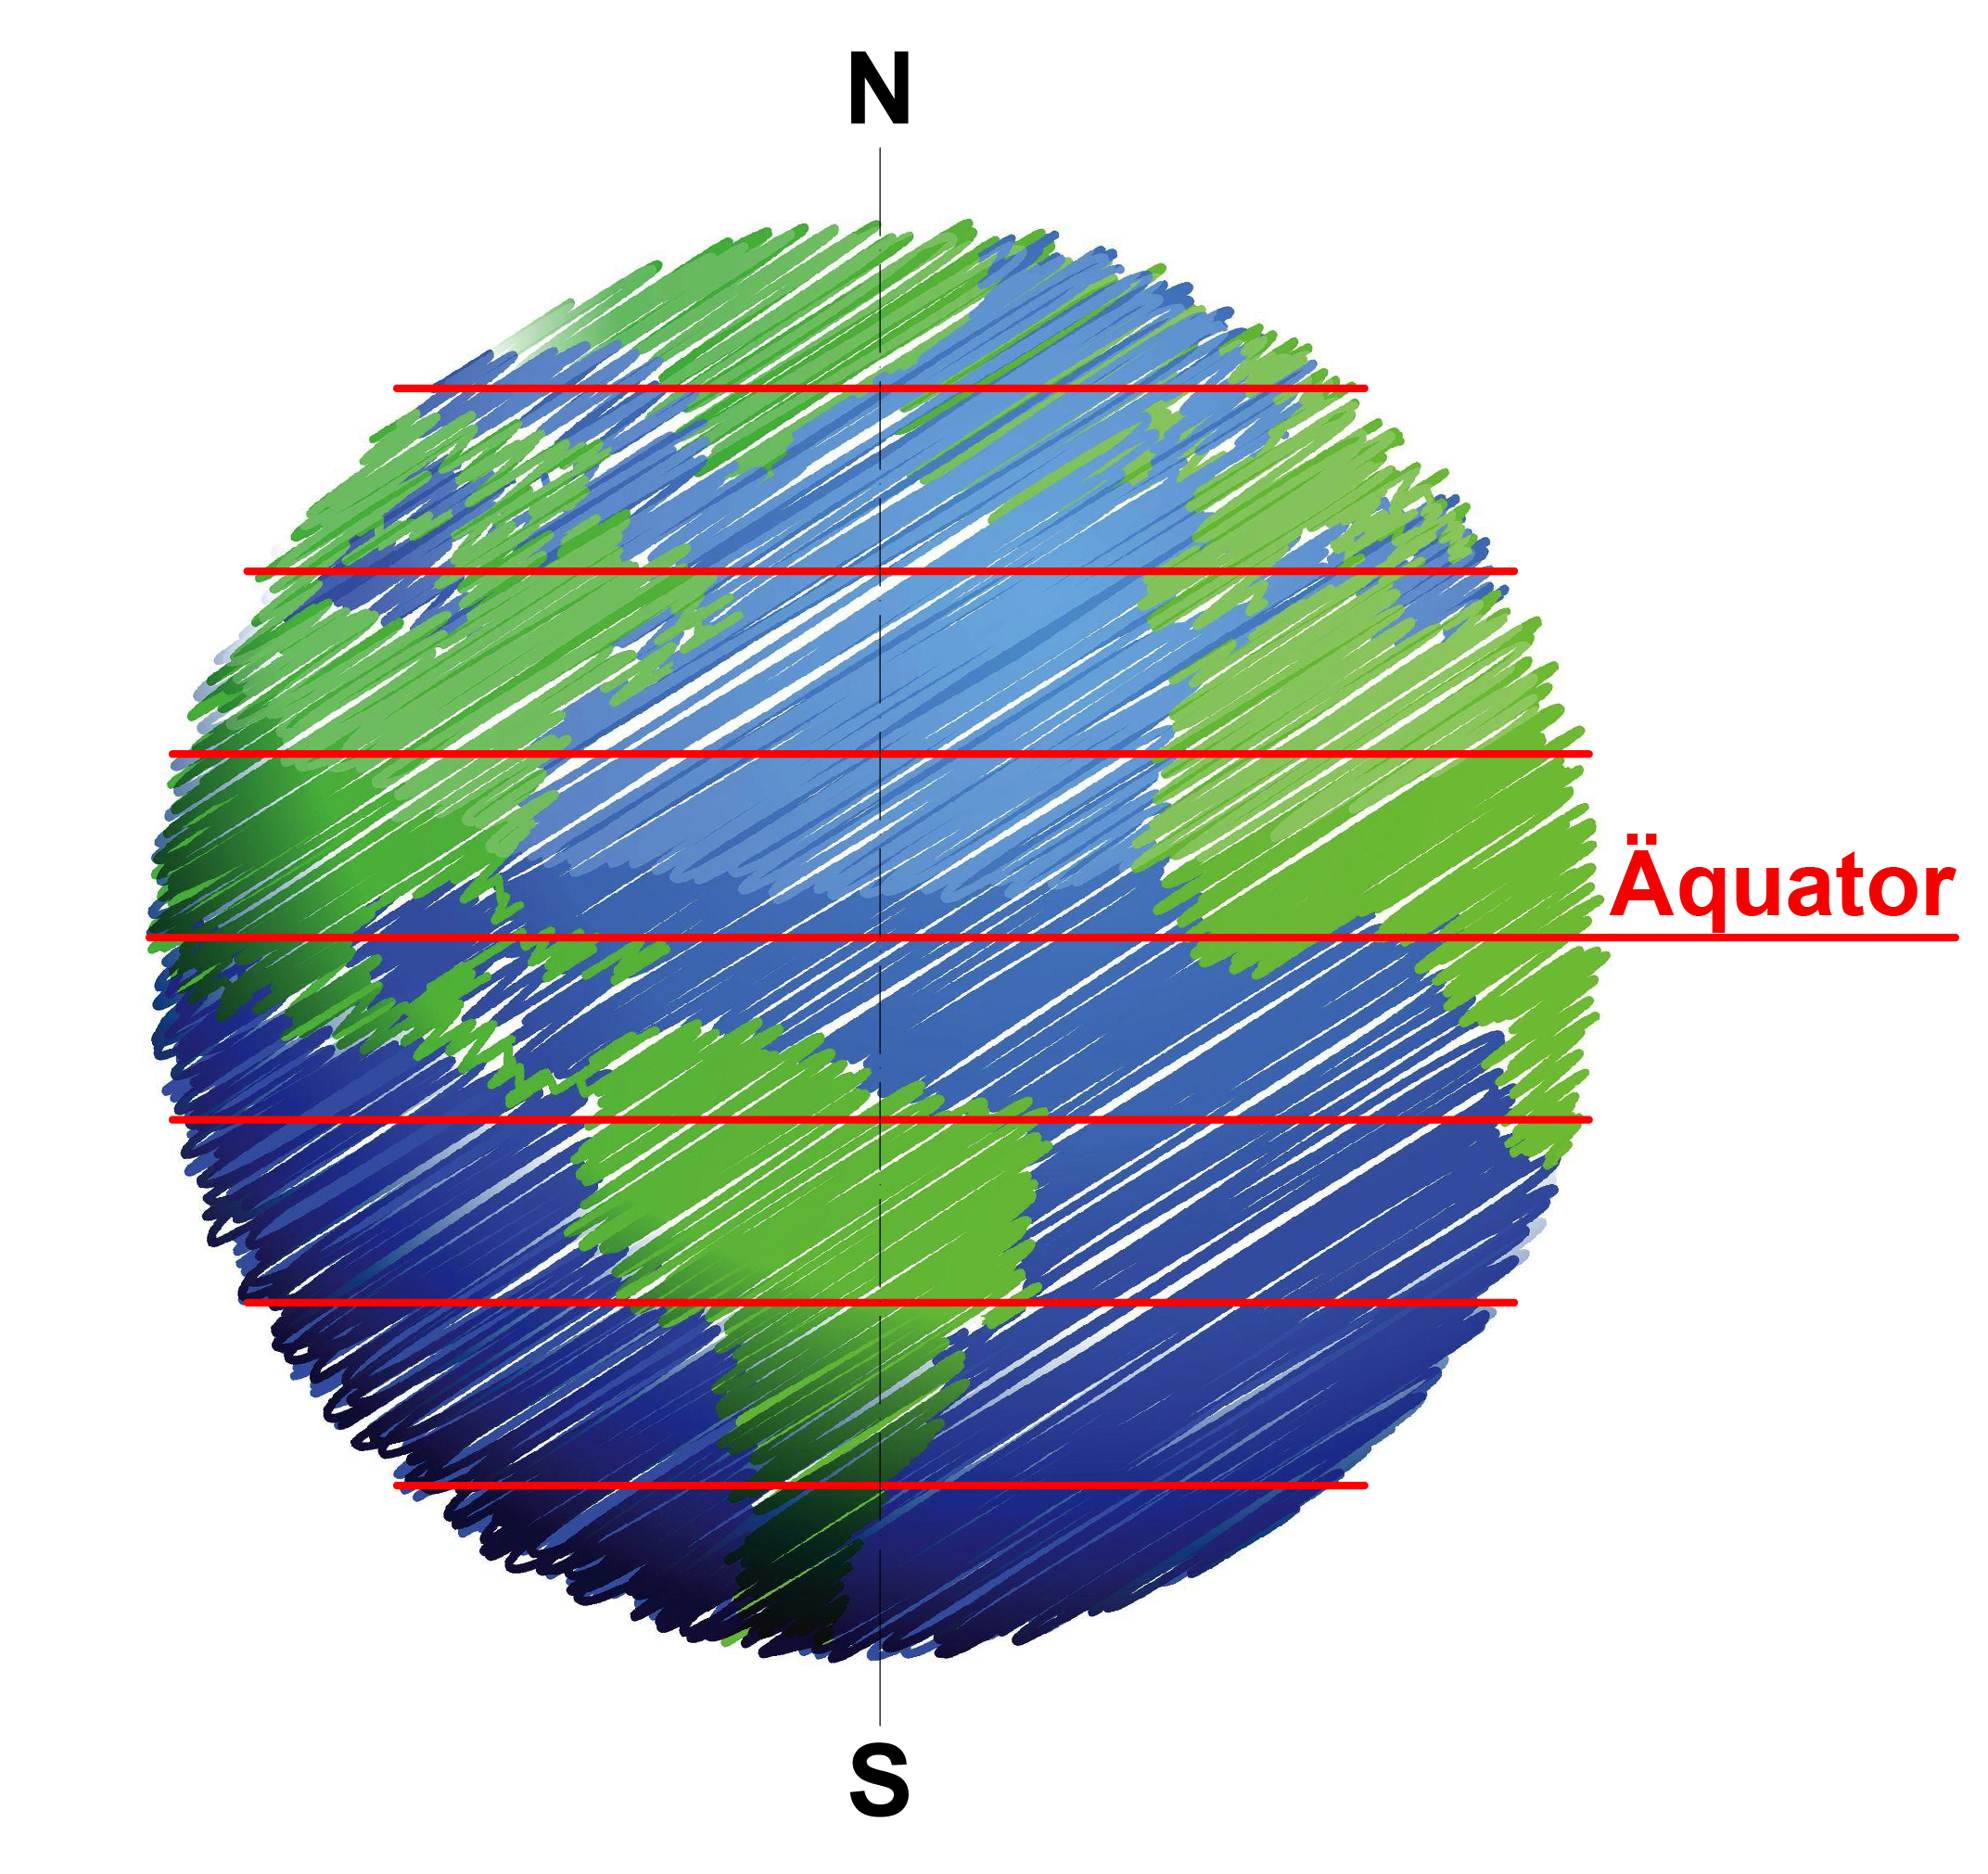
\includegraphics[width=0.4\textwidth]{kugel/BreiteErdkugel.jpg}
    \captionof{figure}{Breitengrade auf der Erde, mit dem Äquator als Nullpunkt}
\end{center}


\subsection{Geografische Breite $\phi$}
\begin{definition}
Die geografische Breite eines Standortes ist der Winkel am Erdmittelpunkt zwischen der Ebene des Äquators und der Geraden zum Standpunkt auf der Erdoberfläche.
\end{definition}

\begin{center}
        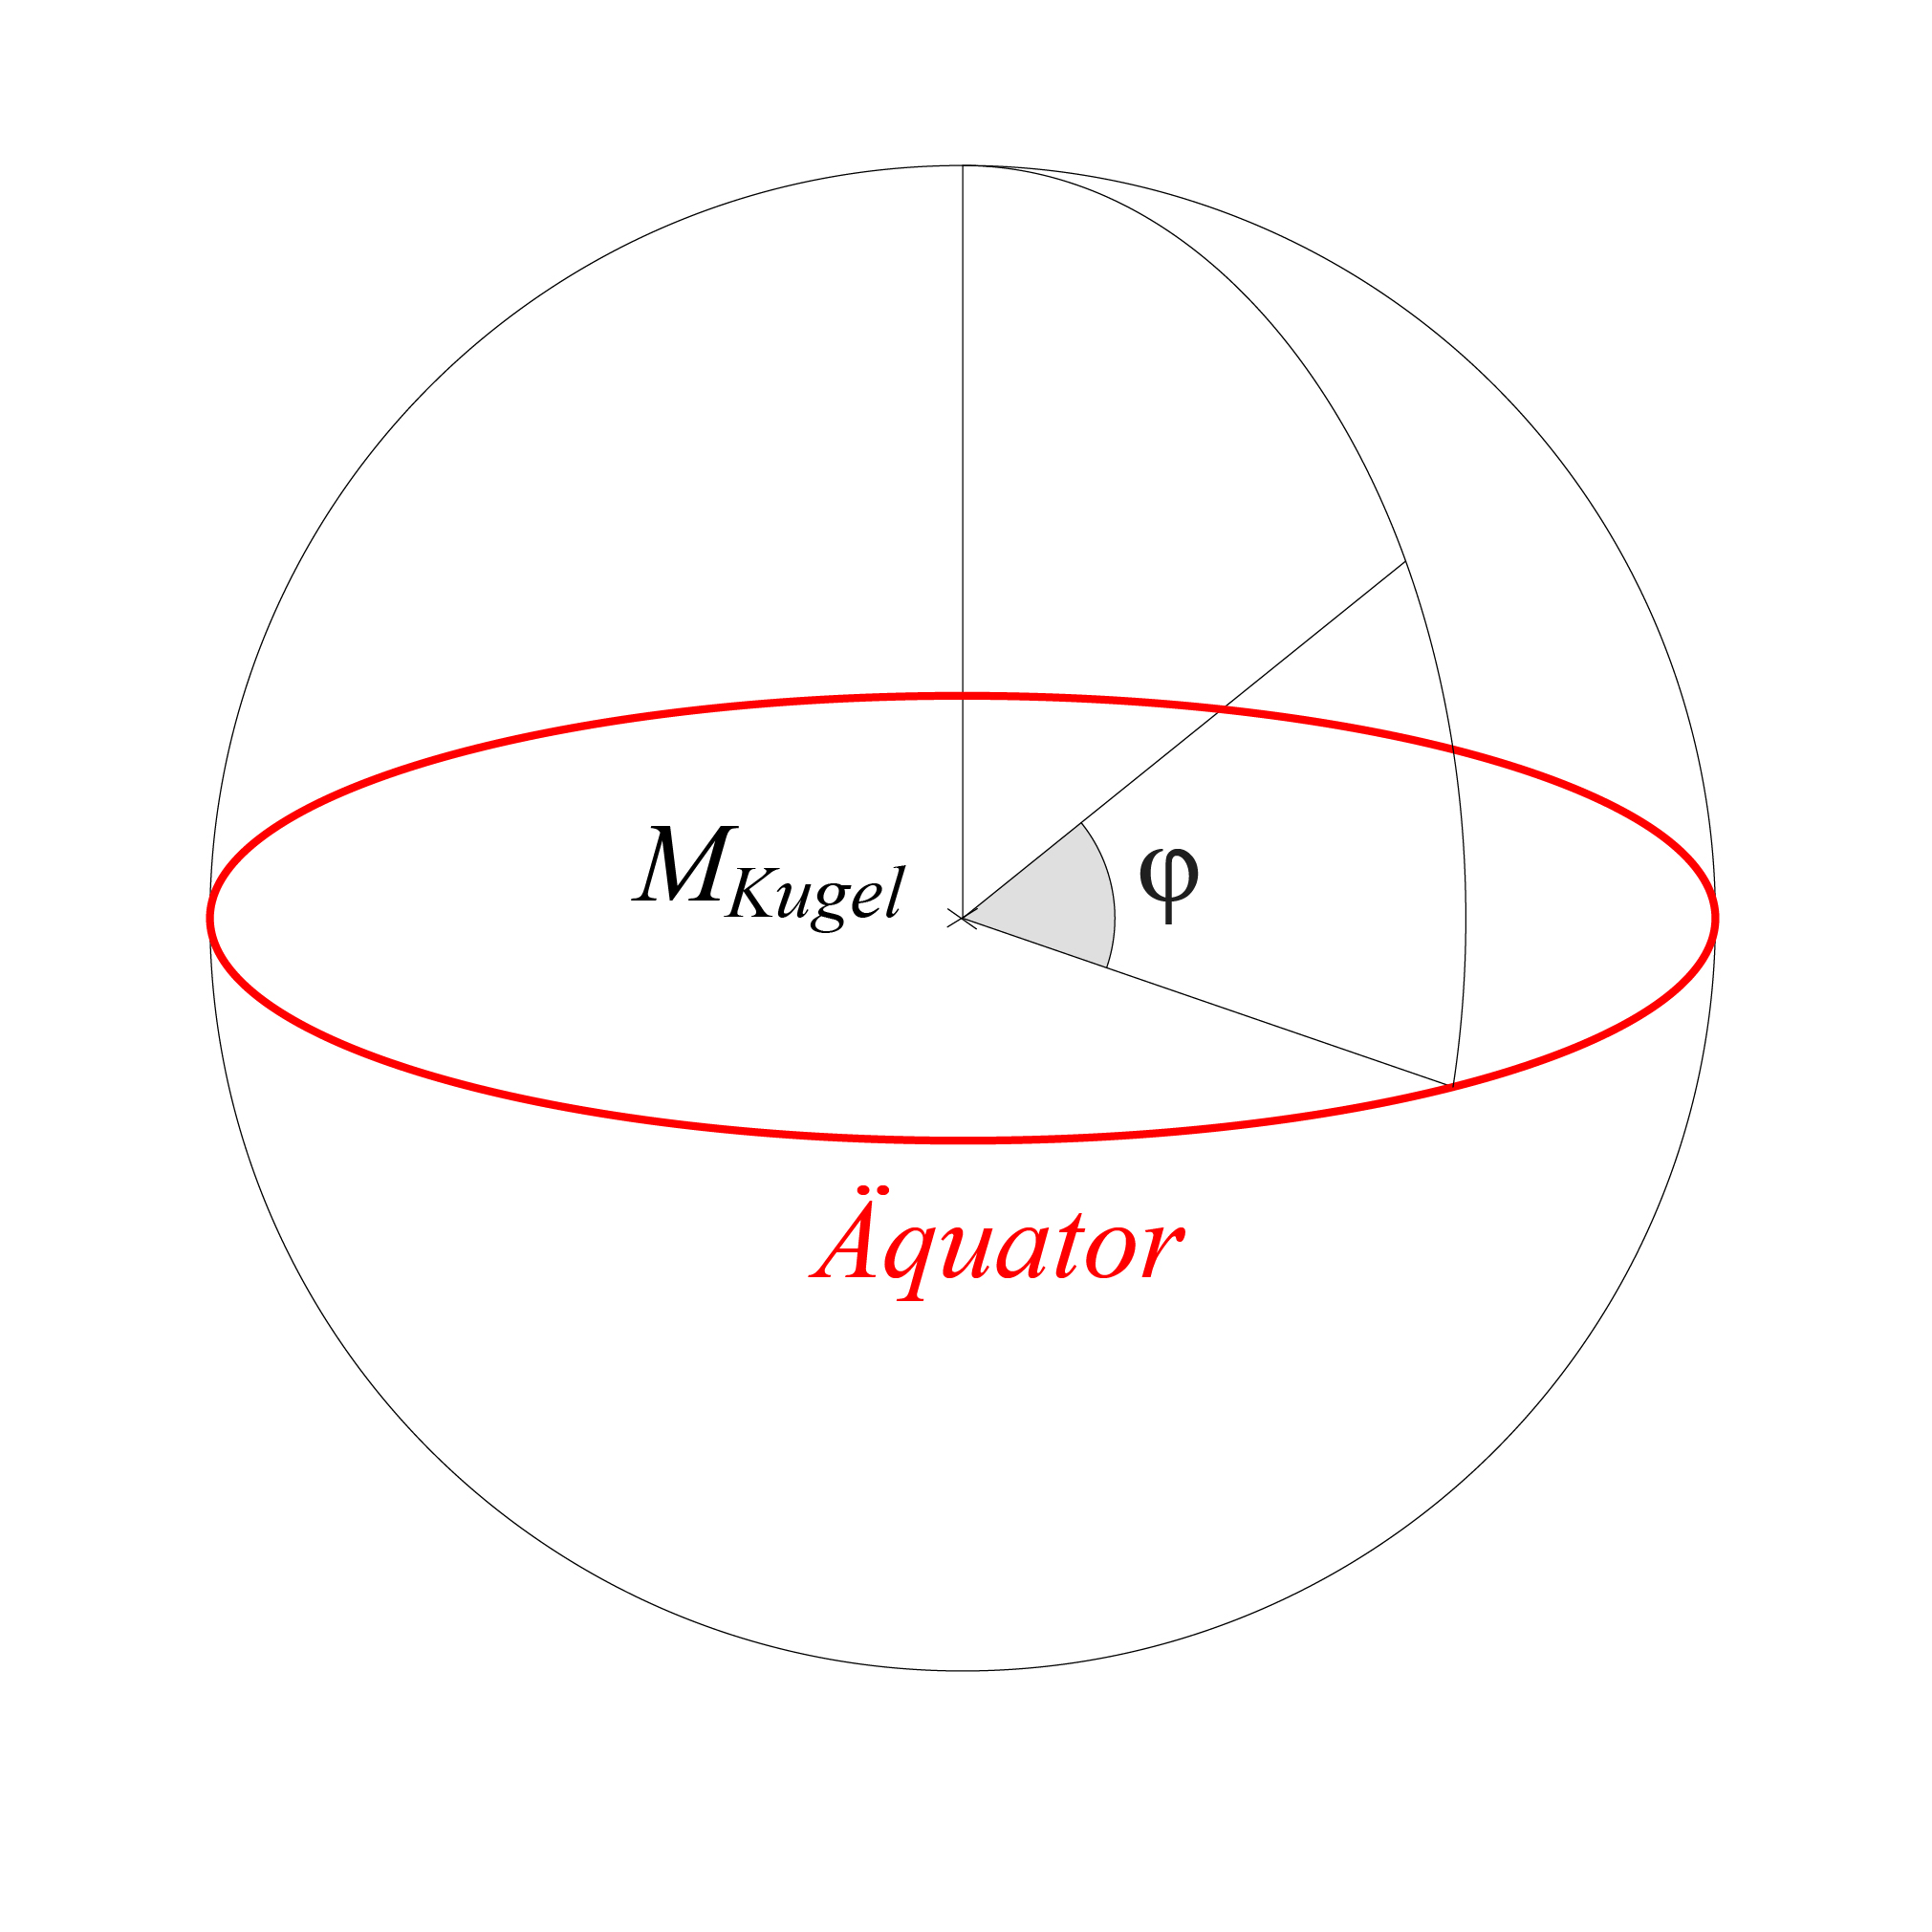
\includegraphics[width=0.4\textwidth]{kugel/GeografischeBreite.jpg}
    \captionof{figure}{Bild}
\end{center}


\subsection{Navigation mit den Breitengraden}  \label{BreitengradM}
Da der Breitengrad bereits sehr früh ziemlich präzise bestimmt werden konnte, nutzten bereits die Seefahrer um Christoph Kolumbus den Breitengrad zur Navigation ihrer Flotten.
Dieser lässt sich ziemlich einfach aus dem höchsten Sonnenstand oder einem Fixstern bestimmen. Dabei wird mit einem Jakobsstab\footnote{%
Der Jakobsstab ist ein früheres astronomisches Instrument zur Winkelmessung und wurde vor allem in der Seefahrt verwendet. Er ist in der Nautik der Vorläufer des Sextanten.} (später Sextant\footnote{%
Der Sextant ist ein nautisches Messinstrument zur Winkelmessung von Horizont und Fixstern (Gestirn)}) der Winkel zwischen dem Horizont und dem höchsten Sonnenstand oder einem Fixstern gemessen. Der Winkel, welchen man erhält, zieht man von 90° ab und erhält somit die geografische Breite. 

\begin{center}
        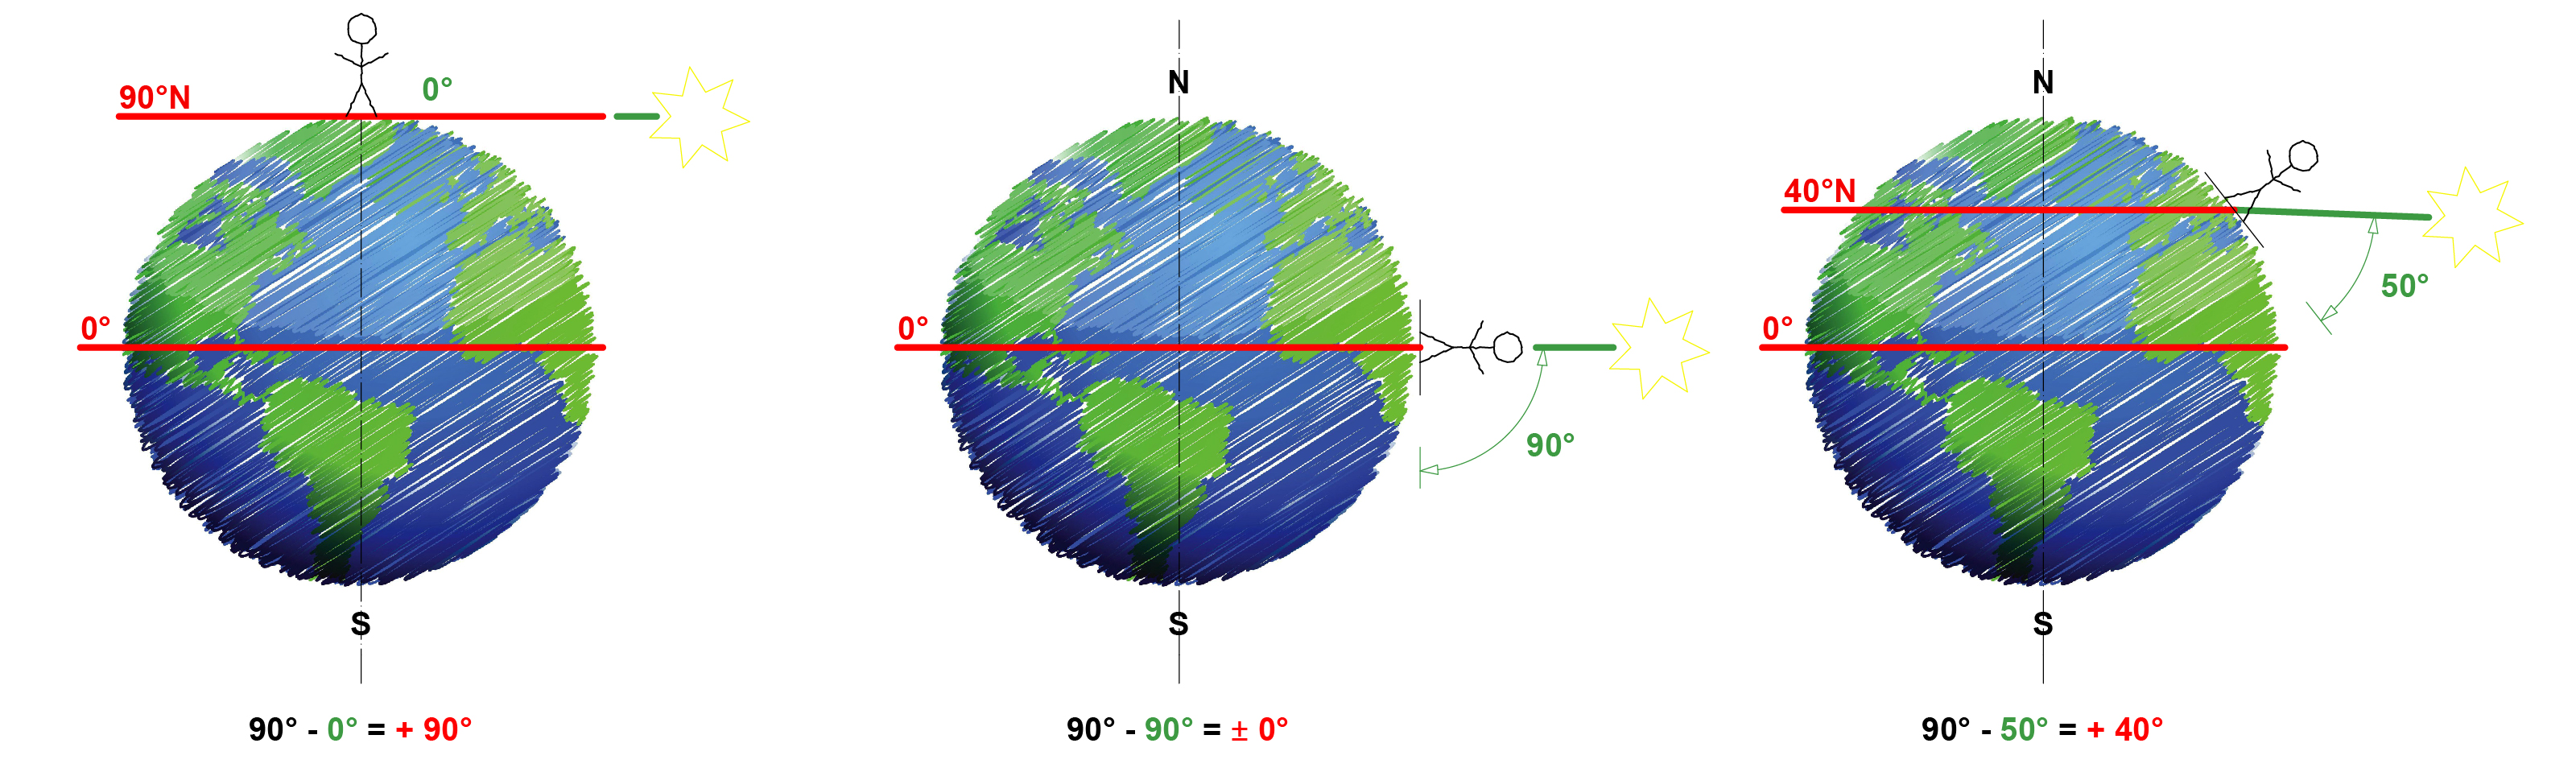
\includegraphics[width=0.9\textwidth]{kugel/Breitengrad.jpg}
    \captionof{figure}{Bild}
\end{center}

Wenn man sich auf der Nordhalbkugel befindet, ist der Polarstern ein sehr guter Fixstern. Befindet sich ein Schiff nun sehr nahe am Nordpol, steht dieser nahezu senkrecht am Himmels bei $90^{\circ}$. Würde es aber nahe dem Äquator stehen, erscheint dieser am Horizont bei $0^{\circ}$ und wäre je nach dem nicht mehr zu sehen.


\subsection{Korrekturbeiwert}
Da Breitengrade Kleinkreise sind, haben auch diese nicht immer den selben Radius. Daher segelt man am Äquator viel länger dem Breitengrad entlang um zum nächsten Längengrad zu kommen als in der nähe des Nord- oder Südpols.

\begin{center}
\renewcommand{\arraystretch}{1.5}
\begin{tabular}{ccc}
$1^{\circ}$ & 4 Minuten & 111.13km \\
$0.25^{\circ}$ & 1 Minute & 27.78km \\
$0.004166^{\circ}$ & 1 Sekunde & 463m 
\end{tabular}
\end{center}

Um die verminderte Strecke zu erhalten, müssen wir den Cosinus des gemessenen Breitengrades berechnen und diesen mit der Abweichung auf dem Äquator von 1 Sekunde multiplizieren.

\begin{center}
        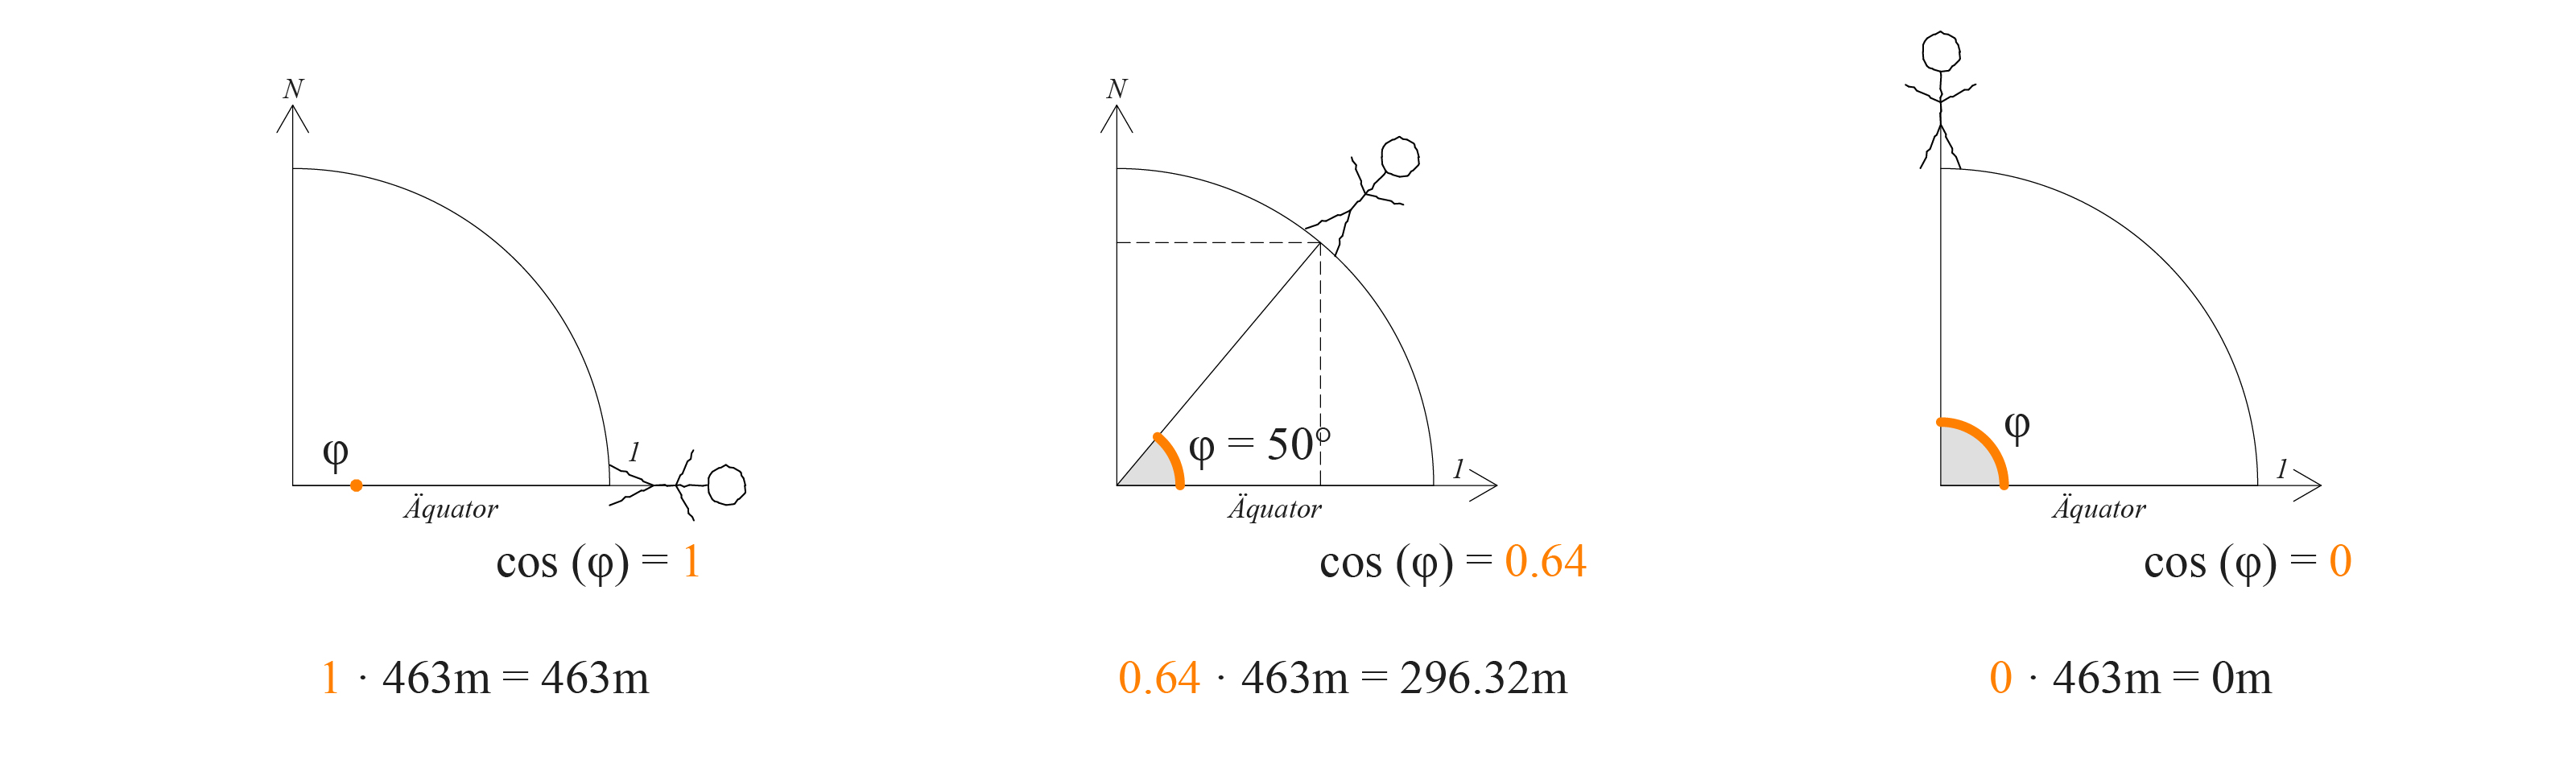
\includegraphics[width=0.9\textwidth]{kugel/Korrekturbeiwert.jpg}
    \captionof{figure}{Bild}
\end{center}

\[
\begin{aligned}
&\cos 90^\circ \cdot 463\text{m} = 463\text{m}
&
&\text{\bigg \vert}
&
&\cos 50^\circ \cdot 463\text{m} = 297.61\text{m}
&
&\text{\bigg \vert}
&
&\cos 0^\circ \cdot 463\text{m} = 0\text{m}
\end{aligned}
\]

Dies zeigt, je näher man den Polen ist, desto weniger weit muss man Segeln, um den nächsten Längengrad zu erreichen.



\section{Der Längengrad}
Die Längengrade bilden die bereits genannten Grosskreise auf der Kugeloberfläche.
Sie schneiden den Äquator im rechten Winkel und haben dort einen Abstand von etwa 111 km zueinander. Sie verbinden die beiden Pole, Nord und Süd, miteinander. Anders als bei der geografischen Breite ist in der Natur kein Längengrad gegeben, welcher den Nullpunkt darstellen könnte.

\begin{center}
        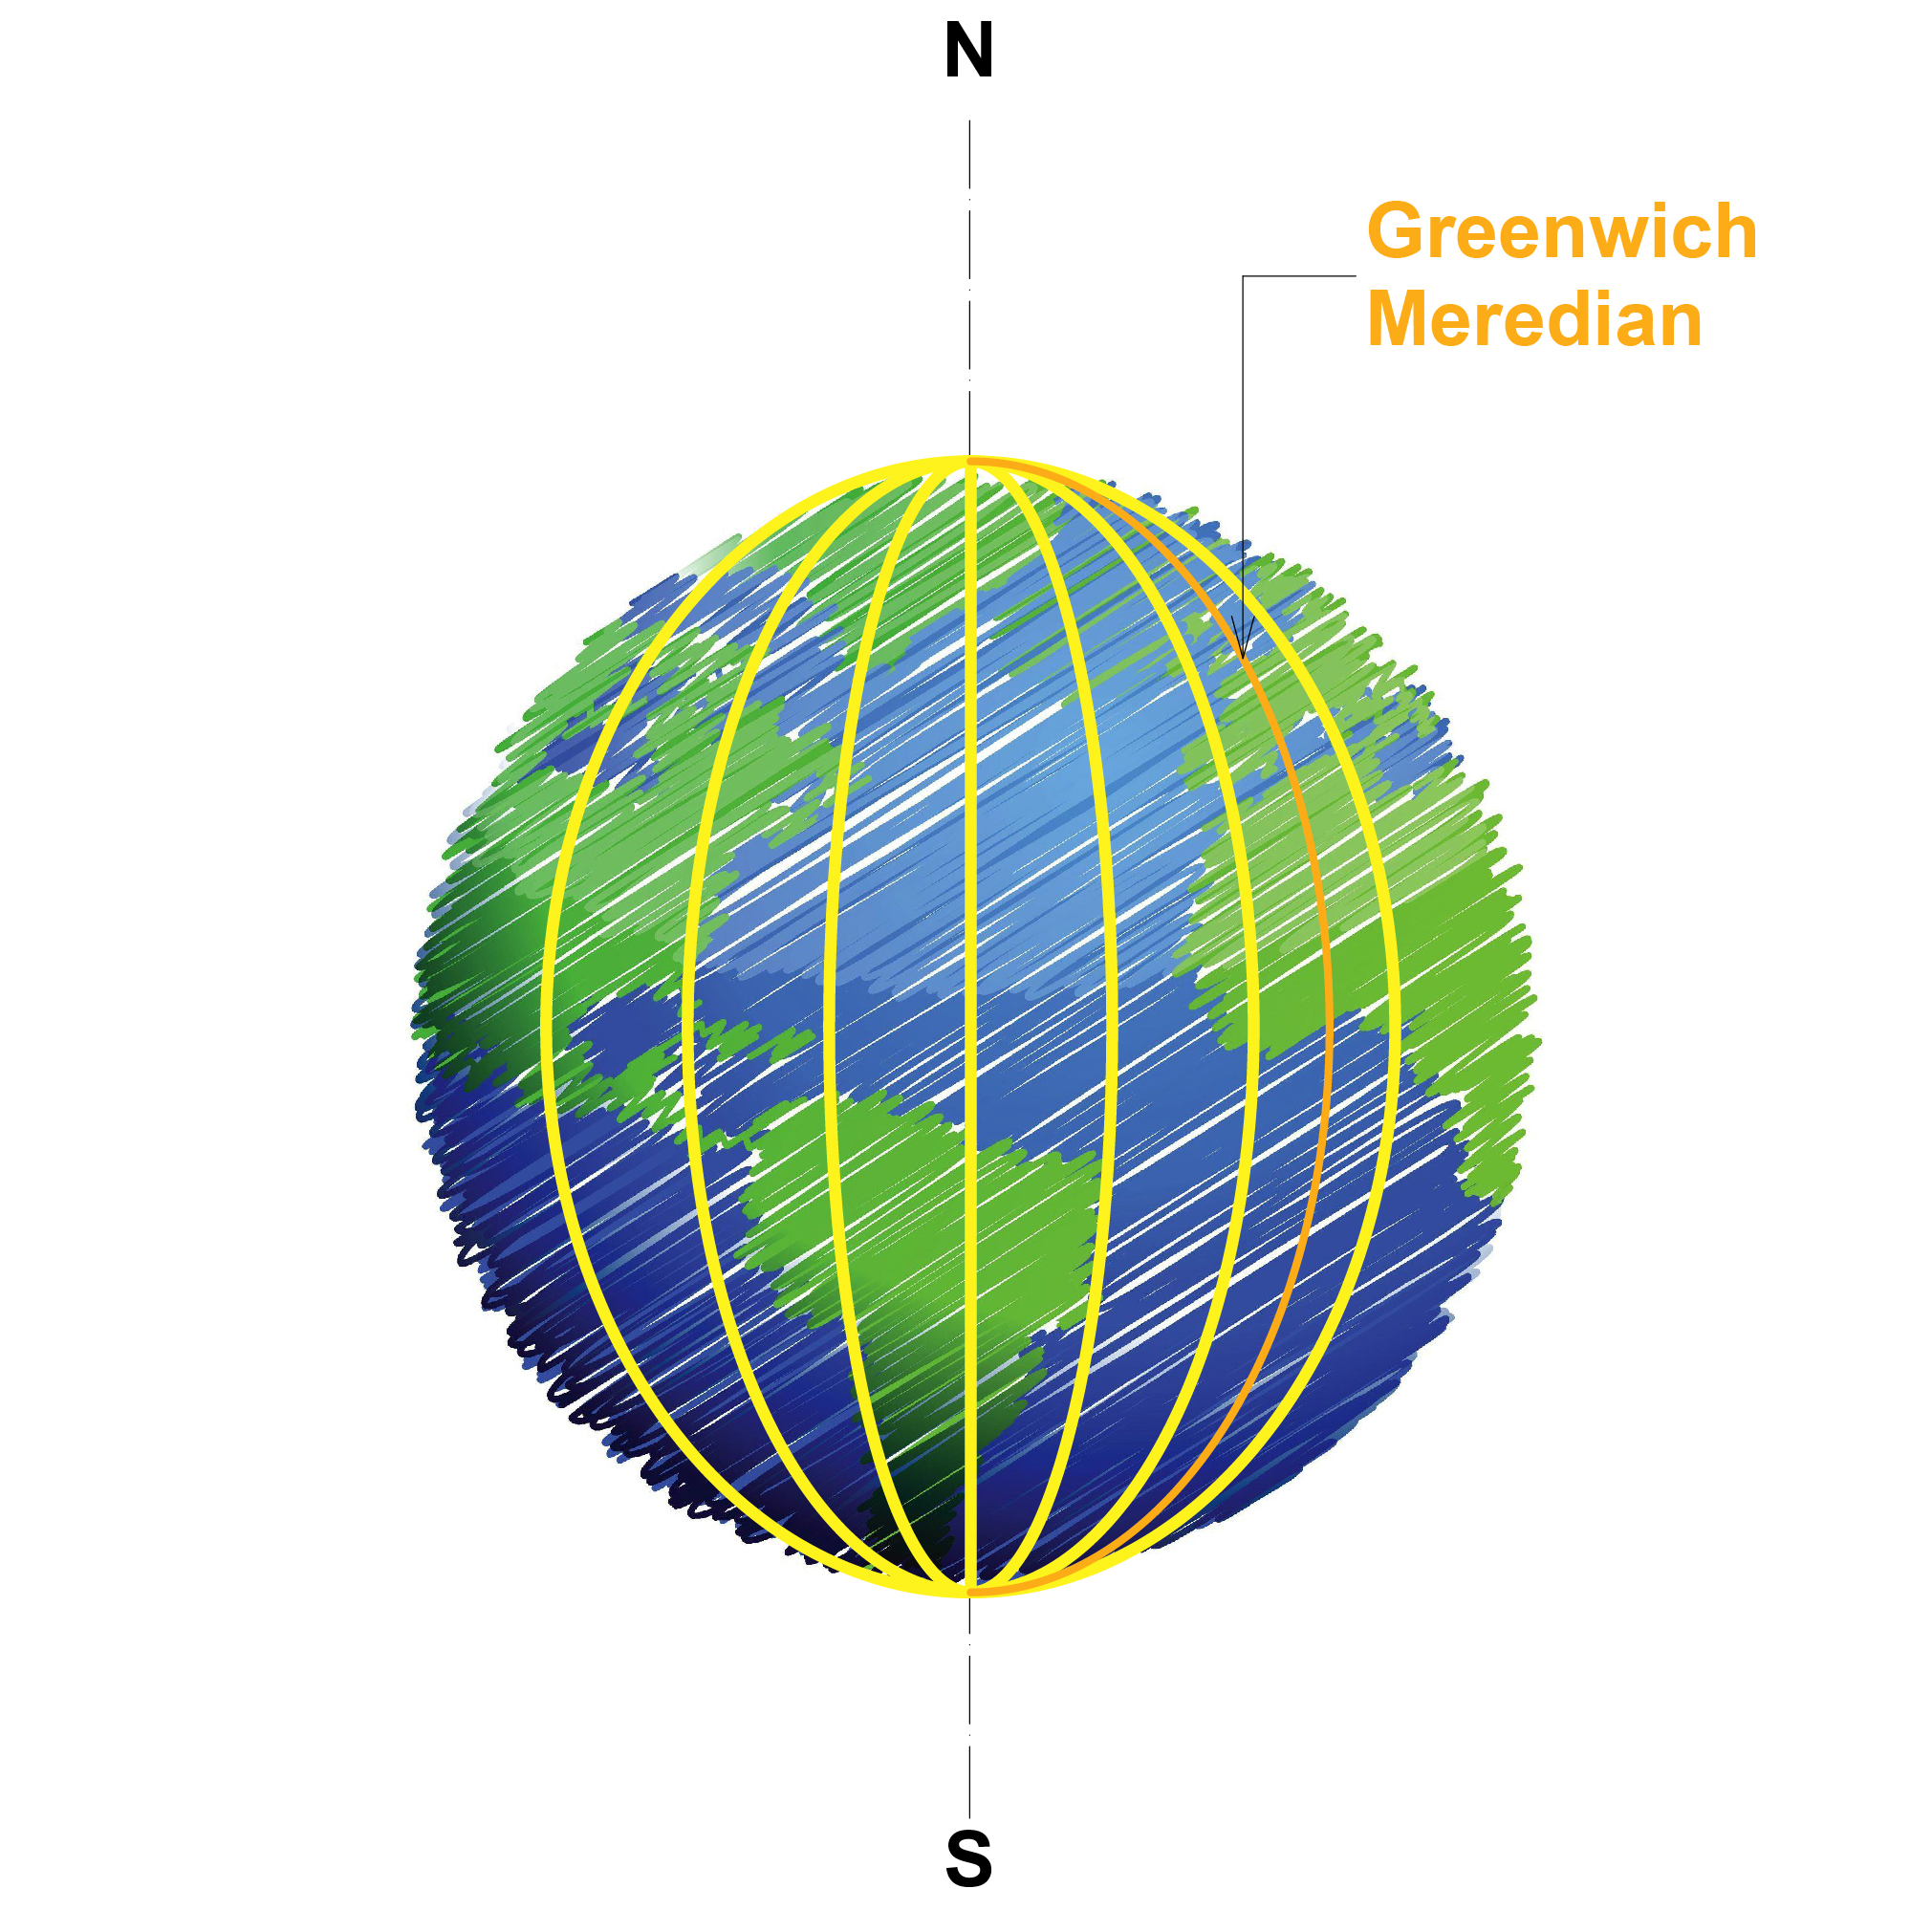
\includegraphics[width=0.4\textwidth]{kugel/Laengengrad.jpg}
    \captionof{figure}{Bild}
\end{center}


\subsection{Geografische Länge $\lambda$}
\begin{definition}
Die geografische Länge $\lambda$ ist der Winkel an der Erdachse zum Nullmeridian.
\end{definition}

\begin{center}
        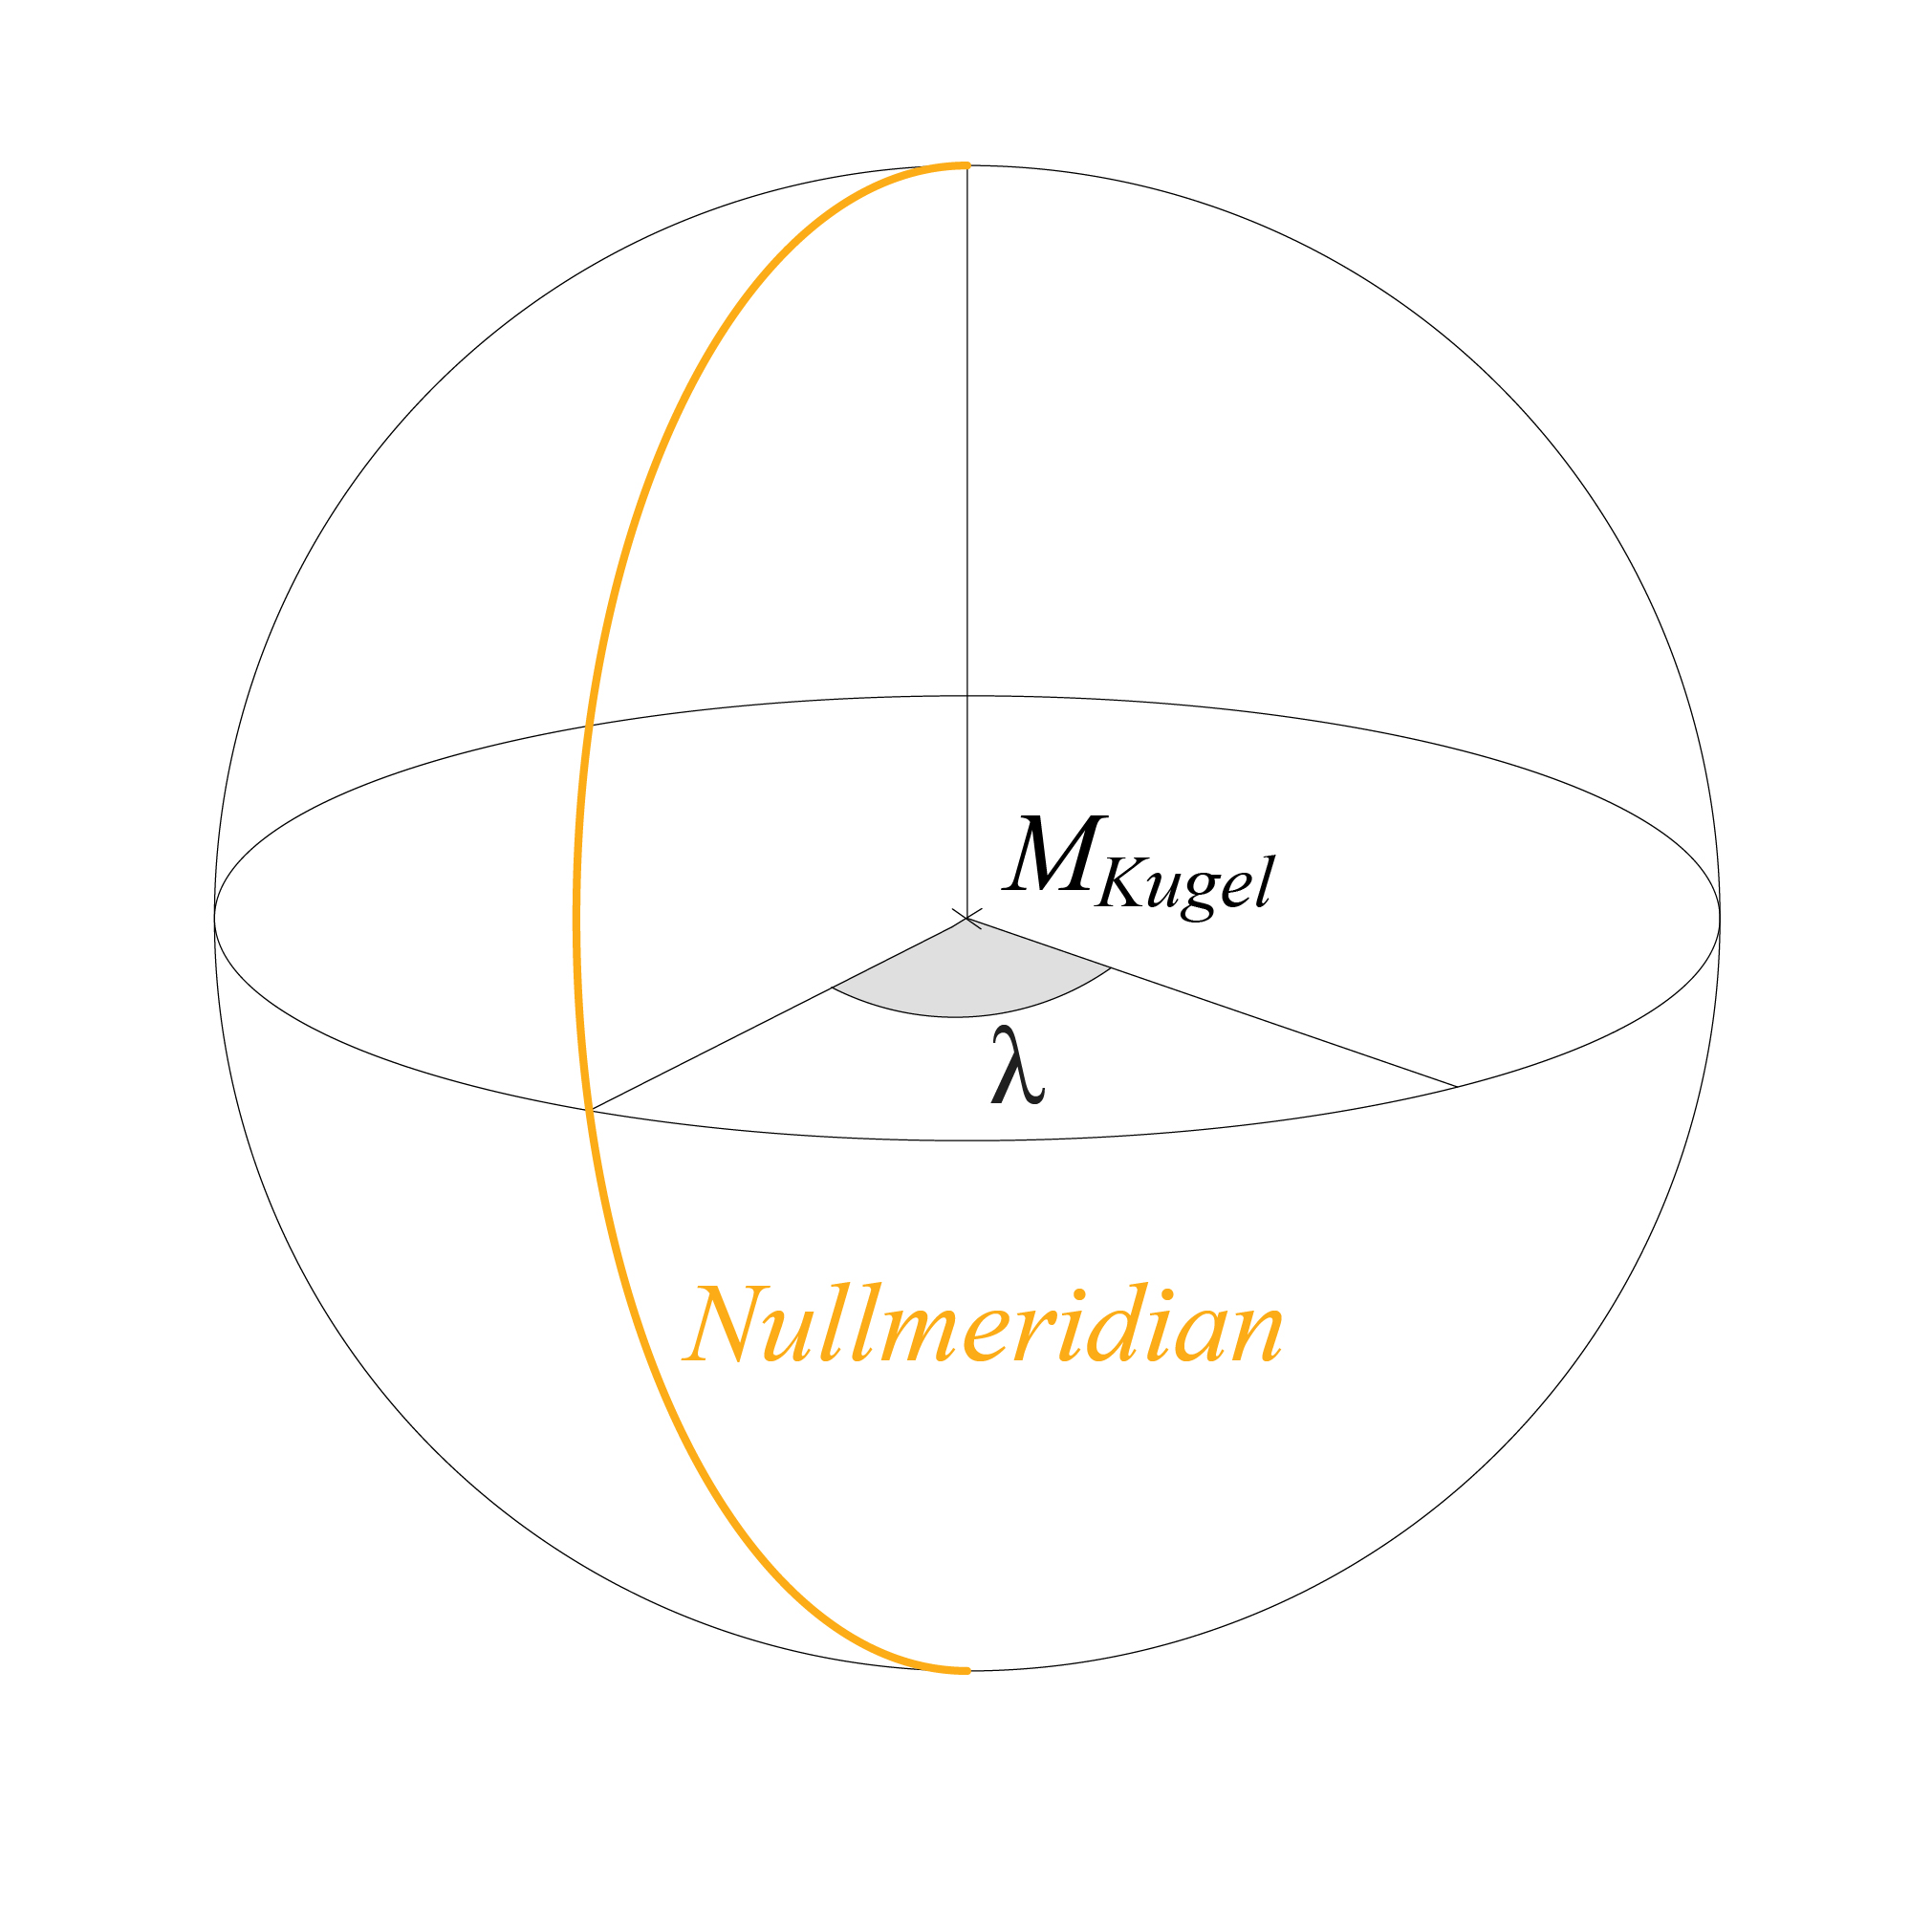
\includegraphics[width=0.4\textwidth]{kugel/GeografischeLaenge.jpg}
    \captionof{figure}{Bild}
\end{center}

\subsection{Navigation mit den Längengraden}
Die geografische Länge lässt sich nicht so einfach bestimmen die deren Breite.
Für die Berechnung auf See wird eine Referenzzeit eines Ortes mit bekannter Länge benötigt.
In der Zeit der Entdecker im 15. Jahrhundert, gab es noch keine mechanischen Uhren. Die Sonnenuhr war zudem ungeeignet, da diese nur die Tageszeit am Standort mass und nicht die am Referenzort selbst.

Die erste Pendeluhr wurde Mitte des 17. Jahrhunderts erfunden, was in der Schifffahrt aber auch nicht die Lösung brachte.

Pendeluhren auf einem Schiff sind ungeeignet, da das Pendel mit dem Wellengang aus dem Takt gebracht wird und somit die Uhr falsch geht.
Zu ungenau und gegen äussere Erschütterungen sehr empfindlich waren später die federgetriebene Uhren und die Unruh. Die verschiedenen Klimazonen, welche mit dem Schiff durchquert wurden, stellten ebenfalls ein grosses Problem dar. Das Metall zog sich fest zusammen oder dehnte sich aus, was dazu führte, dass die Uhr unregelmässig lief.



\section{The Board of Longitude — Das Längenproblem}
Das Längenproblem beschäftigte alle grossen Seefahrernationen Europas. Die fehlenden Längengrade bei der Navigation führten zu vielen Schiffsunglücken. Nicht selten kam es vor, das sich auf den untergegangenen Schiffen Schätze in der Höhe von halben britischen Staatshaushalten befanden. Der Verlust solcher Schiffe war enorm. Doch nicht nur die Navigation auf See war ein Problem, auch die Wirtschaft hatte darunter zu leiden. Die Schiffe mussten bis zur gewünschten geografischen Breite navigieren und segelten dann den Breitengrad entlang, um auch wirklich auf der gewünschten Position anzukommen. Dabei waren die Schiffe oft Wochenlang unterwegs und segelten die „Breiten ab“, um an die gewünschte Positionen zu kommen. Dies führte zu erheblichen Zeitverlusten und viel längeren Reisezeiten.

Bereits um 1600 hatte der König von Spanien ein Preisgeld ausgeschrieben für denjenigen, welcher eine Lösung für das Problem präsentieren konnte. Leider ohne Erfolg.

Nach einem tragischen Unglück im Jahr 1707, beidem der siegreiche Admiral Sir Cloudesley und seine 1’450 Mann sein Leben liessen, indem sie auf die Scilly-Inseln kurz vor Land’s End aufliefen und dabei die 21 Schiffe sanken, rückte das Problem wieder in den Vordergrund.
Sieben Jahre später und mithilfe einer Petition von William Whiston und Humphry Ditton, welche von Sir Isaac Newton und Edmond Halley unterstützt wurde, reagierte das britische Parlament.
Es schrieb folgende Preisgelder für eine praktische und brauchbare Lösung aus:
\[
\begin{aligned}
&\text{20’000£}
&
&\text{\big \vert}
&
&\text{Für eine Abweichung von max.} \frac{1}{2}^{\circ} \text{(etwa 55.5 km am Äquator)}
\\
\\
&\text{15’000£}
&
&\text{\big \vert}
&
&\text{Für eine Abweichung von max.} \frac{2}{3}^{\circ} \text{(etwa 74 km am Äquator)}
\\
\\
&\text{10’000£}
&
&\text{\big \vert}
&
&\text{Für eine Abweichung von max.} 1 ^{\circ} \text{(etwa 111 km am Äquator)}
\end{aligned}
\]
Eine Abweichung von 111km am Äquator entspricht 60 Seemeilen.
Auf der Höhe des Ärmelkanals und damit in der Nähe von London entspricht die Abweichung von $1 ^{\circ}$ noch 74 km.
Das Preisgeld entsprach einer enorm hohen Summe für die damalige Zeit. Der Kaufpreis für ein mittleres Schiff, welches zur See fahren konnte, lag bei etwa 1’500-2’500£. Ein einzelner Arbeiter lebte von 10£ im Jahr.

Würde man dieses Problem in der heutigen Zeit, mit einer maximalen Abweichung von einem halben Grad lösen, erhielte man 2’840’000£. Dies entspricht etwa einem Wert von 3’600’000 Schweizer Franken, je nach Wechselkurs.
Damit die Lösungsvorschläge kontrolliert und verwaltet werden konnten, wurde die Board of Longitude (Längenkommission) gegründet. Ihr gehörten die bedeutendsten Astronomen und Mathematiker dieser Zeit an, aber auch berühmte Persönlichkeiten aus Grossbritannien wie der Präsident der Royal Society und damit niemand anderen als Sir Issac Newton.



\subsection{John Harrison}
Harrison brachte sich das Handwerk des Uhrmachers selbst bei. Im Jahr 1713 und im Alter von 20 Jahren konstruierte er seine erste Pendeluhr. Später folgten weitere Pendeluhren und Standuhren. Durch seine Erfindungen der Grasshopper-Hemmung und des Rostpendels erreichten seine Uhren eine aussergewöhnliche Genauigkeit für die damalige Zeit. Die Abweichung pro Monat betrug dabei nur etwa eine Sekunde.
Erst 13 Jahre nach der Ausschreibung für die Lösung des Längenproblems tüftelte er an einer Konstruktion für eine Schiffsuhr und setzte sich mit dem Längenproblem auseinander.
Namhafte Astronomen in ganz Europa suchten nach astronomischen Lösungen für das Problem. Harrison jedoch setzte auf genaue Uhren und war somit unabhängig davon, ob man den Mond sah oder nicht.
1728 folgte sein erstes Konzept für eine schiffstaugliche Uhr. 1735 präsentierte er sein erstes Modell, die H1. Die Testfahrt mit der H1 an Bord von London nach Lissabon und zurück hielt die vorgeschriebene Genauigkeit ein und übertraf diese sogar. Die Reisedauer hatte jedoch nicht den vorgeschriebenen Bedingungen entsprochen.
\begin{center}
        \includegraphics[width=0.3\textwidth]{kugel/JohnHarrison.jpg}
    \captionof{figure}{Portrait von John Harrison mit der H4 - gemalt von P.K, Tassaert}
\end{center}
Das Hauptproblem war jedoch, dass Harrison als nichtstudierter Laie einem gelehrten Gremium dem Board of Longitude gegenüber stand. Dies verzögerte seine Annahme um Jahrzehnte. Der Krieg verlief ebenso zu Ungunsten Harrisons, denn seine weiteren Uhren, die H2 und H3, wurden nie getestet. Das Britische Empire wollte verhindern, dass die Uhren in die Hände der zur dieser Zeit verfeindeten Spanier gelangten.

Mit einem Durchmesser von 13cm und 1.45kg folgte im Jahr 1753 endlich der Durchbruch.
Die Taschenuhr H4 stellte alle anderen Uhren in den Schatten. Auf einer 81-tägigen Fahrt nach Jamaika zeigte sie eine Abweichung von nur 5 Sekunden.
Das Gremium entschied erneut gegen Harrison und beauftragte ihn seine Uhr vor ihren Augen zu zerlegen, zu erklären und Konstruktionszeichnungen anzufertigen.
Harrison erhielt vom britischen Parlament ein Preisgled von 10’000£, um eine Kopie seiner Uhr H4 anzufertigen. Er musste beweisen, dass seine Uhr nicht nur zufällig so genau lief.

\begin{figure}[!htb]
\centering
    \subfigure[H1 - 1735]{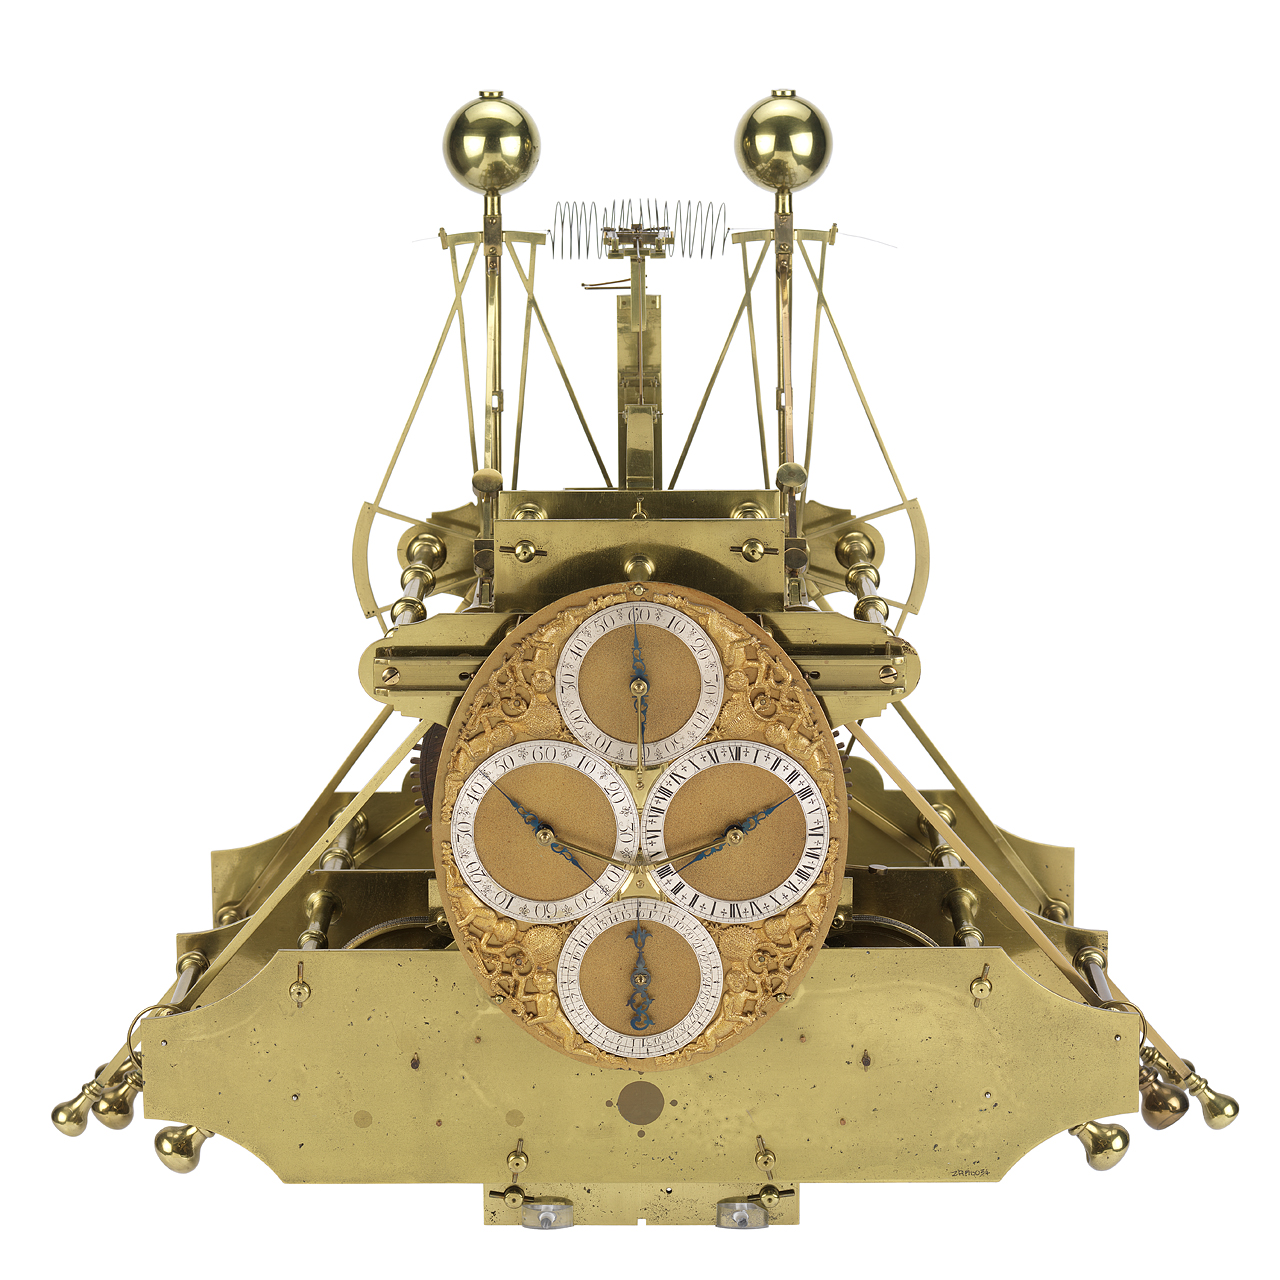
\includegraphics[width=0.25\textwidth]{kugel/H1.jpg}} 
\quad \quad
\centering
    \subfigure[H2 - 1737]{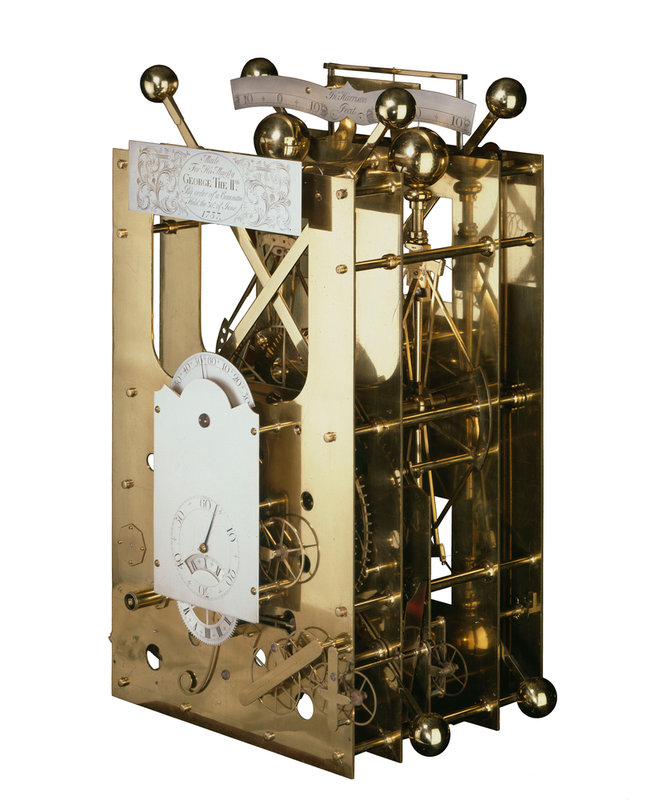
\includegraphics[width=0.25\textwidth]{kugel/H2.jpg}} 
\quad \quad
\centering
    \subfigure[H4 - 1753]{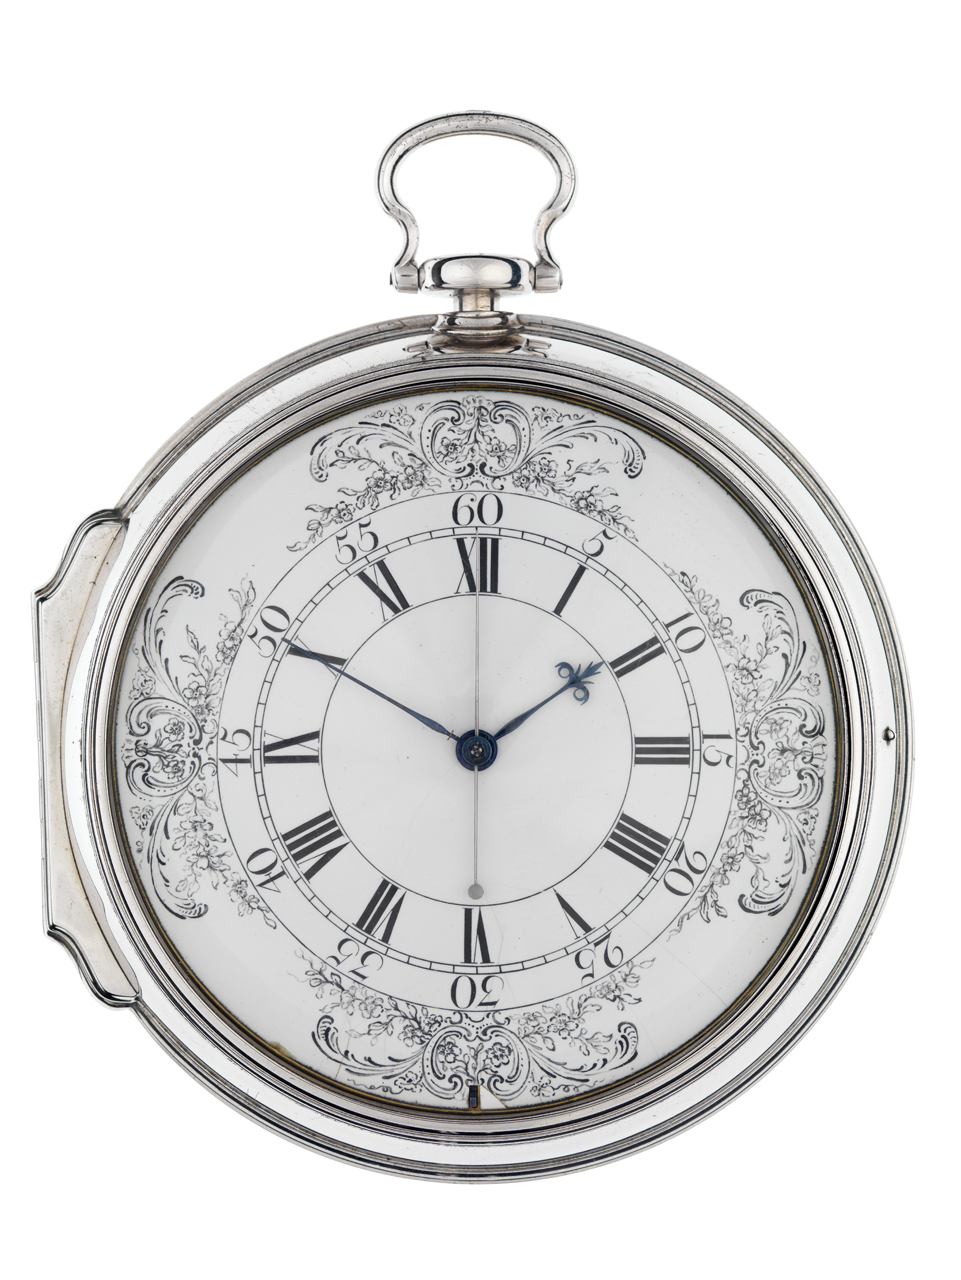
\includegraphics[width=0.25\textwidth]{kugel/H4.jpg}} 
\caption{Harrisons Uhren im Laufe der Zeit} 
\end{figure}
Der bekannte Londoner Uhrmacher Larcum Kendall fertigte danach eine Kopie der H4 an und zeigte somit, dass die Uhr den Anforderungen entsprach.

Das Geld blieb für Harrison aber weiterhin aus. Erst nachdem der britische König Georg III dem Parlament angedroht hatte, persönlich zu erscheinen und Harrison das Geld zuzusprechen, schrieben diese ihm 3 Jahre vor seinem Ableben weitere 8750£ zu.

8 Monate vor seinem Tod und der Rückkehr der K1 (Kopie der H4) ging die Vision Harrisons in Erfüllung. Es war nun definitiv bewiesen, dass seine Uhr auf dem offenen Meer zur Bestimmung des Längengrades taugte. James Cook, der berühmte britische Seefahrer und Entdecker, welcher die Uhr K1 auf See mitnehmen und testen durfte, nannte die Uhr liebevoll seinen \textit{nie versagenden Führer}.
Auf der Grundlage Harrisons Uhr H4 wurden die Schiffschronometer noch lange Zeit gebaut.



\subsection{Tobias Mayer}
Etwa zur gleichen Zeit wie John Harrison entwickelte Tobias Mayer\footnote{%
Tobias Mayer (1723-1762) studierte nie an einer Universität und war trotzdem ein annerkannter Wissenschaftler seiner Zeit in den Bereichen Astronomie, Geo- und Kartografie, Mathematik und Physik.}
ebenso eine Lösung für das Längenproblem.
\begin{center}
        \includegraphics[width=0.2\textwidth]{kugel/TobiasMayer.jpg}
    \captionof{figure}{Portrait von Tobias Mayer - Kupferstich von Conrad Westermayr}
\end{center}
Seine Mondkarten galten ein halbes Jahrhundertlang als unübertroffen. Der Ruhm galt aber hauptsächlich seinen Mondkarten, welche er im Jahr 1755 in einer erweiterten Version dem britischen Parlament vorlegte.
Mit ihnen konnte man die Geografische Länge bis auf 5 Bogensekunden genau bestimmen. Dies entsprach am Äquator $0.5 ^{\circ}$, was wiederum eine Genauigkeit von 55.565km entsprach.

Eine Lösung für das Längenproblem war gefunden. Die Publikation seiner Mondtafeln fand 1767 unter dem Titel \textit{Theoria lunae juxta systema Newtonianum} in London statt, 5 Jahre nach Mayers Tod. 
Seine Witwe schickte die publizierten Mondkarten über die Universität Göttingen nach Grossbritannien. Sie erhielt von der britischen Regierung eine Prämie in der Höhe von £ 3’000.-.

Im Jahr 1935 wurde ein Krater auf der westlichen Mondvorderseite nach dem deutschen Astronomen benannt. Er trägt fortan den Namen T.Mayer.
\begin{center}
        \includegraphics[width=0.3\textwidth]{kugel/Mondkarte.jpg}
    \captionof{figure}{Thomas Mayers Mondkarte}
\end{center}


\section{Nautisches Dreieck (Astronomisches Dreieck)}
Um seine Koordinaten bestimmen zu können, genauer gesagt um den Längengrad zu ermitteln, ohne moderne GPS-Geräte, ziehen wir ein altbewährtes Hilfsmittel aus der Seefahrt zur Hilfe - Das Nautische Dreieck.

Es dient zur Positionsbestimmung auf dem offenen Meer oder anderen Gebieten, in denen keine Orientierungspunkte wie Landzungen oder Gebirgsketten zu Hilfe genommen werden können.

Das Nautische Dreieck an der Himmelskugel hat folgende Eckpunkte:
\begin{itemize}
\item Himmelsnordpol ($N$) - auch bekannt als Polarstern
\item Gestirn ($S$) - ein uns bekannter Stern, wir verwenden im Beispiel die Sonne
\item Zenit ($Z$) - der Himmelspunkt, welcher sich senkrecht über uns befindet
\end{itemize}

Dieses Kugeldreieck wird das nautisches Dreieck genannt.

%SKIZZE NAUTISCHES DREIECK

\subsection{Berechnung der Dreiecksseiten}
Das Nautische Dreieck hat folgende Dreiecksseiten, welche zu berechnen sind:

\begin{align*}
\overline{ZS} = 90^{\circ} - h \quad \quad \quad \quad \quad \quad 
\overline{NZ} = 90^{\circ} - \phi \\
\overline{NS} = 90^{\circ} - \delta \quad \quad \quad \quad \quad \quad 
\tau = t - e_\delta - \lambda 
\end{align*}


\begin{figure}[!htb]
\centering
    \subfigure[H1 - 1735]{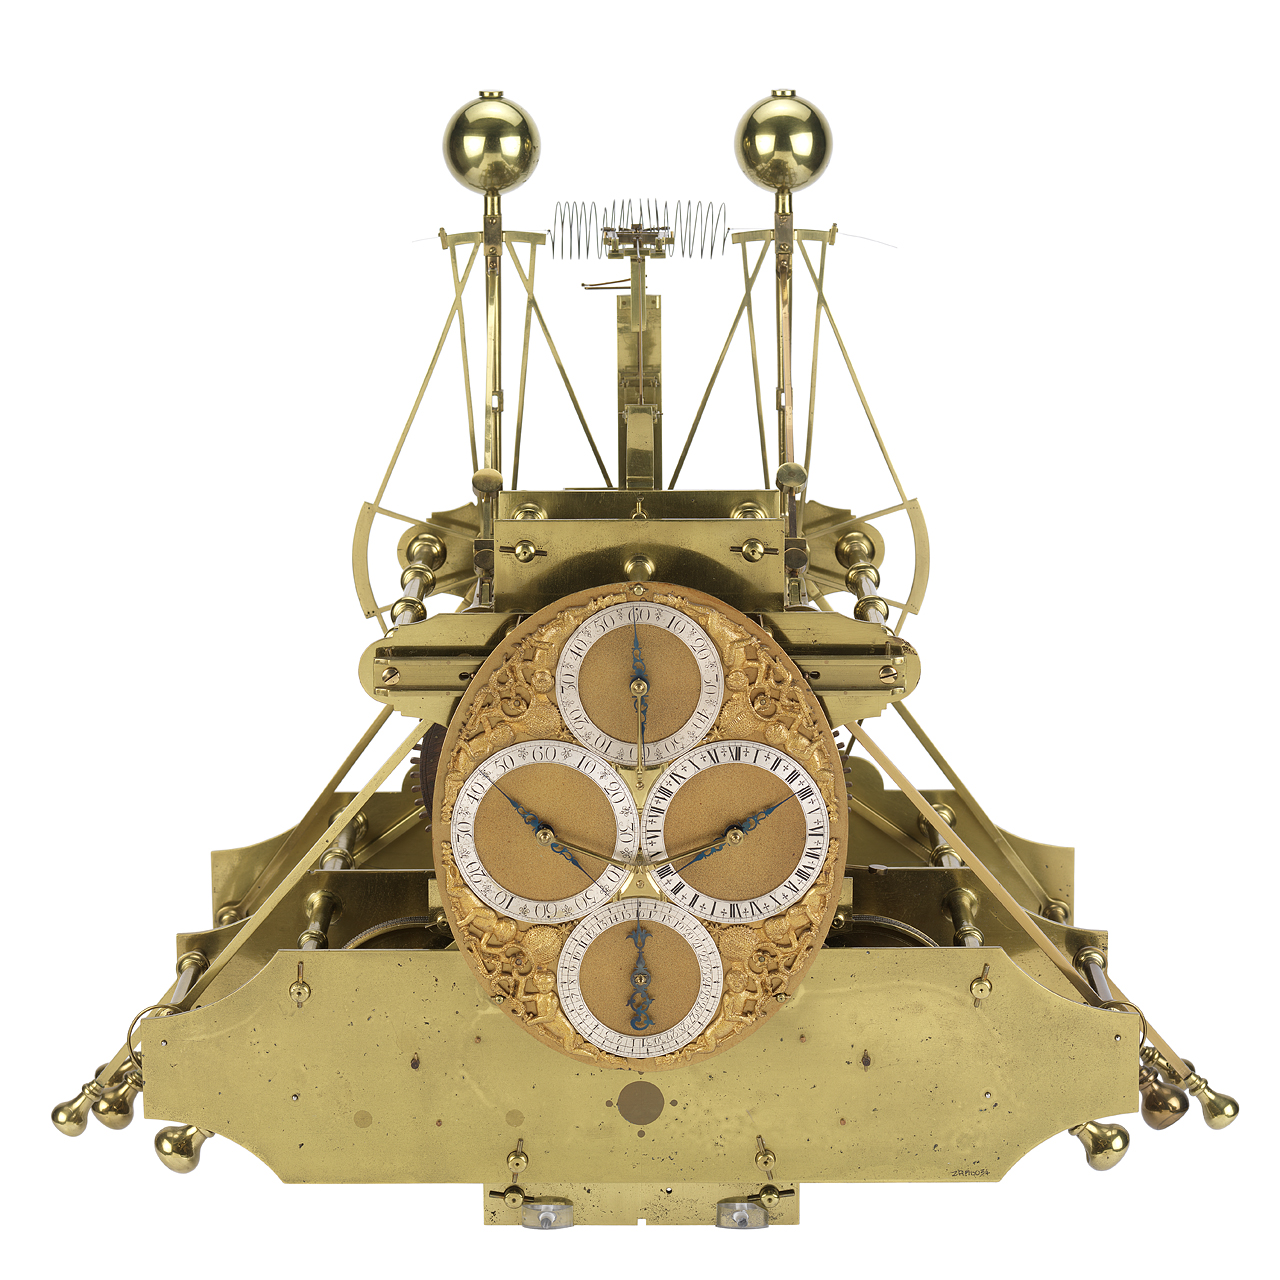
\includegraphics[width=0.2\textwidth]{kugel/H1.jpg}} 
\quad \quad
\centering
    \subfigure[H2 - 1737]{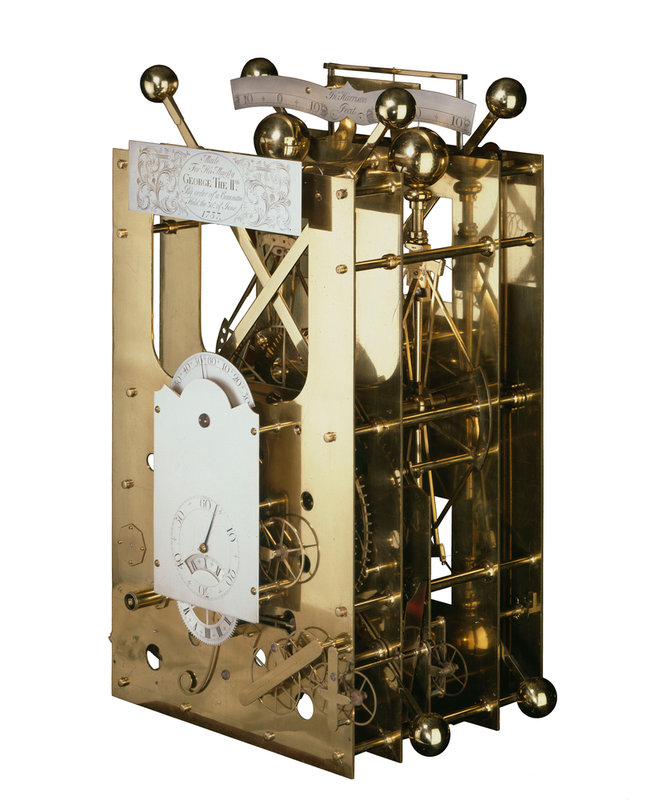
\includegraphics[width=0.2\textwidth]{kugel/H2.jpg}} 
\quad \quad
\centering
    \subfigure[H4 - 1753]{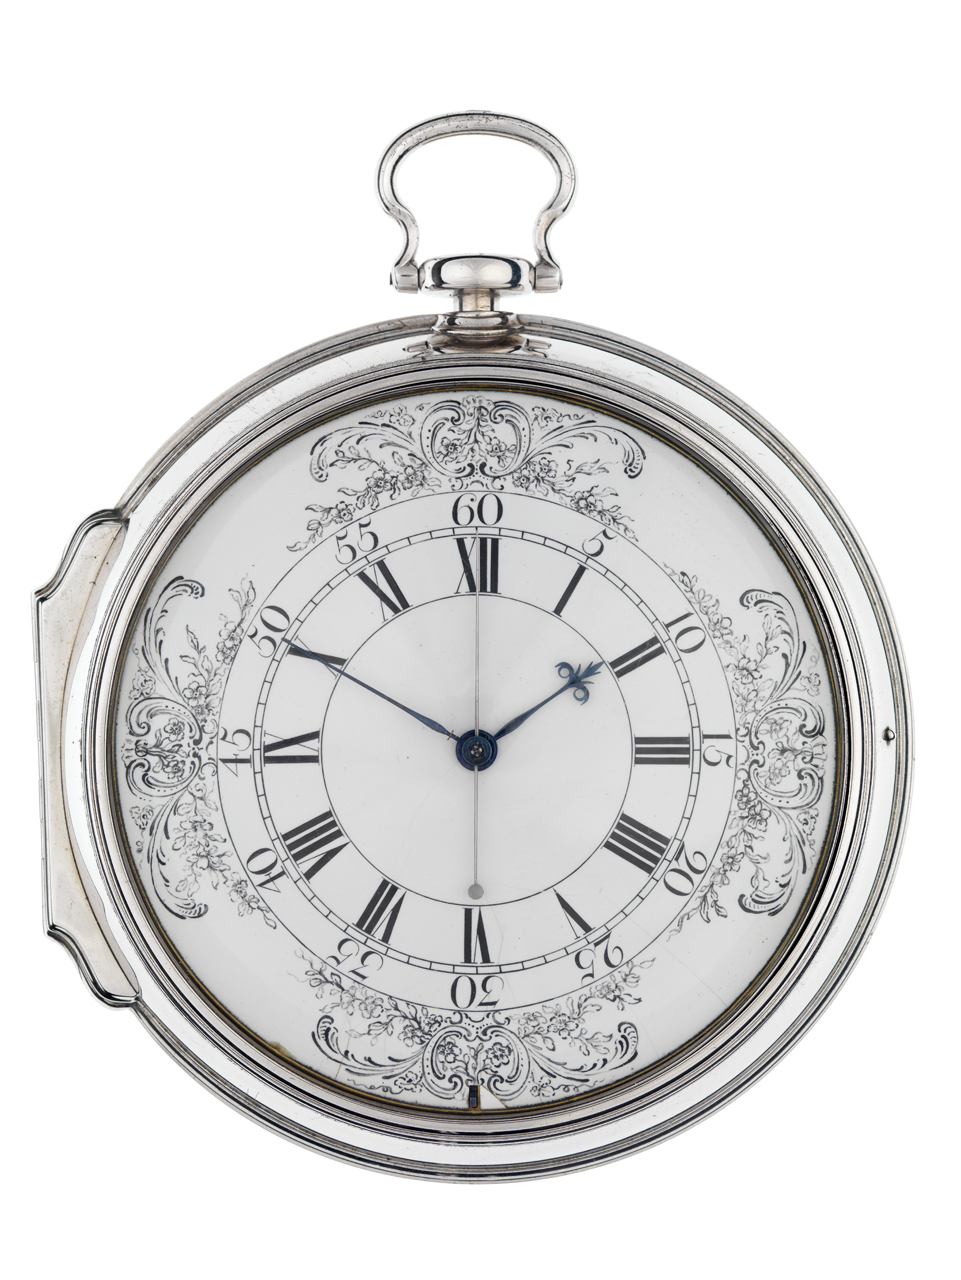
\includegraphics[width=0.2\textwidth]{kugel/H4.jpg}} 
\quad \quad
\centering
    \subfigure[H4 - 1753]{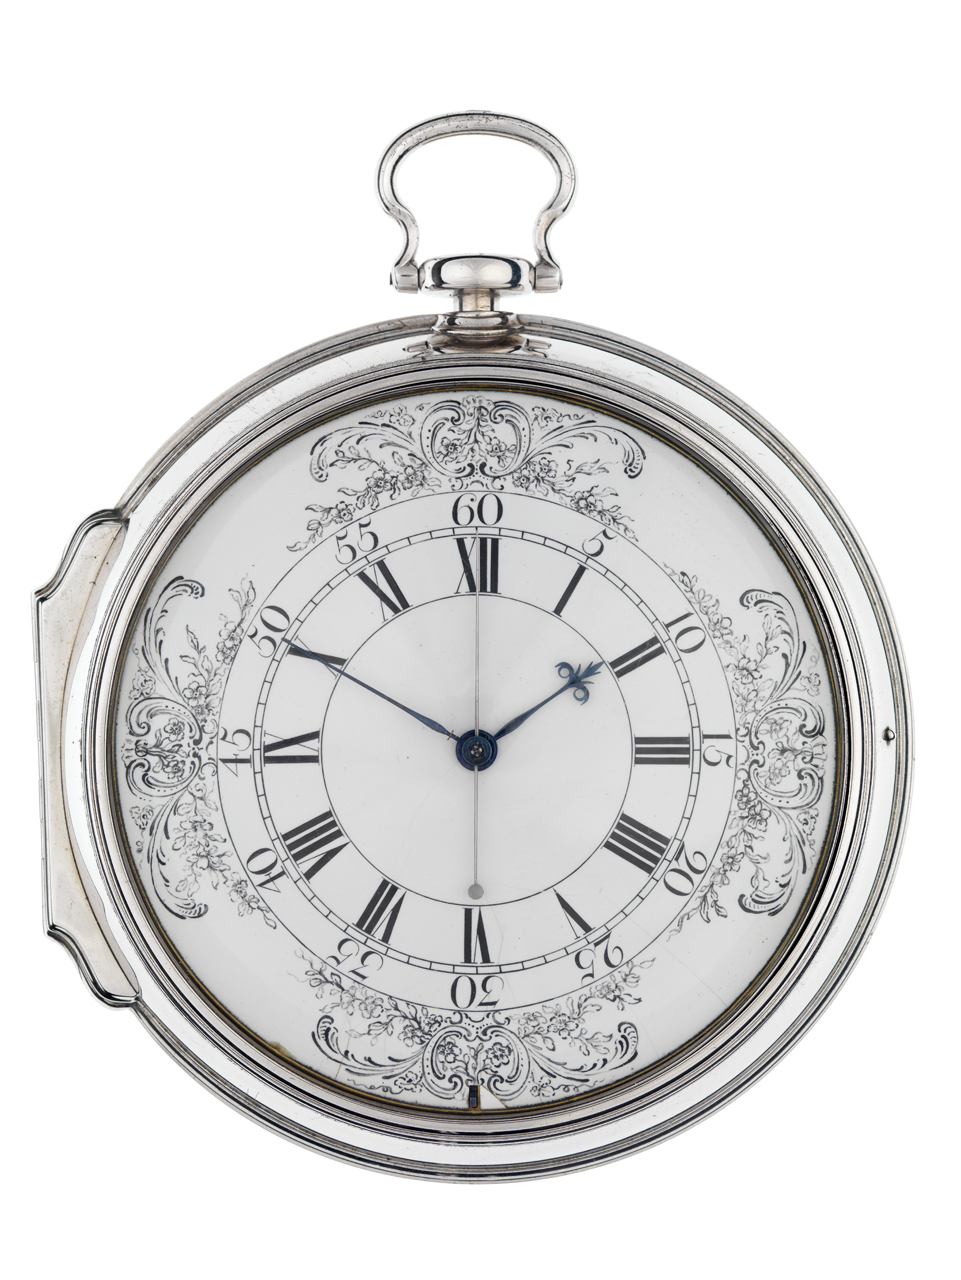
\includegraphics[width=0.2\textwidth]{kugel/H4.jpg}} 
\caption{Sphärisches Dreieck an der Himmelskugel mit den zu ermittelnden Längen} 
\end{figure}


\subsection{Bestimmung des Längengrades} \label{BestimmungL} 
Zur Bestimmung des Längengrades verwenden wir den Seitenkosinussatz:
\begin{align*}
\cos(c) = \cos(a)\cos(b) + \sin(a)\sin(b)\cos(\gamma)
\end{align*}

Auf unsere Seiten angewendet können wir einsetzen

\begin{align*}
\cos(\overline{ZS}) &= \cos(\overline{NZ}) \cos(\overline{NS}) + \sin(\overline{NZ}) \sin(\overline{NS}) \cos(\tau) \\
\Rightarrow \quad \quad
\cos(90^{\circ} - h) &= \cos(90^{\circ} - \phi) \cos(90^{\circ} - \delta) + \sin(90^{\circ} - \phi)\sin(90^{\circ} - \delta) \cos(\tau)
\end{align*}

Nach dem uns unbekannten Winkel $\tau$ aufgelöst ergibt die Gleichung
\begin{align*}
\tau &= \arccos 
\frac{ \cos(90^{\circ} - \phi) \cos(90^{\circ} - \delta) - \cos(90^{\circ} - h)} {\sin(90^{\circ} - \phi)\sin(90^{\circ} - \delta)}
\end{align*}

Der Winkel $\tau$ setzt sich aus folgenden Komponenten zusammen
\begin{align*}
\cos (\tau) &= \cos (t - e_\delta - \lambda) 
\end{align*}

Die zugehörigen bekannten Grössen sind:
\begin{itemize}
\item Zeit ($t$) $\Rightarrow$ Uhr
\item Rektazension ($e_\delta$) $\Rightarrow$ Sternatlas, Almanach, App 
\item Längengrad ($\lambda$) $\Rightarrow$ Der Längengrad unseres Standorts ist die einzige Unbekannte
\end{itemize}


\subsection{Sternzeit}
Für die Positionsbestimmung auf der Erde ist die Sonne nicht der beste Stern, welchen man auswählen kann. Sie ist nur am Tag zu sehen und man kann nur eine Messung durchführen, was zu einem relativ ungenauen Ergebnis führt. Zudem kann man die Messergebnisse nur verwenden, wenn die Sonne zu diesem Zeitpunkt im Zenit stand. Ansonsten ist das Messergebnis unbrauchbar. Aufgrund ihrer Grösse am Himmel ist es auch schwierig einen Punkt anzupeilen. Hinzukommt die Helligkeit der Sonne. Würde man sie direkt ansehen, führt das eher zu Blindheit als zu einem Messergebnis.
Nichts desto trotz haben die Menschen schon je her Aufzeichnungen über die verschiedenen Sonnenstände an der Himmelskugel gemacht. Auch heute noch werden Nautische Karten verwendet, um den genauen Sonnenstand zu ermitteln oder die Abweichung zu erhalten, welche von der nicht exakten elliptischen Erdumlaufbahn entsteht.

Sterne eignen sich zur Bestimmung der Position dafür umso besser. Sie befinden sich immer am selben Ort und bewegen sich nicht. Zudem kann man mehrere Sterne messen, was zu einem genaueren Ergebnis führt. Da die Erdumdrehung nicht exakt 24 Stunden dauert, wird zwischen Sonnen- und Sternzeit unterschieden.

\begin{center}
\begin{tabular}{cc}
Sonnenzeit & 24:00:00 Stunden \\
Sternzeit & 23:56:04 Stunden
\end{tabular}
\end{center}

Der Sterntag geht somit etwa 4 Minuten kürzer als der Sonnentag. Dies lässt sich damit begründen, dass sich die Sonne ein wenig langsamer als die Sterne um die Erde bewegt. Dies lässt sich auf die Bewegung der Erde um die Sonne abstützen.

Wenn man nun Sterne zur Positionsbestimmung verwenden möchte, muss man die Sternzeit zuerst in die Sonnenzeit umrechnen, um auf das richtige Ergebnis zu kommen. Auf dieses Thema gehen wir in dieser Arbeit aber nicht genauer ein.


\subsection{Breitengrad bekannt? - Breite nicht bekannt!}

In den vorherigen Berechnungen sind wir immer davon ausgegangen, dass uns die Breite bekannt ist. Dies ist in Wirklichkeit aber nicht so, denn auf dem offenen Meer hat man keinerlei Anhaltspunkte, wo man sein könnte.

Im Kapitel~\ref{BreitengradM} \nameref{BreitengradM} haben wir aber gesehen, dass sich dieser relativ einfach und ohne grossen Aufwand bestimmen lässt. Damit wir auf See eine verlässliche Messung erhalten, benötigen wir mindestens zwei Sterne. Mit diesen beiden Messungen kann man den Messfehler minimieren und den Standort relativ genau bestimmen.

Da wir zwei Sterne haben, benötigen wir auch zwei Gleichungen mit zwei Unbekannten
\begin{align*}
\cos(\overline{ZS_1}) &= \cos(\overline{NZ}) \cos(\overline{NS_1}) + \sin(\overline{NZ}) \sin(\overline{NS_1}) \cos(\tau_1) \\
\cos(\overline{ZS_2}) &= \cos(\overline{NZ}) \cos(\overline{NS_2}) + \sin(\overline{NZ}) \sin(\overline{NS_2}) \cos(\tau_2) \\
\\
\Rightarrow \quad \quad
\cos(90^{\circ} - h_1) &= \cos(90^{\circ} - \phi) \cos(90^{\circ} - \delta_1) + \sin(90^{\circ} - \phi)\sin(90^{\circ} - \delta_1) \cos(\tau_1) \\
\Rightarrow \quad \quad
\cos(90^{\circ} - h_2) &= \cos(90^{\circ} - \phi) \cos(90^{\circ} - \delta_2) + \sin(90^{\circ} - \phi)\sin(90^{\circ} - \delta_2) \cos(\tau_2)
\end{align*}

Diese Gleichungen lassen sich nur mit Hilfe eines Computers oder viel Geduld und Zeit lösen. Die Hilfe des Computers ist heutzutage kein Problem, jedoch gab es diesen zur Zeit der Entdecker und Seefahrer nicht. Da kommt die Geduld und die Zeit ins Spiel, denn diese war auf einem Schiff auf offener See reichlich vorhanden.


\section{Übungsaufgabe}
Um es den alten Seefahrern gleichzutun und seinen eigenen Standort herauszufinden, können Sie in der folgenden Übungsaufgabe in ihre Fussstapfen treten und die alten Berechnungsmethoden anwenden.

Folgende Messwerte stellen wir Ihnen zur Verfügung und wurden bereits gemessen oder abgelesen.
Mit Hilfe des Sextanten, konnten folgende Werte ermittelt werden.

\begin{center}
\renewcommand{\arraystretch}{1.5}
\begin{tabular}{cc}
Elevation der Sonne $h$ & $26^{\circ}$ 18’ 00.000’’\\
Geografische Breite ($\phi$) & $47^{\circ}$ 13’ 24.751’’ N
\end{tabular}
\end{center}

Durch die Aufzeichnungen im nautischen Jahrbuch, wissen wir folgende Angaben:

\begin{center}
\renewcommand{\arraystretch}{1.5}
\begin{tabular}{cccc}
Deklination der Sonne ($\delta$) & $17^{\circ}$ 16’ 01.200’’ \\
Rektaszension der Sonne ($e_\delta$) & $03^{\circ}$ 03’ 14.400’’ \\
Kulmination der Sonne & 13h 21min 18s \\
Merediandurchgang der Sonne & 11h 56min 29s
\end{tabular}
\end{center}

Die Zeitdifferenz zur \textit{Coordinated Universal Time (UTC)} beträgt eine Stunde. Im Sommer müssen wir aber wegen der in der Zeitzone \textit{Greenwich Mean Time (GMT)} verwendeten Sommerzeit noch eine Stunde dazurechnen. Somit ergeben sich im Sommer zwei Stunden Zeitunterschied.\\ 


Das Ziel der Berechnung ist, den fehlenden Längengrad zu berechnen. Nur mit diesem in Kombination mit dem Breitengrad, ist es uns möglich den genauen Standort herauszufinden. \\

\textit{Lösung:} \\
Der Lösungsansatz, verbirgt sich hinter dem nach dem Stundenwinkel $\tau$ umgeformten Seitenkosinussatz

\begin{align*}
\tau = \arccos 
\frac{ \cos(90^{\circ} - \phi) \cos(90^{\circ} - \delta) - \cos(90^{\circ} - h)} {\sin(90^{\circ} - \phi)\sin(90^{\circ} - \delta)}
\end{align*}
Die gesuchten Werte können wir mithilfe der Informationen des Sextanten und des nautischen Jahrbuchs berechnen.
\begin{align*}
90^{\circ} - \phi &= 42.778^{\circ}
\\
90^{\circ} - \delta &= 72.733^{\circ}
\\
90^{\circ} - h &= 63.700^{\circ}
\end{align*}
Eingesetzt in den nach $\tau$ umgeformten Seitenkosinussatz, erhalten wir für $\tau$ folgendes Ergebnis
\begin{align*}
\tau = 110.319^{\circ} 
\end{align*}
Durch den direkten Zusammenhang der Koordinaten zwischen Bogenmass und Stunden, lässt sich das Bogenmass in Stunden umrechnen
\begin{align*}
\tau = 7.3546h
\end{align*}
Um den gesuchten Längengrad nun zu erhalten, müssen wir $\tau$ in ihre Komponenten Zeit (t), Rektaszension der Sonne ($e_\delta$) und unseren gesuchten Längengrad ($\lambda$ zerlegen
\begin{align*}
\tau &= t - e_\delta - \lambda 
\end{align*}


Für die Berechnung von t kommt die Uhr von Harrison ins Spiel. Wir wissen, dass die Sonne in unserem Heimathafen London am Mittag kulminiert. Das heisst um 12.00 Uhr steht sie im Zenit und ist somit senkrecht über uns. 
Befinden wir uns nicht am selben Standort, kulminiert die Sonne nicht genau um 12.00 Uhr sondern früher oder später.
In unserem Fall, findet diese 13.355h nach Mitternacht statt. Für diese Zeitangabe benötigten die Seefahrer die Uhr, um eine exakte Zeitangabe zu treffen. Kleine Abweichungen in der Zeitmessung, hätten Kilometerweite Abweichungen in der Standortbestimmung zur Folge.
Um die Zeitdifferenz nun zu berechnen, müssen wir unsere Kulmination mit dieser unseres Heimathafens in London subtrahieren 
\begin{align*}
13.355h - 12.000h &= 1.3555h
\end{align*}

Um die Differenz der Zeit und somit die Zeitzonen der Erde noch miteinzubeziehen, müssen den Zeitunterschied zwischen den beiden Zeitzonen GMT und UTC miteinbeziehen. Achtung: Es ist Sommer, also sind es zwei Stunden Unterschied.
\begin{align*}
1.3555h - 2.000h &= -0.645h
\end{align*}

Die Rektaszension der Sonne $e_\delta$ lässt sich aus dem Sternatlas herauslesen und ist in Stunden
\begin{align*}
03^{\circ} 03 14.400 &= 0.2036h
\end{align*}

Der Merediandurchgang eines Tages ist nicht immer gleich, sprich nicht jeder Sonnentag ist gleich lang. Dies muss berücksichtigt werden, da sich die Abweichung direkt auf die Genauigkeit des Längengrades niederschlägt.
Die Zeitdifferenz berechnet sich aus dem vollen Sonnentag von 12h und dem aktuellen Merediandurchgang
\begin{align*}
\text{12:00:00 - 11:56:29 = 0:03:31 = 0.0586h}
\end{align*}




XXXX




Dieser Betrag dazu addiert ergibt
\begin{align*}
-0.645 h + 0.0586 h = - 0.5863 h = \lambda
\end{align*}

Umgerechnet in Bogenmass ergibt sich für $\lambda$
\begin{align*}
\lambda = - 8.7945^{\circ} = -8^{\circ} 47 40.2 
\end{align*}



Daraus ergeben sich folgende Koordinaten, mit welchen wir unseren genauen Standort ermitteln können
\begin{align*}
8^{\circ}47 40.2 E \\
47^{\circ}13 24.751 N
\end{align*}




\printbibliography[heading=subbibliography]
\end{refsection}







